%
%
\documentclass[a4paper,pagesize=dvips,onecolumn,11pt,titlepage,twoside]{scrartcl}
% \documentclass[a4paper,dvips,onecolumn,11pt,titlepage]{scrreprt}
\usepackage{qgis_style}

\begin{document}

%  !TeX  root  =  user_guide.tex

\begin{titlepage}
%\addcontentsline{toc}{section}{Titre}
\begin{center}

%\begin{figure}[H]
\begin{center}

\includegraphics{qgislogo} 
\end{center}
%\end{figure}

\Huge{Quantum GIS}\\
\vspace{0.5cm}
\Large{User Guide} \\
\vspace{0.5cm}
%
\includegraphics[clip=true, scale=0.4]{splash} 
\Large{Version ~\CURRENT \textsl{'This is no moon !'}}

\end{center}
\end{titlepage}

%  !TeX  root  =  user_guide.tex
\frontmatter
\pagestyle{scrplain}
\addchap{Préambule}
\vspace{1cm}
Ce document est le manuel officiel d'utilisation du logiciel \QG. Les logiciels et le matériel décrits dans ce document sont pour la plupart des marques déposées et donc soumises à des obligations légales. \QG est distribué sous la Licence publique générale GNU (GPL). Vous trouverez plus d'informations sur la page internet de \QG \url{http://qgis.osgeo.org}.
\par\bigskip
Les détails, données, résultats, etc. inclus dans ce document ont été écrits et vérifiés au mieux des connaissances des auteurs et des éditeurs. Néanmoins, des erreurs dans le contenu sont possibles.
\par\bigskip
Ainsi l'ensemble des données ne saurait faire l'objet d'une garantie. Les auteurs et les éditeurs ne sauraient être responsables de tout dommage direct, indirect, secondaire ou accessoire découlant de l'utilisation de ce manuel. Les éventuelles corrections sont toujours les bienvenues.
\par\bigskip
Ce document a été rédigé avec \LaTeX. Les sources sont disponibles en code \LaTeX{} via\\ \url{https://svn.osgeo.org/qgis/docs/tags/1.3.0_user_guide} et en PDF via \url{http://qgis.osgeo.org/documentation/manuals.html}. 
Des versions traduites peuvent être téléchargées via la section de documentation du projet QGIS. Pour plus d'informations sur les manières de contribuer à ce document et à sa traduction, veuillez visiter \url{http://www.qgis.org/wiki/} 

\vspace{1cm}
\noindent
\textbf{Références de ce document}
\par\bigskip
Ce document contient des références internes et externes sous forme de lien. Cliquer sur un lien interne provoque un déplacement dans le document, tandis que cliquer sur un lien externe ouvrira une adresse internet dans le navigateur par défaut. En PDF, les liens internes seront indiqués en bleu et les externes en rouge. En HTML, le navigateur affiche et gère les deux types de liens de la même fa\c{c}on.

\newpage

\begin{flushleft}
\textbf{Auteurs et éditeurs :}
 \par\bigskip\noindent
\begin{tabular}{p{4cm} p{4cm} p{4cm}}
Tara Athan & Radim Blazek & Godofredo Contreras   \\
 Otto Dassau & Martin Dobias & Claudia A. Engel \\ 
 Carson J.Q. Farmer &J\"urgen E. Fischer & Anne Ghisla \\
Stephan Holl &  Magnus Homann& Marco Hugentobler \\ 
 Lars Luthman & Gavin Macaulay & Werner Macho \\
  Tyler Mitchell & Brendan Morely&Gary E. Sherman\\
  Tim Sutton & David Willis \\ \
\end{tabular}
\end{flushleft}

\begin{flushleft}
\textbf{Traducteurs version francophone:}
  \par\bigskip\noindent
\begin{tabular}{p{4cm} p{4cm} p{4cm}}
Benjamin Bohard & Jeremy Garniaux & Yves Jacolin \\
Stéphane Morel & Jean Roc Morreale & Marie Silvestre \\
Tahir Tamba & Xavier M. & Cyril de Runz \\
Benjamin Lerre \\
\end{tabular}
\end{flushleft}

Nos remerciements vont à Bertrand Masson pour son aide précieuse quant à la mise en page de ce document, Tisham Dhar pour avoir préparé l'environnement initial de documentation pour MS Windows, à Tom Elwertowski et William Kyngesburye pour la section d'installation sur Mac OS X et à Carlos  D\'{a}vila, Paolo Cavallini et Christian Gunning pour les révisions. Si nous avons négligé de citer ici le nom d'un contributeur, veuillez accepter nos excuses pour cet oubli et nous le signaler pour correction.
\par\bigskip\noindent
\textbf{Copyright \copyright~2004 - 2010 \QG Development Team}
\par\bigskip\noindent
\textbf{Internet :} \url{http://qgis.osgeo.org}

\addsec{Licence de ce document}

La permission de copier, distribuer, modifier ce document est accordée sous les termes de la GNU Free Documentation License, dans sa version 1.3 ou plus récente telle que publiée par la Free Software Foundation; sans modification de son contenu, sans ajouts la précédant ou la suivant. Une copie peut être lue dans la section \ref{label_fdl} nommée "GNU Free Documentation License".

\newpage


\renewcommand{\baselinestretch}{1.0}
\parskip0.7ex

\addcontentsline{toc}{section}{Inhaltsverzeichnis}
\tableofcontents
\newpage

\addcontentsline{toc}{section}{Abbildungsverzeichnis}
\listoffigures
\newpage

\addcontentsline{toc}{section}{Tabellenverzeichnis}
\listoftables
\newpage

\addcontentsline{toc}{section}{Verzeichnis der QGIS Hinweise}
\listof{Tip}{QGIS Hinweise}
\newpage

\renewcommand{\baselinestretch}{1.1} 
\parskip1.5ex

%% vim:textwidth=76:autoindent

\section{Introduction}\label{label_introduction}
\pagenumbering{arabic}
\setcounter{page}{1}

The majority of this document is devoted to describing how to build
QGIS~\CURRENT
(\textit{`TITAN'}) from the source distribution. These instructions are for
Linux/Unix and other POSIX systems which have the required build
environment. If you are building on FreeBSD, see
\url{http://qgis.org/index.php?option=com_content&task=view&id=84&Itemid=86} for hints and further
information.

Installing on Windows and Mac OS X is a simple process as described
below.

You don't have to build all the QGIS dependencies from source. If your
platform provides packages at an acceptable version for the needed
dependencies, you can install them prior to building QGIS. Make sure you
also install the "development" package (if separate from the main package)
for each dependency. QGIS needs the header files from these packages in
order to build. 

The latest version of this document can always be found at 
\url{http://qgis.org/index.php?option=com_content&task=view&id=106&Itemid=89}.

% vim: set textwidth=78 autoindent:

\section{Writing a QGIS Plugin in C++}\label{cpp_plugin}

% when the revision of a section has been finalized, 
% comment out the following line:
\updatedisclaimer

In this section we provide a beginner's tutorial for writing a simple QGIS
C++ plugin. It is based on a workshop held by Dr. Marco Hugentobler. 

QGIS C++ plugins are dynamically linked libraries (.so or .dll). They are
linked to QGIS at runtime when requested in the plugin manager and extend the
functionality of QGIS. They have access to the QGIS GUI and can be devided
into core and external plugins.

Technically the QGIS plugin manager looks in the lib/qgis directory for all
.so files and loads them when it is started. When it is closed they are
unloaded again, except the ones with a checked box. For newly loaded plugins,
the \method{classFactory} method creates an instance of the plugin class and
the \method{initGui} method of the plugin is called to show the GUI elements
in the plugin menu and toolbar. The \method{unload()} function of the plugin
is used to remove the allocated GUI elements and the plugin class itself is
removed using the class destructor. To list the plugins, each plugin must
have a few external 'C' functions for description and of course the
\method{classFactory} method.

\subsection{Why C++ and what about licensing}

QGIS itself is written in C++, so it also makes sense to write plugins in C++
as well. It is an object-oriented programming (OOP) language that is viewed
by many developers as a prefered language for creating large-scale
applications.

QGIS C++ plugins use functionalities of libqgis*.so libraries. As they are
licensed under GNU GPL, QGIS C++ plugins must be licenced under the GPL, too.
This means you may use your plugins for any purpose and you are not forced to
publish them. If you do publish them however, they must be published under
the conditions of the GPL license. 

\subsection{Programming a QGIS C++ Plugin in four steps}

The example plugin is a point converter plugin and intentionally kept simple. 
The plugin searches the active vector layer in QGIS, converts all vertices of
the layer features to point features keeping the attributes and finally
writes the point features into a delimited text file. The new layer can then
be loaded into QGIS using the delimited text plugin (see Section
\ref{label_dltext}).

\minisec{Step 1: Make the plugin manager recognise the plugin}

As a first step we create the \filename{QgsPointConverter.h} and
\filename{QgsPointConverter.cpp} files. Then we add virtual methods inherited
from QgisPlugin (but leave them empty for now), create necessary external 'C'
methods and a .pro file, which is a Qt mechanism to easily create Makefiles.
Then we compile the sources, move the compiled library into the plugin folder
and load it in the QGIS plugin manager.

\textbf{a) Create new pointconverter.pro file and add}:

\begin{verbatim}
#base directory of the qgis installation
QGIS_DIR = /home/marco/src/qgis

TEMPLATE = lib
CONFIG = qt
QT += xml qt3support
unix:LIBS += -L/$$QGIS_DIR/lib -lqgis_core -lqgis_gui
INCLUDEPATH += $$QGIS_DIR/src/ui $$QGIS_DIR/src/plugins  $$QGIS_DIR/src/gui \
	       $$QGIS_DIR/src/raster $$QGIS_DIR/src/core $$QGIS_DIR 
SOURCES = qgspointconverterplugin.cpp
HEADERS = qgspointconverterplugin.h
DEST = pointconverterplugin.so
DEFINES += GUI_EXPORT= CORE_EXPORT=
\end{verbatim}

\textbf{b) Create new qgspointconverterplugin.h file and add}:

\begin{verbatim}
#ifndef QGSPOINTCONVERTERPLUGIN_H
#define QGSPOINTCONVERTERPLUGIN_H

#include "qgisplugin.h"

/**A plugin that converts vector layers to delimited text point files.
 The vertices of polygon/line type layers are converted to point features*/
class QgsPointConverterPlugin: public QgisPlugin
{
  public:
  QgsPointConverterPlugin(QgisInterface* iface);
  ~QgsPointConverterPlugin();
  void initGui();
  void unload();
  
  private:
  QgisInterface* mIface;
};
#endif
\end{verbatim}

\textbf{c) Create new qgspointconverterplugin.cpp file and add}:

\begin{verbatim}
#include "qgspointconverterplugin.h"

#ifdef WIN32
#define QGISEXTERN extern "C" __declspec( dllexport )
#else
#define QGISEXTERN extern "C"
#endif

QgsPointConverterPlugin::QgsPointConverterPlugin(QgisInterface* iface): mIface(iface)
{
}

QgsPointConverterPlugin::~QgsPointConverterPlugin()
{
}

void QgsPointConverterPlugin::initGui()
{
}

void QgsPointConverterPlugin::unload()
{
}

QGISEXTERN QgisPlugin* classFactory(QgisInterface* iface)
{
  return new QgsPointConverterPlugin(iface);
}

QGISEXTERN QString name()
{
  return "point converter plugin";
}

QGISEXTERN QString description()
{
  return "A plugin that converts vector layers to delimited text point files";
}

QGISEXTERN QString version()
{
  return "0.00001";
}

// Return the type (either UI or MapLayer plugin)
QGISEXTERN int type()
{
  return QgisPlugin::UI;
}

// Delete ourself
QGISEXTERN void unload(QgisPlugin* theQgsPointConverterPluginPointer)
{
  delete theQgsPointConverterPluginPointer;
}
\end{verbatim}

\minisec{Step 2: Create an icon, a button and a menu for the plugin}

This step includes adding a pointer to the QgisInterface object in the plugin
class. Then we create a QAction and a callback function (slot), add it to the
QGIS GUI using QgisIface::addToolBarIcon() and QgisIface::addPluginToMenu()
and finally remove the QAction in the \method{unload()} method.

\textbf{d) Open qgspointconverterplugin.h again and extend existing content to}:

\begin{verbatim}
#ifndef QGSPOINTCONVERTERPLUGIN_H
#define QGSPOINTCONVERTERPLUGIN_H

#include "qgisplugin.h"
#include <QObject>

class QAction;

/**A plugin that converts vector layers to delimited text point files.
 The vertices of polygon/line type layers are converted to point features*/
class QgsPointConverterPlugin: public QObject, public QgisPlugin
{
  Q_OBJECT

 public:
  QgsPointConverterPlugin(QgisInterface* iface);
  ~QgsPointConverterPlugin();
  void initGui();
  void unload();
  
 private:
  QgisInterface* mIface;
  QAction* mAction;
  
   private slots:
   void convertToPoint();
};

#endif
\end{verbatim}

\textbf{e) Open qgspointconverterplugin.cpp again and extend existing content to}:

\begin{verbatim}
#include "qgspointconverterplugin.h"
#include "qgisinterface.h"
#include <QAction>

#ifdef WIN32
#define QGISEXTERN extern "C" __declspec( dllexport )
#else
#define QGISEXTERN extern "C"
#endif

QgsPointConverterPlugin::QgsPointConverterPlugin(QgisInterface* iface): \
    mIface(iface), mAction(0)
{

}

QgsPointConverterPlugin::~QgsPointConverterPlugin()
{

}

void QgsPointConverterPlugin::initGui()
{
  mAction = new QAction(tr("&Convert to point"), this);
  connect(mAction, SIGNAL(activated()), this, SLOT(convertToPoint()));
  mIface->addToolBarIcon(mAction);
  mIface->addPluginToMenu(tr("&Convert to point"), mAction);
}

void QgsPointConverterPlugin::unload()
{
  mIface->removeToolBarIcon(mAction);
  mIface->removePluginMenu(tr("&Convert to point"), mAction);
  delete mAction;
}

void QgsPointConverterPlugin::convertToPoint()
{
  qWarning("in method convertToPoint");
}

QGISEXTERN QgisPlugin* classFactory(QgisInterface* iface)
{
  return new QgsPointConverterPlugin(iface);
}

QGISEXTERN QString name()
{
  return "point converter plugin";
}

QGISEXTERN QString description()
{
  return "A plugin that converts vector layers to delimited text point files";
}

QGISEXTERN QString version()
{
  return "0.00001";
}

// Return the type (either UI or MapLayer plugin)
QGISEXTERN int type()
{
  return QgisPlugin::UI;
}

// Delete ourself
QGISEXTERN void unload(QgisPlugin* theQgsPointConverterPluginPointer)
{
  delete theQgsPointConverterPluginPointer;
}
\end{verbatim}


\minisec{Step 3: Read point features from the active layer and write to text file}

To read the point features from the active layer we need to query the current
layer and the location for the new text file. Then we iterate through all
features of the current layer, convert the geometries (vertices) to points,
open a new file and use QTextStream to write the x- and y-coordinates
into it.

\textbf{f) Open qgspointconverterplugin.h again and extend existing content to}

\begin{verbatim}
class QgsGeometry;
class QTextStream;

private:

void convertPoint(QgsGeometry* geom, const QString& attributeString, \
		  QTextStream& stream) const;
void convertMultiPoint(QgsGeometry* geom, const QString& attributeString, \
		  QTextStream& stream) const;
void convertLineString(QgsGeometry* geom, const QString& attributeString, \
		  QTextStream& stream) const;
void convertMultiLineString(QgsGeometry* geom, const QString& attributeString, \
		  QTextStream& stream) const;
void convertPolygon(QgsGeometry* geom, const QString& attributeString, \
		  QTextStream& stream) const;
void convertMultiPolygon(QgsGeometry* geom, const QString& attributeString, \
		  QTextStream& stream) const;
\end{verbatim}

\textbf{g) Open qgspointconverterplugin.cpp again and extend existing content to}:

\begin{verbatim}
#include "qgsgeometry.h"
#include "qgsvectordataprovider.h"
#include "qgsvectorlayer.h"
#include <QFileDialog>
#include <QMessageBox>
#include <QTextStream>

void QgsPointConverterPlugin::convertToPoint()
{
  qWarning("in method convertToPoint");
  QgsMapLayer* theMapLayer = mIface->activeLayer();
  if(!theMapLayer)
    {
      QMessageBox::information(0, tr("no active layer"), \
      tr("this plugin needs an active point vector layer to make conversions \ 
          to points"), QMessageBox::Ok);
      return;
    }
  QgsVectorLayer* theVectorLayer = dynamic_cast<QgsVectorLayer*>(theMapLayer);
  if(!theVectorLayer)
    {
      QMessageBox::information(0, tr("no vector layer"), \
      tr("this plugin needs an active point vector layer to make conversions \
          to points"), QMessageBox::Ok);
      return;
    }
  
  QString fileName = QFileDialog::getSaveFileName();
  if(!fileName.isNull())
    {
      qWarning("The selected filename is: " + fileName);
      QFile f(fileName);
      if(!f.open(QIODevice::WriteOnly))
      {
	QMessageBox::information(0, "error", "Could not open file", QMessageBox::Ok);
	return;
      }
      QTextStream theTextStream(&f);
      theTextStream.setRealNumberNotation(QTextStream::FixedNotation);

      QgsFeature currentFeature;
      QgsGeometry* currentGeometry = 0;

      QgsVectorDataProvider* provider = theVectorLayer->dataProvider();
      if(!provider)
      {
          return;
      }

      theVectorLayer->select(provider->attributeIndexes(), \
      theVectorLayer->extent(), true, false);

      //write header
      theTextStream << "x,y";
      theTextStream << endl;

      while(theVectorLayer->nextFeature(currentFeature))
      {
	 QString featureAttributesString;
      
        currentGeometry = currentFeature.geometry();
        if(!currentGeometry)
        {
            continue;
        }

        switch(currentGeometry->wkbType())
        {
            case QGis::WKBPoint:
            case QGis::WKBPoint25D:
                convertPoint(currentGeometry, featureAttributesString, \
		theTextStream);
                break;

            case QGis::WKBMultiPoint:
            case QGis::WKBMultiPoint25D:
                convertMultiPoint(currentGeometry, featureAttributesString, \
		theTextStream);
                break;

            case QGis::WKBLineString:
            case QGis::WKBLineString25D:
                convertLineString(currentGeometry, featureAttributesString, \
		theTextStream);
                break;

            case QGis::WKBMultiLineString:
            case QGis::WKBMultiLineString25D:
                convertMultiLineString(currentGeometry, featureAttributesString \
		theTextStream);
                break;

            case QGis::WKBPolygon:
            case QGis::WKBPolygon25D:
                convertPolygon(currentGeometry, featureAttributesString, \
		theTextStream);
                break;

            case QGis::WKBMultiPolygon:
            case QGis::WKBMultiPolygon25D:
                convertMultiPolygon(currentGeometry, featureAttributesString, \
		theTextStream);
                break;
        }
      }
    }
}

//geometry converter functions
void QgsPointConverterPlugin::convertPoint(QgsGeometry* geom, const QString& \
attributeString, QTextStream& stream) const
{
    QgsPoint p = geom->asPoint();
    stream << p.x() << "," << p.y();
    stream << endl;
}

void QgsPointConverterPlugin::convertMultiPoint(QgsGeometry* geom, const QString& \
attributeString, QTextStream& stream) const
{
    QgsMultiPoint mp = geom->asMultiPoint();
    QgsMultiPoint::const_iterator it = mp.constBegin();
    for(; it != mp.constEnd(); ++it)
    {
        stream << (*it).x() << "," << (*it).y();
        stream << endl;
    }
}

void QgsPointConverterPlugin::convertLineString(QgsGeometry* geom, const QString& \
attributeString, QTextStream& stream) const
{
    QgsPolyline line = geom->asPolyline();
    QgsPolyline::const_iterator it = line.constBegin();
    for(; it != line.constEnd(); ++it)
    {
        stream << (*it).x() << "," << (*it).y();
        stream << endl;
    }
}

void QgsPointConverterPlugin::convertMultiLineString(QgsGeometry* geom, const QString& \
attributeString, QTextStream& stream) const
{
    QgsMultiPolyline ml = geom->asMultiPolyline();
    QgsMultiPolyline::const_iterator lineIt = ml.constBegin();
    for(; lineIt != ml.constEnd(); ++lineIt)
    {
        QgsPolyline currentPolyline = *lineIt;
        QgsPolyline::const_iterator vertexIt = currentPolyline.constBegin();
        for(; vertexIt != currentPolyline.constEnd(); ++vertexIt)
        {
            stream << (*vertexIt).x() << "," << (*vertexIt).y();
            stream << endl;
        }
    }
}

void QgsPointConverterPlugin::convertPolygon(QgsGeometry* geom, const QString& \
attributeString, QTextStream& stream) const
{
    QgsPolygon polygon = geom->asPolygon();
    QgsPolygon::const_iterator it = polygon.constBegin();
    for(; it != polygon.constEnd(); ++it)
    {
        QgsPolyline currentRing = *it;
        QgsPolyline::const_iterator vertexIt = currentRing.constBegin();
        for(; vertexIt != currentRing.constEnd(); ++vertexIt)
        {
            stream << (*vertexIt).x() << "," << (*vertexIt).y();
            stream << endl;
        }
    }
}

void QgsPointConverterPlugin::convertMultiPolygon(QgsGeometry* geom, const QString& \
attributeString, QTextStream& stream) const
{
    QgsMultiPolygon mp = geom->asMultiPolygon();
    QgsMultiPolygon::const_iterator polyIt = mp.constBegin();
    for(; polyIt != mp.constEnd(); ++polyIt)
    {
        QgsPolygon currentPolygon = *polyIt;
        QgsPolygon::const_iterator ringIt = currentPolygon.constBegin();
        for(; ringIt != currentPolygon.constEnd(); ++ringIt)
        {
            QgsPolyline currentPolyline = *ringIt;
            QgsPolyline::const_iterator vertexIt = currentPolyline.constBegin();
            for(; vertexIt != currentPolyline.constEnd(); ++vertexIt)
            {
                stream << (*vertexIt).x() << "," << (*vertexIt).y();
                stream << endl;
            }
        }
    }
}
\end{verbatim}

\minisec{Step 4: Copy the feature attributes to the text file}

At the end we extract the attributes from the active layer using
QgsVectorDataProvider::fieldNameMap(). For each feature we extract the field
values using QgsFeature::attributeMap() and add the contents comma separated
behind the x- and y-coordinates for each new point feature. For this step
there is no need for any furter change in \filename{qgspointconverterplugin.h} 

\textbf{h) Open qgspointconverterplugin.cpp again and extend existing content
to}:

\begin{verbatim} 
#include "qgspointconverterplugin.h"
#include "qgisinterface.h"
#include "qgsgeometry.h"
#include "qgsvectordataprovider.h"
#include "qgsvectorlayer.h"
#include <QAction>
#include <QFileDialog>
#include <QMessageBox>
#include <QTextStream>

#ifdef WIN32
#define QGISEXTERN extern "C" __declspec( dllexport )
#else
#define QGISEXTERN extern "C"
#endif

QgsPointConverterPlugin::QgsPointConverterPlugin(QgisInterface* iface): \
mIface(iface), mAction(0)
{

}

QgsPointConverterPlugin::~QgsPointConverterPlugin()
{

}

void QgsPointConverterPlugin::initGui()
{
  mAction = new QAction(tr("&Convert to point"), this);
  connect(mAction, SIGNAL(activated()), this, SLOT(convertToPoint()));
  mIface->addToolBarIcon(mAction);
  mIface->addPluginToMenu(tr("&Convert to point"), mAction);
}

void QgsPointConverterPlugin::unload()
{
  mIface->removeToolBarIcon(mAction);
  mIface->removePluginMenu(tr("&Convert to point"), mAction);
  delete mAction;
}

void QgsPointConverterPlugin::convertToPoint()
{
  qWarning("in method convertToPoint");
  QgsMapLayer* theMapLayer = mIface->activeLayer();
  if(!theMapLayer)
    {
      QMessageBox::information(0, tr("no active layer"), \
      tr("this plugin needs an active point vector layer to make conversions \
          to points"), QMessageBox::Ok);
      return;
    }
  QgsVectorLayer* theVectorLayer = dynamic_cast<QgsVectorLayer*>(theMapLayer);
  if(!theVectorLayer)
    {
      QMessageBox::information(0, tr("no vector layer"), \
      tr("this plugin needs an active point vector layer to make conversions \
          to points"), QMessageBox::Ok);
      return;
    }
  
  QString fileName = QFileDialog::getSaveFileName();
  if(!fileName.isNull())
    {
      qWarning("The selected filename is: " + fileName);
      QFile f(fileName);
      if(!f.open(QIODevice::WriteOnly))
      {
	QMessageBox::information(0, "error", "Could not open file", QMessageBox::Ok);
	return;
      }
      QTextStream theTextStream(&f);
      theTextStream.setRealNumberNotation(QTextStream::FixedNotation);

      QgsFeature currentFeature;
      QgsGeometry* currentGeometry = 0;

      QgsVectorDataProvider* provider = theVectorLayer->dataProvider();
      if(!provider)
      {
          return;
      }

      theVectorLayer->select(provider->attributeIndexes(), \
      theVectorLayer->extent(), true, false);

      //write header
      theTextStream << "x,y";
      QMap<QString, int> fieldMap = provider->fieldNameMap();
      //We need the attributes sorted by index.
      //Therefore we insert them in a second map where key / values are exchanged
      QMap<int, QString> sortedFieldMap;
      QMap<QString, int>::const_iterator fieldIt = fieldMap.constBegin();
      for(; fieldIt != fieldMap.constEnd(); ++fieldIt)
      {
        sortedFieldMap.insert(fieldIt.value(), fieldIt.key());
      }

      QMap<int, QString>::const_iterator sortedFieldIt = sortedFieldMap.constBegin();
      for(; sortedFieldIt != sortedFieldMap.constEnd(); ++sortedFieldIt)
      {
          theTextStream << "," << sortedFieldIt.value();
      }

      theTextStream << endl;

      while(theVectorLayer->nextFeature(currentFeature))
      {
        QString featureAttributesString;
         const QgsAttributeMap& map = currentFeature.attributeMap();
         QgsAttributeMap::const_iterator attributeIt = map.constBegin();
         for(; attributeIt != map.constEnd(); ++attributeIt)
         {
            featureAttributesString.append(",");
            featureAttributesString.append(attributeIt.value().toString());
         }


        currentGeometry = currentFeature.geometry();
        if(!currentGeometry)
        {
            continue;
        }

        switch(currentGeometry->wkbType())
        {
            case QGis::WKBPoint:
            case QGis::WKBPoint25D:
                convertPoint(currentGeometry, featureAttributesString, \
		theTextStream);
                break;

            case QGis::WKBMultiPoint:
            case QGis::WKBMultiPoint25D:
                convertMultiPoint(currentGeometry, featureAttributesString, \
		theTextStream);
                break;

            case QGis::WKBLineString:
            case QGis::WKBLineString25D:
                convertLineString(currentGeometry, featureAttributesString, \
		theTextStream);
                break;

            case QGis::WKBMultiLineString:
            case QGis::WKBMultiLineString25D:
                convertMultiLineString(currentGeometry, featureAttributesString \
		theTextStream);
                break;

            case QGis::WKBPolygon:
            case QGis::WKBPolygon25D:
                convertPolygon(currentGeometry, featureAttributesString, \
		theTextStream);
                break;

            case QGis::WKBMultiPolygon:
            case QGis::WKBMultiPolygon25D:
                convertMultiPolygon(currentGeometry, featureAttributesString, \
		theTextStream);
                break;
        }
      }
    }
}

//geometry converter functions
void QgsPointConverterPlugin::convertPoint(QgsGeometry* geom, const QString& \
attributeString, QTextStream& stream) const
{
    QgsPoint p = geom->asPoint();
    stream << p.x() << "," << p.y();
    stream << attributeString;
    stream << endl;
}

void QgsPointConverterPlugin::convertMultiPoint(QgsGeometry* geom, const QString& \
attributeString, QTextStream& stream) const
{
    QgsMultiPoint mp = geom->asMultiPoint();
    QgsMultiPoint::const_iterator it = mp.constBegin();
    for(; it != mp.constEnd(); ++it)
    {
        stream << (*it).x() << "," << (*it).y();
        stream << attributeString;
        stream << endl;
    }
}

void QgsPointConverterPlugin::convertLineString(QgsGeometry* geom, const QString& \
attributeString, QTextStream& stream) const
{
    QgsPolyline line = geom->asPolyline();
    QgsPolyline::const_iterator it = line.constBegin();
    for(; it != line.constEnd(); ++it)
    {
        stream << (*it).x() << "," << (*it).y();
        stream << attributeString;
        stream << endl;
    }
}

void QgsPointConverterPlugin::convertMultiLineString(QgsGeometry* geom, const QString& \
attributeString, QTextStream& stream) const
{
    QgsMultiPolyline ml = geom->asMultiPolyline();
    QgsMultiPolyline::const_iterator lineIt = ml.constBegin();
    for(; lineIt != ml.constEnd(); ++lineIt)
    {
        QgsPolyline currentPolyline = *lineIt;
        QgsPolyline::const_iterator vertexIt = currentPolyline.constBegin();
        for(; vertexIt != currentPolyline.constEnd(); ++vertexIt)
        {
            stream << (*vertexIt).x() << "," << (*vertexIt).y();
            stream << attributeString;
            stream << endl;
        }
    }
}

void QgsPointConverterPlugin::convertPolygon(QgsGeometry* geom, const QString& \
attributeString, QTextStream& stream) const
{
    QgsPolygon polygon = geom->asPolygon();
    QgsPolygon::const_iterator it = polygon.constBegin();
    for(; it != polygon.constEnd(); ++it)
    {
        QgsPolyline currentRing = *it;
        QgsPolyline::const_iterator vertexIt = currentRing.constBegin();
        for(; vertexIt != currentRing.constEnd(); ++vertexIt)
        {
            stream << (*vertexIt).x() << "," << (*vertexIt).y();
            stream << attributeString;
            stream << endl;
        }
    }
}

void QgsPointConverterPlugin::convertMultiPolygon(QgsGeometry* geom, const QString& \
attributeString, QTextStream& stream) const
{
    QgsMultiPolygon mp = geom->asMultiPolygon();
    QgsMultiPolygon::const_iterator polyIt = mp.constBegin();
    for(; polyIt != mp.constEnd(); ++polyIt)
    {
        QgsPolygon currentPolygon = *polyIt;
        QgsPolygon::const_iterator ringIt = currentPolygon.constBegin();
        for(; ringIt != currentPolygon.constEnd(); ++ringIt)
        {
            QgsPolyline currentPolyline = *ringIt;
            QgsPolyline::const_iterator vertexIt = currentPolyline.constBegin();
            for(; vertexIt != currentPolyline.constEnd(); ++vertexIt)
            {
                stream << (*vertexIt).x() << "," << (*vertexIt).y();
                stream << attributeString;
                stream << endl;
            }
        }
    }
}

QGISEXTERN QgisPlugin* classFactory(QgisInterface* iface)
{
  return new QgsPointConverterPlugin(iface);
}

QGISEXTERN QString name()
{
  return "point converter plugin";
}

QGISEXTERN QString description()
{
  return "A plugin that converts vector layers to delimited text point files";
}

QGISEXTERN QString version()
{
  return "0.00001";
}

// Return the type (either UI or MapLayer plugin)
QGISEXTERN int type()
{
  return QgisPlugin::UI;
}

// Delete ourself
QGISEXTERN void unload(QgisPlugin* theQgsPointConverterPluginPointer)
{
  delete theQgsPointConverterPluginPointer;
}

\end{verbatim}

\subsection{Further information}

As you can see, you need information from different sources to write QGIS C++
plugins. Plugin writers need to know C++, the QGIS plugin interface as
well as Qt4 classes and tools. At the beginning it is best to learn from
examples and copy the mechanism of existing plugins. 

There is a a collection of online documentation that may be usefull for
QGIS C++ programers:

\begin{itemize}
\item QGIS Plugin Debugging: \url{http://wiki.qgis.org/qgiswiki/DebuggingPlugins}
\item QGIS API Documentation: \url{http://svn.qgis.org/api_doc/html/}
\item Qt documentation: \url{http://doc.trolltech.com/4.3/index.html}
\end{itemize}


% \section{Creating C++ Applications}
\section{Cr\'eer des applications en C++}

% Not everyone wants a full blown GIS desktop application. Sometimes you want
% to just have a widget inside your application that displays a map while the
% main goal of the application lies elsewhere. Perhaps a database frontend with
% a map display? This Section provides two simple code examples by Tim Sutton. 
% They are available in the qgis subversion repository together with more
% interesting tutorials. Check out the whole repository from: 
% \filename{https://svn.osgeo.org/qgis/trunk/code\_examples/}
Pas tout le monde d\'esire une application SIG compl\`ete. Pafois vous voulez juste
un widget inclus dans votre application qui affiche une carte alors que le but 
principal de l'application porte sur autre chose. Peut-\^etre une interface 
cliente d'une base de donn\'ees avec une carte ? Cette section fournit deux 
exemples simples de code \'ecrit par Tim Sutton. Ils sont disponibles dans le d\'ep\^ot
 de code subversion de QGIS r\'eunis avec d'autres tutoriels int\'eressants. 
 R\'ecup\'erez le d\'ep\^ot complet \`a partir de 
 \filename{https://svn.osgeo.org/qgis/trunk/code\_examples/}

% \subsection{Creating a simple mapping widget}\label{subsec:simple_widget}
\subsection{Cr\'eer un simple widget de cartographie}\label{subsec:simple_widget}

% With this first tutorial we take a little walk through creating a simple mapping
% widget. It won't do anything much - just load a shape file and display it in
% a random colour.
\`A travers ce petit tutoriel nous allons faire un petit tour dans la cr\'eation de
widget simple de cartographie.
% But it should give you an idea of the potential for using QGIS as an embedded
% mapping component. Before we carry on, many thanks to Francis Bolduc who wrote
% the beginnings of this demo. He kindly agreed to make his work generally
% available.
Mais il vous donnera une id\'ee du potentiel de l'utilisation de QGIS comme 
composant de cartographie encapsul\'e. Avant de commencer, un grand merci \`a 
Francis Bolduc qui a \'ecrit le d\'ebut de cette d\'emo. Il a gracieusement accept\'e de
rendre son travail disponible.

% We start with typical adding the neccessary includes for our app:
Nous commen\c{c}ons en ajoutant les inclusions n\'ecessaires pour notre application :

\begin{verbatim}
//
// Inclusions pour QGIS
//
#include <qgsapplication.h>
#include <qgsproviderregistry.h>
#include <qgssinglesymbolrenderer.h>
#include <qgsmaplayerregistry.h>
#include <qgsvectorlayer.h>
#include <qgsmapcanvas.h>
//
// Inclusions pour Qt
//
#include <QString>
#include <QApplication>
#include <QWidget>
\end{verbatim}

% We use QgsApplication instead of Qt's QApplication, and get some added
% benifits of various static methods that can be used to locate library paths
% and so on.
Nous utilisons QgsApplication au lieu de QApplication de Qt et nous obtenons des
b\'en\'efices suppl\'ementaires de diff\'erentes m\'ethodes statiques qui peuvent \^etre
utilis\'ee pour localiser les chemins des biblioth\`eques, etc.

% The provider registry is a singleton that keeps track of vector data provider
% plugins. It does all the work for you of loading the plugins and so on. The
% single symbol renderer is the most basic symbology class. It renders points,
% lines or polygons in a single colour which is chosen at random by default
% (though you can set it yourself). Every vector layer must have a symbology
% associated with it.
Le registre des fournisseurs est un singleton qui garde la trace des extensions 
des fournisseurs de donn\'ees vecteurs. Il r\'ealise tout le travail de chargement 
des extensions, etc. \`a votre place. Le moteur de rendu de symbole simple est la 
classe de symbologie la plus simple. Il r\'ealise un rendu de points, lignes ou 
polygones dans une seule couleur qui est choisie al\'eatoirement par d\'efaut (bien 
que vous pouvez le d\'efinir vous m\^eme). Chaque couche vecteur doit avoir une 
s\'emiologie qui lui est associ\'ee.

% The map layer registry keeps track of all the layers you are using. The
% vector layer class inherits from maplayer and extends it to include
% specialist functionality for vector data.
Le registre de couche de la carte garde la trace de toutes les couches que vous 
utilisez. La classe de la couche vecteur h\'erite de maplayer et l'\'etend pour 
inclure des fonctionnalit\'es sp\'ecialis\'ees pour les donn\'ees vecteurs.

% Finally the mapcanvas is really the nub of the matter. Its the drawable
% widget that our map will be drawn onto.
Enfin, le canevas de la carte est vraiment la partie la plus importante, car c'est le widget 
dans lequel notre carte sera dessin\'ee.

% Now we can move on to initialising our application....
Maintenant nous pouvons nous initialiser notre application ...

\begin{verbatim}
int main(int argc, char ** argv)
{
  // D\'ebut de l'application
  QgsApplication app(argc, argv, true);

  QString myPluginsDir        = "/home/timlinux/apps/lib/qgis";
  QString myLayerPath         = "/home/timlinux/gisdata/brazil/BR_Cidades/";
  QString myLayerBaseName     = "Brasil_Cap";
  QString myProviderName      = "ogr";

\end{verbatim}

% So now we have a qgsapplication and we have defined some variables. Since I
% tested this on the Ubuntu 8.10, I just specified the location of the vector
% provider plugins as being inside the my development install directory. It
% would probaby make more sense in general to keep the QGIS libs in one of the
% standard library search paths on your system (e.g. /usr/lib) but this way
% will do for now.
Nous avons donc maintenant une qgsapplication et d\'efinie des variables. Puisque 
j'ai test\'e cela sur Ubuntu 8.10, j'ai d\'efini la localisation de l'extension 
fournisseur de vecteur comme \'etant dans mon r\'epertoire d'installation pour le 
d\'eveloppement. Cela aurait plus de sens, de garder la biblioth\`eque de QGIS dans 
un des chemins de recherche standard de la biblioth\`eque sur votre syst\`eme (par 
exemple /usr/lib/) mais cette mani\`ere conviendra, pour le moment.

% The next two variables defined here just point to the shapefile I am going to
% be using (and you should substitute your own data here).
Les deux variables suivantes d\'efinies ici pointent vers le shapefile que je vais 
utiliser (et vous devez substituer vos propres donn\'ees ici).

% The provider name is important - it tells qgis which data provider to use to
% load the file. Typically you will use 'ogr' or 'postgres'.
Le nom du fournisseur est important - il indique \`a QGIS quel fournisseur de 
donn\'ees \`a utiliser pour charger le fichier. Habituellement, vous utiliserez
 'ogr' ou 'postgres'.

% Now we can go on to actually create our layer object.
Maintenant nous pouvons avancer sur la v\'eritable cr\'eation de notre objet couche.

\begin{verbatim}
  // Instentie le Registre de Fournisseur
  QgsProviderRegistry::instance(myPluginsDir);
\end{verbatim}

% First we get the provider registry initialised. Its a singleton class so we
% use the static instance call and pass it the provider lib search path. As it
% initialises it will scan this path for provider libs.
D'abord, nous initialisons le registre de fournisseur. Comme c'est une classe 
simple, nous utilisons l'appel de l'instance statique et lui passons le chemin 
de recherche des biblioth\`eques du fournisseur. Lors de son initialisation, il 
scannera ce chemin pour les biblioth\`eques du fournisseur.

% Now we go on to create a layer...
Maintenant nous cr\'eons une couche ...

\begin{verbatim}
  QgsVectorLayer * mypLayer =
      new QgsVectorLayer(myLayerPath, myLayerBaseName, myProviderName);
  QgsSingleSymbolRenderer *mypRenderer = new
QgsSingleSymbolRenderer(mypLayer->geometryType());
  QList <QgsMapCanvasLayer> myLayerSet;

  mypLayer->setRenderer(mypRenderer);
  if (mypLayer->isValid())
  {
    qDebug("Layer is valid");
  }
  else
  {
    qDebug("Layer is NOT valid");
  }

  // Ajout de la couche au registre de couche
  QgsMapLayerRegistry::instance()->addMapLayer(mypLayer, TRUE);
  // Ajout de la couche \`a l'ensemble des couches
  myLayerSet.append(QgsMapCanvasLayer(mypLayer, TRUE));

\end{verbatim}

% The code is fairly self explanatory here. We create a layer using the variables 
% we defined earlier. Then we assign the layer a renderer. When we create a
% renderer, we need to specify the geometry type, which do do by asking the
% vector layer for its geometry type. Next we add the layer to a layerset (which
% is used by the QgsMapCanvas to keep track of which layers to render and in
% what order) and to the maplayer registry. Finally we make sure the layer will be
% visible.
Le code est assez explicite ici. Nous cr\'eons une couche en utilisant les variables
que nous avons d\'efinies plus t\^ot. Puis nous assignons \`a la couche un moteur de 
rendu. Lorsque nous cr\'eons un moteur de rendu, nous avons besoins de d\'efinir le 
type de g\'eom\'etrie, ce qui est fait en demandant \`a la couche son type de g\'eom\'etrie.
Puis nous ajoutons la couche \`a un ensemble de couches (qui est utilis\'e par 
QgsMapCanvas pour garder en m\'emoire quelles couches doivent \^etre affich\'ees et 
dans quel ordre) et au registre maplayer. Enfin, nous nous assurons que la couche
 sera visible.

% Now we create a map canvas on to which we can draw the layer.
Maintenant nous cr\'eons un cadre de carte dans lequel nous pouvons dessiner la 
couche.

\begin{verbatim}
  // Creer le cadre de la carte
  QgsMapCanvas * mypMapCanvas = new QgsMapCanvas(0, 0);
  mypMapCanvas->setExtent(mypLayer->extent());
  mypMapCanvas->enableAntiAliasing(true);
  mypMapCanvas->setCanvasColor(QColor(255, 255, 255));
  mypMapCanvas->freeze(false);
  // Definir l'ensemble des couches du cadre de carte
  mypMapCanvas->setLayerSet(myLayerSet);
  mypMapCanvas->setVisible(true);
  mypMapCanvas->refresh();

\end{verbatim}

% Once again there is nothing particularly tricky here. We create the canvas
% and then we set its extents to those of our layer. Next we tweak the canvas a bit
% to draw antialiased vectors. Next we set the background colour, unfreeze the
% canvas, make it visible and then refresh it.
Une fois encore il n'y a rien de particuli\`erement difficile ici. Nous cr\'eons le 
cadre et nous lui d\'efinissons son \'etendue \`a celui de la couche. Puis nous 
modifions l\'eg\`erement le cadre pour dessiner les vecteurs antiali\'es\'es. Enfin, nous 
d\'efinissons la couleur d'arri\`ere-plan, d\'ebloquons le cadre, le rendons visible 
et le rafraichissons.

\begin{verbatim}
  // Debut de la boucle d'evenement de l'application
  return app.exec();
}

\end{verbatim}

% In the last step we simply start the Qt event loop and we are all done. You
% can check out, compile and run this example using cmake like this:
\`A la derni\`ere \'etape, nous d\'emarrons simplement la boucle \'ev\'enementielle de Qt et 
c'est termin\'e. Vous pouvez v\'erifier, compiler et lancer cet exemple en 
utilisant cmake comme ceci :

\begin{verbatim}
svn co
https://svn.osgeo.org/qgis/trunk/code_examples/1_hello_world_qgis_style
cd 1_hello_world_qgis_style
mkdir build
#en option specifiez o\`u QGIS est installe (doit fonctionner sur toutes les plateformes)
#si QGIS est installe dans /usr ou /usr/local vous pouvez laisser tomber l'etape suivante
export LIB_DIR=/home/timlinux/apps
cmake ..
make
./timtut1
\end{verbatim}

% When we compile and run it here is what the running app looks like:
Lorque nous le compilons et le lan\c{c}ons voici ce \`a quoi ressemble l'application lanc\'ee :
\begin{figure}[ht]
   \begin{center}
%    \caption{Simple C++ Application \osxcaption}\label{fig:cpp1_application}\smallskip
   \caption{Application simple en C++ \osxcaption}\label{fig:cpp1_application}\smallskip
   
\includegraphics[clip=true]{cpp1_application}
\end{center}
\end{figure}

% \subsection{Working with QgsMapCanvas}
\subsection{Utiliser QgsMapCanvas}

% In Section~\ref{subsec:simple_widget} we showed you the usage of the
% QgsMapCanvas api to create a simple application that loads a shapefile and
% displays the points in it. But what good is a map that you can't interact
% with? 
Dans la section~\ref{subsec:simple_widget} nous vous avons montr\'e l'utilisation 
de l'api QgsMapCanvas pour cr\'eer une application simple qui charge un shapefile 
et affiche les points. Mais \`a quoi sert une carte si vous ne pouvez pas 
interagir avec ?

% In this second tutorial I will extend the last tutorial by making it a
% QMainWindow application with a menu, toolbar and canvas area. We show you how
% to use QgsMapTool - the base class for all tools that need to interact with
% the map canvas.
Dans cette seconde partie, j'\'etendrais la premi\`ere en faisant une application 
QMainWindow avec un menu, une barre d'outils et une zone de carte. Nous vous 
avons montr\'e comment utiliser QgsMapTool - la classe de base pour tous les 
outils qui n\'ecessite d'interagir avec le cadre de carte.
% The purpose is to provide a demonstrator project, so I wont promise to write the most
% elegant or robust C++ code. The project will provide 4 toolbar icons for
Le but est de fournir un projet de d\'emonstration, je ne promets donc pas d'\'ecrire
 le code C++ le plus robuste et le plus \'el\'egant. Le projet fournira 4 ic\^ones de 
 barres d'outils.

\begin{itemize}
%  \item loading a map layer (layer name is hard coded in the application
  \item charger une carte (le nom de la couche est cod\'e en dur dans l'application)
%  \item zooming in
  \item d\'ezoomer
%  \item zooming out
  \item zoomer
%  \item panning
  \item d\'eplacer
\end{itemize}

% In the working directory for the tutorial code you will find a number of files
% including c++ sources, icons and a simple data file under data. There is also
% the .ui file for the main window.
Dans le r\'epertoire de travail du code de ce cours, vous trouverez quelques 
fichiers incluant les sources c++, des ic\^ones et un fichier de donn\'ees simple 
dans le r\'epertoire data. Il y a aussi des fichiers .ui pour la fen\^etre principale.

% \textbf{Note:} You will need to edit the .pro file in the above svn directory to
% match your system.
\textbf{Note :} vous aurez besoin d'\'editer lefichier .pro dans le r\'epertoire svn 
ci-dessus pour qu'il corresponde \`a votre syst\`eme.

% Since much of the code is the same as the previous tutorial, I will focus on
% the MapTool specifics - the rest of the implementation details can be
% investigated by checking out the project form SVN. A QgsMapTool is a class that
% interacts with the MapCanvas using the mouse pointer. QGIS has a number of
% QgsMapTools implemented, and you can subclass QgsMapTool to create your own. In
% mainwindow.cpp you will see I include the headers for the QgsMapTools near the
% start of the file:
Puisqu'une grande partie du code est le m\^eme que la partie pr\'ec\'edente, nous nous
focaliserons sur les sp\'ecificit\'es de MapTool - le reste des d\'etails de 
l'impl\'ementation peut \^etre regard\'e en r\'ecup\'erant le projet \`a partir du SVN. Un 
QgsMapTool est une classe qui interagit avec le MapCanvas en utilisant le pointeur
 de la souris. QGIs a un certain nombre de QgsMapTools impl\'ement\'e, et vous 
 pouvez sous-classer QgsMapTool pour cr\'eer les v\^otres. Dans le fichier 
 mainwindow.cpp vous verrez que j'ai inclus les en-t\^etes pour QgsMapTools pr\`es 
 du d\'ebut du fichier :
\begin{verbatim}
     //
     // QGIS Map tools
     //
     #include "qgsmaptoolpan.h"
     #include "qgsmaptoolzoom.h"
     //
     // Il y a d'autres en tete pour les outils de la carte disponibles
     // (non utilise dans cet exemple)
     //
     //#include "qgsmaptoolcapture.h"
     //#include "qgsmaptoolidentify.h"
     //#include "qgsmaptoolselect.h"
     //#include "qgsmaptoolvertexedit.h"
     //#include "qgsmeasure.h"
\end{verbatim}

% As you can see, I am only using two types of MapTool subclasses for this
% tutorial, but there are more available in the QGIS library. Hooking up our
% MapTools to the canvas is very easy using the normal Qt4 signal/slot mechanism:
Comme vous pouvez le voir, je n'utilise que deux types de sous-classe MapTool 
pour cette partie, mais il y en a plus de disponibles dans la biblioth\`eque QGIS.
Agrafer notre MapTools au cadre est tr\`es facile en utilisant le m\'ecanisme normal 
slot/signal de Qt4.

\begin{verbatim}
     //creer le comportement action
     connect(mActionPan, SIGNAL(triggered()), this, SLOT(panMode()));
     connect(mActionZoomIn, SIGNAL(triggered()), this, SLOT(zoomInMode()));
     connect(mActionZoomOut, SIGNAL(triggered()), this, SLOT(zoomOutMode()));
     connect(mActionAddLayer, SIGNAL(triggered()), this, SLOT(addLayer()));
\end{verbatim}

% Next we make a small toolbar to hold our toolbuttons. Note that the mpAction*
% actions were created in designer.
Puis nous r\'ealisons une barre d'outils pour contenir nos boutons. Notez que les 
actions mpAction* ont \'et\'e cr\'e\'ees dans QtDesigner.

\begin{verbatim}
     //creer une petite barre d'outils
     mpMapToolBar = addToolBar(tr("File"));
     mpMapToolBar->addAction(mpActionAddLayer);
     mpMapToolBar->addAction(mpActionZoomIn);
     mpMapToolBar->addAction(mpActionZoomOut);
     mpMapToolBar->addAction(mpActionPan);
\end{verbatim}

% Thats really pretty straightforward Qt stuff too. Now we create our three map
% tools:
Ceci \'egalement est une possibilit\'e de Qt assez simple.Maintenant nous cr\'eons 
nos trois outils pour la carte :

\begin{verbatim}
     //creer les outils de le carte
     mpPanTool = new QgsMapToolPan(mpMapCanvas);
     mpPanTool->setAction(mpActionPan);
     mpZoomInTool = new QgsMapToolZoom(mpMapCanvas, FALSE); // false = in
     mpZoomInTool->setAction(mpActionZoomIn);
     mpZoomOutTool = new QgsMapToolZoom(mpMapCanvas, TRUE ); //true = out
     mpZoomOutTool->setAction(mpActionZoomOut);
\end{verbatim}

% Again nothing here is very complicated - we are creating tool instances, each
% of which is associated with the same mapcanvas, and a different QAction. When
% the user selects one of the toolbar icons, the active MapTool for the canvas is
% set. For example when the pan icon is clicked, we do this:
Rien de bien compliqu\'e ici aussi - nous cr\'eons des instances d'outils, chacune 
d'elles est associ\'ee avec le m\^eme mapcanvas, et une QAction diff\'erente. Quand 
l'utilisateur s\'electionne une des ic\^ones de la barre d'outils, le MapTool actif 
pour le canevas est d\'efini. Par exemple quand l'ic\^one d\'eplacement est cliqu\'ee, 
nous r\'ealisons cela :

\begin{verbatim}
    void MainWindow::panMode()
    {
       mpMapCanvas->setMapTool(mpPanTool); 
    }
\end{verbatim}

\begin{figure}[ht]
   \begin{center}
%    \caption{QMainWindow application with a menu, toolbar and canvas area
   \caption{Application QMainWindow avec un menu, une barre d'outils et une zone de carte
\osxcaption}\label{fig:cpp2_application}\smallskip
   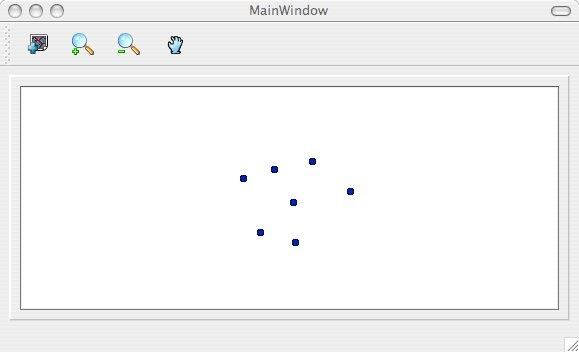
\includegraphics[clip=true, width=\textwidth]{cpp2_application}
\end{center}
\end{figure}

% \minisec{Conclusion}
\minisec{Conclusion}

% As you can see extending our previous example into something more functional
% using MapTools is really easy and only requires a few lines of code for each
% MapTool you want to provide.
Comme vous pouvez le voir, \'etendre notre exemple pr\'ec\'edent en quelque chose de 
plus fonctionnel en utilisant MapTools est vraiment facile et n\'ecessite 
seulement quelques lignes de codes pour chaque MapTool que vous voulez fournir.

% You can check out and build this tutorial using SVN and CMake using the following steps:
Vous pouvez r\'ecup\'erer et compiler ce tutoriel en utilisant SVN et CMake avec 
les \'etapes suivantes :

\begin{verbatim}
svn co https://svn.osgeo.org/qgis/trunk/code_examples/2_basic_main_window
cd 2_basic_main_window
mkdir build
#en option sp\'ecifiez o\`u QGIS est installe (doit fonctionner sur toutes les plateformes)
#si QGIS est installe dans /usr ou /usr/local vous pouvez laisser tomber l'\'etape suivante
export LIB_DIR=/home/timlinux/apps
cmake ..
make
./timtut2
\end{verbatim}

\section{Writing a QGIS Plugin in Python}

% when the revision of a section has been finalized,
% comment out the following line:
\updatedisclaimer

In this section you find a beginner's tutorial for writing a QGIS Python
plugins. It is based on the workshop "Extending the Functionality of QGIS
with Python Plugins" held at FOSS4G 2008 by Dr. Marco Hugentobler, Dr. Horst
D\"uster and Tim Sutton. 

Apart from writing a QGIS Python plugin, it is also possible to use PyQGIS
from a python command line console which is mainly interesting for debugging
or to write standalone applications in Python with their own user interfaces
using the functionality of the QGIS core library.

\subsection{Why Python and what about licensing}

Python is a scripting language which was designed with the goal of being easy
to program. It has a mechanism that automatically releases memory that is no
longer used (garbagge collector). A further advantage is that many programs
that are written in C++ or Java offer the possibility to write extensions in
Python, e.g. OpenOffice or Gimp. Therefore it is a good investment of time to
learn the Python language.

PyQGIS plugins use functionality of libqgis\_core.so and libqgis\_gui.so. As
both are licensed under GNU GPL, QGIS Python plugins must be licenced under the
GPL, too. This means you may use your plugins for any purpose and you are not
forced to publish them. If you do publish them however, they must be
published under the conditions of the GPL license. 

\subsection{What needs to be installed to get started}

On the lab computers, everything for the workshop is already installed. If
you program Python plugins at home, you will need the following libraries and
programs:

\begin{itemize}
\item QGIS
\item Python
\item Qt
\item PyQT
\item PyQt development tools
\end{itemize}

If you use Linux, there are binary packages for all major distributions. For
Windows, the PyQt installer already contains Qt, PyQt and the PyQt
development tools.

\subsection{Programming a simple PyQGIS Plugin in four steps}

The example plugin is intentionally kept simple. It adds a button to the menu
bar of QGIS. If the button is clicked, a file dialog appears where the user
may load a shape file.

For each python plugin, a dedicated folder that contains the plugin files
needs to be created. By default, QGIS looks for plugins in
\$QGIS\_DIR/share/qgis/python/plugins (in our workshop
/usr/share/qgis/python/plugins). On Linux, there is also the possibility to
have plugins in \$HOME/.qgis/python/plugins such that it is only visible for
one user.

\minisec{Step 1: Make the plugin manager recognise the plugin}

Each Python plugin is contained in its own directory. When QGIS starts up it
will scan each OS specific subdirectory and initialize any plugins it finds. 

\begin{itemize}
\item \nix{Linux and other unices}: ./share/qgis/python/plugins
\item \osx{Mac OS X}: ./Contents/MacOS/share/qgis/python/plugins
\item \win{Windows}: .\textbackslash share\textbackslash QGIS\textbackslash
python\textbackslash plugins
\end{itemize}

Once that's done, the plugin will show up in the
\dropmenuopttwo{mActionShowPluginManager}{Plugin Manager...}

\begin{Tip}\caption{\textsc{QGIS Python Plugin folder in \$HOME/.qgis}}
\qgistip{For Linux and other unices, there is also the possibility to have
your python plugins in \$HOME/.qgis/python/plugins. In that case, they are
only visible for one user.
}
\end{Tip}

To provide the neccessary information for QGIS, the plugin needs to implement
the methods \method{name()}, \method{description()} and \method{version()}
which return descriptive strings. A plugin also needs a method
\method{classFactory(QgisInterface)} which is called by the plugin manager to create
an instance of the plugin. The argument of type QGisInterface is used by the
plugin to access functions of the QGIS instance. We are going to work with
this object in step 2.  

Note that, in contrast to other programing languages, indention is very
important. The Python interpreter throws an error if it is not correct.

For our plugin we create the plugin folder 'foss4g\_plugin' in
\filename{./qgis/python/plugins}. Then we add two new textfiles into this
folder, \filename{foss4gplugin.py} and \filename{\_\_init\_\_.py}.

The file \filename{foss4gplugin.py} contains the plugin class:

\begin{verbatim}
# -*- coding: utf-8 -*-
# Import the PyQt and QGIS libraries
from PyQt4.QtCore import *
from PyQt4.QtGui import *
from qgis.core import *
# Initialize Qt resources from file resources.py
import resources

class FOSS4GPlugin:

def __init__(self, iface):
# Save reference to the QGIS interface
  self.iface = iface

def initGui(self):
  print 'Initialising GUI'

def unload(self):
  print 'Unloading plugin'
\end{verbatim}

The file \filename{\_\_init\_\_.py} contains the methods \method{name()},
\method{description()} and \method{version()} and \method{classFactory}. As
we are creating a new instance of the plugin class, we need to import the
code of this class:

\begin{verbatim}
# -*- coding: utf-8 -*-
from foss4gplugin import FOSS4GPlugin
def name():
  return "FOSS4G example"
def description():
  return "A simple example plugin to load shapefiles"
def version():
  return "Version 0.1"
def classFactory(iface):
  return FOSS4GPlugin(iface)
\end{verbatim}

At this point the plugin already the neccessary infrastructure to appear in
the QGIS \dropmenuopttwo{mActionShowPluginManager}{Plugin Manager...} to be
loaded or unloaded. 

\minisec{Step 2: Create an Icon for the plugin}

To make the icon graphic available for our program, we need a so-called
resource file. In the resource file, the graphic is contained in hexadecimal
notation. Fortunately, we don't need to care about its representation because
we use the pyrcc compiler, a tool that reads the file
\filename{resources.qrc} and creates a resource file. 

The file \filename{foss4g.png} and the \filename{resources.qrc} we use in
this little workshop can be downloaded from
\url{http://karlinapp.ethz.ch/python\_foss4g}. Move these 2 files into the
directory of the example plugin
\filename{./qgis/python/plugins/foss4g\_plugin} and enter: <path\_to\_QGIS\_folder>/pyrcc4 -o
resources.py resources.qrc.

\minisec{Step 3: Add a button and a menu}

In this section, we implement the content of the methods \method{initGui()} and
\method{unload()}. We need an instance of the class \classname{QAction} that executes the
\method{run()} method of the plugin. With the action object, we are then able to
generate the menu entry and the button:

\begin{verbatim}
import resources

  def initGui(self):
    # Create action that will start plugin configuration
    self.action = QAction(QIcon(":/plugins/foss4g_plugin/foss4g.png"), "FOSS4G plugin",
self.iface.getMainWindow())
    # connect the action to the run method
    QObject.connect(self.action, SIGNAL("activated()"), self.run)

    # Add toolbar button and menu item
    self.iface.addToolBarIcon(self.action)
    self.iface.addPluginMenu("FOSS-GIS plugin...", self.action)

    def unload(self):
    # Remove the plugin menu item and icon
    self.iface.removePluginMenu("FOSSGIS Plugin...", self.action)
    self.iface.removeToolBarIcon(self.action)
\end{verbatim}

\minisec{Step 4: Load a layer from a shape file}

In this step we implement the real functionality of the plugin in the
\method{run()} method. The Qt4 method \method{QFileDialog::getOpenFileName}
opens a file dialog and returns the path to the chosen file. If the user
cancels the dialog, the path is a null object, which we test for. We then
call the method \method{addVectorLayer} of the interface object which loads
the layer. The method only needs three arguments: the file path, the name of
the layer that will be shown in the legend and the data provider name. For
shapefiles, this is 'ogr' because QGIS internally uses the OGR library to
access shapefiles:

\begin{verbatim}
    def run(self):
    fileName = QFileDialog.getOpenFileName(None,QString.fromLocal8Bit("Select a file:"),
 "", "*.shp *.gml")
    if fileName.isNull():
      QMessageBox.information(None, "Cancel", "File selection canceled")
      else:
      vlayer = self.iface.addVectorLayer(fileName, "myLayer", "ogr")
\end{verbatim}

\subsection{Further information}

As you can see, you need information from different sources to write PyQGIS
plugins. Plugin writers need to know Python and the QGIS plugin interface as
well as the Qt4 classes and tools. At the beginning it is best to learn from
examples and copy the mechanism of existing plugins. Using the QGIS plugin
installer, which itself is a Python plugin, it is possible to download a lot
of existing Python plugins and to study their behaviour.

There is a a collection of online documentation that may be usefull for
PyQGIS programers:
 
\begin{itemize}
\item QGIS wiki: \url{http://wiki.qgis.org/qgiswiki/PythonBindings}
\item QGIS API documentation: \url{http://doc.qgis.org/index.html}
\item Qt documentation: \url{http://doc.trolltech.com/4.3/index.html}
\item PyQt: \url{http://www.riverbankcomputing.co.uk/pyqt/}
\item Python tutorial: \url{http://docs.python.org/}
\item A book about desktop GIS and QGIS. It contains a chapter about PyQGIS
plugin programing: \url{http://www.pragprog.com/titles/gsdgis/desktop-gis} 
\end{itemize}

You can also write plugins for QGIS in C++. See Section \ref{cpp_plugin} for
more information about that.


% vim: set textwidth=78 autoindent:

\section{Creating PyQGIS Applications}

% when the revision of a section has been finalized, 
% comment out the following line:
% \updatedisclaimer

One of the goals of QGIS is to provide not only an application, but a set of
libraries that can be used to create new applications. This goal has been
realized with the refactoring of libraries that took place after the release
of 0.8. Since the release of 0.9, development of standalone applications using
either C++ or Python is possible. We recommend you use QGIS 1.0.0 or greater
as the basis for your pythong applications because since this version we now
provide a stable consistent API.

In this chapter we'll take a brief look at the process for creating a
standalone Python application. The QGIS blog has several examples of creating
PyQGIS\footnote{An application created using Python and the QGIS bindings}
applications. We'll use one of them as a starting point to get a look at how
to create an application.

The features we want in the application are:

\begin{itemize}
\item Load a vector layer
\item Pan
\item Zoom in and out
\item Zoom to the full extent of the layer
\item Set custom colors when the layer is loaded
\end{itemize} 

This is a pretty minimal feature set. Let's start by designing the GUI using
Qt Designer. 

\subsection{Designing the GUI}

Since we are creating a minimalistic application, we'll take the same
approach with the GUI. Using Qt Designer, we create a simple MainWindow with
no menu or toolbars. This gives us a blank slate to work with. To create the
MainWindow:

\begin{enumerate}
\item Create a directory for developing the application and change to it
\item Run Qt Designer
\item The \qtdialog{New Form} dialog should appear. If it doesn't, choose
\qtdropmenuopt{New Form...} from the \qtmainmenuopt{File} menu.
\item Choose \qtdropmenuopt{Main Window} from 
the \qtdropmenuopt{templates/forms} list
\item Click \qtdropmenuopt{Create} 
\item Resize the new window to something manageable
\item Find the \qtdropmenuopt{Frame} widget in the list 
(under \qtdropmenuopt{Containers}) and drag it to
the main window you just created
\item Click outside the frame to select the main window area 
\item Click on the \qtdropmenuopt{Lay Out in a Grid} tool. When you do, the frame
will expand to fill your entire main window
\item Save the form as \usertext{mainwindow.ui} 
\item \qtdropmenuopt{Exit} Qt Designer
\end{enumerate} 

Now compile the form using the PyQt interface compiler:

\begin{verbatim}
   pyuic4 -o mainwindow_ui.py mainwindow.ui
\end{verbatim}

This creates the Python source for the main window GUI. Next we need to create
the application code to fill the blank slate with some tools we can use.

\subsection{Creating the MainWindow}

Now we are ready to write the \classname{MainWindow} class that will do the real work.
Since it takes up quite a few lines, we'll look at it in chunks, starting
with the import section and environment setup:

\begin{verbatim}
1 # Loosely based on:
2 #   Original C++ Tutorial 2 by Tim Sutton
3 #   ported to Python by Martin Dobias
4 #   with enhancements by Gary Sherman for FOSS4G2007
5 # Licensed under the terms of GNU GPL 2
6
7 from PyQt4.QtCore import *
8 from PyQt4.QtGui import *
9 from qgis.core import *
10 from qgis.gui import *
11 import sys
12 import os
13 # Import our GUI
14 from mainwindow_ui import Ui_MainWindow
15 
16 # Environment variable QGISHOME must be set to the 1.0 install directory
17 # before running this application
18 qgis_prefix = os.getenv("QGISHOME")
\end{verbatim}

Some of this should look familiar from our plugin, especially the PyQt4 and
QGIS imports. Some specific things to note are the import of our GUI in line
14 and the import of our CORE library on line 9.

Our application needs to know where to find the QGIS installation. Because
of this, we set the \usertext{QGISHOME} environment variable to point to the 
install directory of QGIS 1.x In line 20 we store this value from
the environment for later use.

Next we need to create our \classname{MainWindow} class which will contain
all the logic of our application.
\begin{verbatim}
21 class MainWindow(QMainWindow, Ui_MainWindow):
22 
23   def __init__(self):
24     QMainWindow.__init__(self)
25 
26     # Required by Qt4 to initialize the UI
27     self.setupUi(self)
28 
29     # Set the title for the app
30     self.setWindowTitle("QGIS Demo App")
31 
32     # Create the map canvas
33     self.canvas = QgsMapCanvas()
34     # Set the background color to light blue something
35     self.canvas.setCanvasColor(QColor(200,200,255))
36     self.canvas.enableAntiAliasing(True)
37     self.canvas.useQImageToRender(False)
38     self.canvas.show()
39 
40     # Lay our widgets out in the main window using a 
41     # vertical box layout
42     self.layout = QVBoxLayout(self.frame)
43     self.layout.addWidget(self.canvas)
44 
45     # Create the actions for our tools and connect each to the appropriate
46     # method
47     self.actionAddLayer = QAction(QIcon("(qgis_prefix + "/share/qgis/themes/classic/mActionAddLayer.png"),
48     \
49         "Add Layer", self.frame)
50     self.connect(self.actionAddLayer, SIGNAL("activated()"), self.addLayer)
51     self.actionZoomIn = QAction(QIcon("(qgis_prefix + "/share/qgis/themes/classic/mActionZoomIn.png"), \
52         "Zoom In", self.frame)
53     self.connect(self.actionZoomIn, SIGNAL("activated()"), self.zoomIn)
54     self.actionZoomOut = QAction(QIcon("(qgis_prefix + "/share/qgis/themes/classic/mActionZoomOut.png"), \
55         "Zoom Out", self.frame)
56     self.connect(self.actionZoomOut, SIGNAL("activated()"), self.zoomOut)
57     self.actionPan = QAction(QIcon("(qgis_prefix + "/share/qgis/themes/classic/mActionPan.png"), \
58         "Pan", self.frame)
59     self.connect(self.actionPan, SIGNAL("activated()"), self.pan)
60     self.actionZoomFull = QAction(QIcon("(qgis_prefix + "/share/qgis/themes/classic/mActionZoomFullExtent.png"), \
61         "Zoom Full Extent", self.frame)
62     self.connect(self.actionZoomFull, SIGNAL("activated()"),
63     self.zoomFull)
64 
65     # Create a toolbar
66     self.toolbar = self.addToolBar("Map")
67     # Add the actions to the toolbar
68     self.toolbar.addAction(self.actionAddLayer)
69     self.toolbar.addAction(self.actionZoomIn)
70     self.toolbar.addAction(self.actionZoomOut);
71     self.toolbar.addAction(self.actionPan);
72     self.toolbar.addAction(self.actionZoomFull);
73 
74     # Create the map tools
75     self.toolPan = QgsMapToolPan(self.canvas)
76     self.toolZoomIn = QgsMapToolZoom(self.canvas, False) # false = in
77     self.toolZoomOut = QgsMapToolZoom(self.canvas, True) # true = out
\end{verbatim}

Lines 21 through 27 are the basic declaration and initialization of the 
\classname{MainWindow} and the set up of the user interface using the 
\method{setupUi} method. This is required for all applications.

Next we set the title for the application so it says something more
interesting than \usertext{MainWindow} (line 30). Once that is
complete, we are ready to complete the user interface. When we created it in
Designer, we left it very sparse---just a main window and a frame. You could
have added a menu and the toolbar using Designer, however we'll do it with
Python.

In lines 33 through 38 we set up the map canvas, set the background color to a
light blue, and enable antialiasing.  We also tell it not to use a
\classname{QImage} for rendering (trust me on this one) and then set the
canvas to visible by calling the \method{show} method.

Next we set the layer to use a vertical box layout within the frame and add
the map canvas to it in line 43.

Lines 48 to 63 set up the actions and connections for the tools in our
toolbar. For each tool, we create a \classname{QAction} using the icon we
defined in the QGIS classic theme.  Then we connect up the
\usertext{activated} signal from the tool to the method in our class that will
handle the action. This is similar to how we set things up in the plugin
example.

Once we have the actions and connections, we need to add them to the toolbar.
In lines 66 through 72 we create the toolbar and add each tool to it.

Lastly we create the three map tools for the application (lines 75 through
77). We'll use the map tools in a moment when we define the methods to make
our application functional. Let's look at the methods for the map tools.

\begin{verbatim}
78   # Set the map tool to zoom in
79   def zoomIn(self):
80     self.canvas.setMapTool(self.toolZoomIn)
81 
82   # Set the map tool to zoom out
83   def zoomOut(self):
84     self.canvas.setMapTool(self.toolZoomOut)
85 
86   # Set the map tool to 
87   def pan(self):
88    self.canvas.setMapTool(self.toolPan)
89 
90   # Zoom to full extent of layer
91   def zoomFull(self):
92     self.canvas.zoomFullExtent()
\end{verbatim}

For each map tool, we need a method that corresponds to the connection we made
for each action. In lines 79 through 88 we set up a method for each of the
  three tools that interact with the map. When a tool is activated by clicking
  on it in the toolbar, the corresponding method is called that ``tells'' the
  map canvas it is the active tool. The active tool governs what happens when
  the mouse is clicked on the canvas.

The \usertext{zoom to full extent} tool isn't a map tool---it does its job
without requiring a click on the map. When it is activated, we call the
\method{zoomFullExtent} method of the map canvas (line 92).  This completes
the implementation of all our tools except one---the \usertext{Add Layer}
tool. %FIXME 
Let's look at it next:

\begin{verbatim}
93   # Add an OGR layer to the map
94   def addLayer(self):
95     file = QFileDialog.getOpenFileName(self, "Open Shapefile", ".", "Shapefiles
96     (*.shp)")
97     fileInfo = QFileInfo(file)
98 
99     # Add the layer
100     layer = QgsVectorLayer(file, fileInfo.fileName(), "ogr")
101
102    if not layer.isValid():
103      return
104
105    # Change the color of the layer to gray
106    symbols = layer.renderer().symbols()
107    symbol = symbols[0]
108    symbol.setFillColor(QColor.fromRgb(192,192,192))
109
110    # Add layer to the registry
111    QgsMapLayerRegistry.instance().addMapLayer(layer);
112
113    # Set extent to the extent of our layer
114    self.canvas.setExtent(layer.extent())
115
116    # Set up the map canvas layer set
117    cl = QgsMapCanvasLayer(layer)
118    layers = [cl]
119    self.canvas.setLayerSet(layers)
\end{verbatim}

In the \method{addLayer} method we use a \classname{QFileDialog} to get the
name of the shapefile to load. This is done in line 96.
Notice that we specify a ``filter'' so the dialog will only show files of
type \filename{.shp}.

Next in line 97 we create a \classname{QFileInfo} object from the shapefile
path.  Now the layer is ready to be created in line 100. Using the
\classname{QFileInfo} object to get the file name from the path we specify it 
for the name of the layer when it is created.  To make sure that the layer is 
valid and won't cause any problems when loading, we check it in line 102. If
it's bad, we bail out and don't add it to the map canvas.

Normally layers are added with a random color. Here we want to tweak the
colors for the layer to make a more pleasing display. Plus we know we are
going to add the \filename{world\_borders} layer to the map and this will make
it look nice on our blue background. To change the color, we need to get the
symbol used for rendering and use it to set a new fill color. This is done in
lines 106 through 108. 

All that's left is to actually add the layer to the registry and a few other
housekeeping items (lines 111 through 119). This stuff is standard for adding
a layer and the end result is the world borders on a light blue background.
The only thing you may not want to do is set the extent to the layer, if you
are going to be adding more than one layer in your application.

That's the heart of the application and completes the \classname{MainWindow} class. 

\subsection{Finishing Up}

The remainder of the code shown below creates the \object{QgsApplication}
object, sets the path to the QGIS install, sets up the \method{main} method
and then starts the application. The only other thing to note is that we move
the application window to the upper left of the display. We could get fancy
and use the Qt API to center it on the screen.

\begin{verbatim}
120 def main(argv):
121   # create Qt application
122   app = QApplication(argv)
123 
124   # Initialize qgis libraries
125   QgsApplication.setPrefixPath(qgis_prefix, True)
126   QgsApplication.initQgis()
127 
128   # create main window
129   wnd = MainWindow()
130   # Move the app window to upper left
131   wnd.move(100,100)
132   wnd.show()
133 
134   # run!
135   retval = app.exec_()
136   
137   # exit
138   QgsApplication.exitQgis()
139   sys.exit(retval)
140 
141 
142 if __name__ == "__main__":
143   main(sys.argv)
\end{verbatim}

\subsection{Running the Application}

Now we can run the application and see what happens. Of course if you are like 
most developers, you've been testing it out as you went along. 

Before we can run the application, we need to set some environment variables. 

\nix{}\osx{}
\begin{verbatim}
export LD_LIBRARY_PATH=$HOME/qgis/lib%$
export PYTHONPATH=$HOME/qgis/share/qgis/python
export QGISHOME=$HOME/qgis%$
\end{verbatim}

\win{}
\begin{verbatim}
set PATH=C:\qgis;%PATH%
set PYTHONPATH=C:\qgis\python
set QGISHOME=C:\qgis
\end{verbatim}

We assume
\begin{itemize}
\item\nix{}\osx{}QGIS is installed in 
your home directory in 
\filename{qgis}. 
\item\win{}QGIS is installed in \filename{C:\textbackslash qgis}.
\end{itemize}

When the application starts up, it looks like this:

%\begin{figure}[ht]
%\begin{center}
%  \caption{Starting the new demo application}\label{fig:demo_app_startup}%\smallskip
%  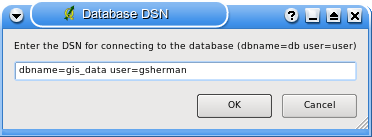
\includegraphics[scale=0.8]{getdsn}
%\end{center}
%\end{figure}

To add the \filename{world\_borders} layer, click on the 
\usertext{Add Layer} tool and navigate to the data directory.
Select the shapefile and click \button{Open} to add it to the map. 
Our custom fill color is applied and the result is:

%\begin{figure}[ht]
%\begin{center}
%  \caption{Adding a layer the demo application}\label{fig:demo_app_done}%\smallskip
%  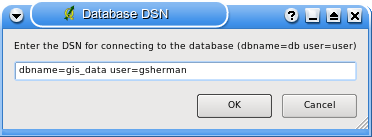
\includegraphics[scale=0.8]{getdsn}
%\end{center}
%\end{figure}

Creating a PyQGIS application is really pretty simple.  In less than 150 lines
of code we have an application that can load a shapefile and navigate the map.
If you play around with the map, you'll notice that some of the built-in
features of the canvas also work, including mouse wheel scrolling and panning
by holding down the \keystroke{Space} bar and moving the mouse.

Some sophisticated applications have been created with PyQGIS and more are in 
the works. This is pretty impressive, considering that this development has 
taken place even before the official release of QGIS 1.0.

\begin{Tip}\caption{\textsc{Documentation For PyQGIS}}
\qgistip{Whether you are writing a plugin or a PyQGIS application, you are
going to need to refer to both the QGIS API documentation
(\url{http://doc.qgis.org}) and the PyQt Python Bindings Reference Guide
(\url{http://www.riverbankcomputing.com/Docs/PyQt4/pyqt4ref.html}). These
documents provide information about the classes and methods you'll use to
bring your Python creation to life.
}
\end{Tip} 

% \section{Help and Support}\label{label_helpsupport}
\section{Aide et support}\label{label_helpsupport}

% when the revision of a section has been finalized, 
% comment out the following line:
% \updatedisclaimer

\subsection{Mailinglists}
% QGIS is under active development and as such it won't always work like
% you expect it to. The preferred way to get help is by joining the qgis-users
% mailing list.
QGIS est en cours de développement par conséquent il ne fonctionne pas toujours
comme attendu. La manière préférée d'obtenir de l'aide est de rejoindre la
liste de diffusion qgis-users.

\minisec{qgis-users}
% Your questions will reach a broader audience and answers will
% benefit others. You can subscribe to the qgis-users mailing list by visiting
% the following URL: \\
% \url{http://lists.osgeo.org/mailman/listinfo/qgis-user}
Vos questions atteindront une audience plus large et les réponses bénéficieront
à tous. Vous pouvez rejoindre la liste de diffusion qgis-users en allant sur la
page suivante : \\
\url{http://lists.osgeo.org/mailman/listinfo/qgis-user}

\minisec{qgis-developer}
% If you are a developer facing problems of a more technical nature, you may
% want to join the qgis-developer mailing list here:\\
% \url{http://lists.osgeo.org/mailman/listinfo/qgis-developer}
Si vous êtes un développeur et que vous faites face à un problème plus
technique, vous pourrez préférer rejoindre la liste de diffusion qgis-developer
ici :\\
\url{http://lists.osgeo.org/mailman/listinfo/qgis-developer}

\minisec{qgis-commit}
% Each time a commit is made to the QGIS code repository an email is posted to
% this list. If you want to be up to date with every change to the current code
% base, you can subscribe to this list at:\\
% \url{http://lists.osgeo.org/mailman/listinfo/qgis-commit}
À chaque fois qu'un commit est réalisé sur le dépôt du code de QGIS un email
est envoyé à cette liste. Si vous voulez être à jour de chaque changement au
code en cours, vous pouvez vous inscrire à cette liste :\\
\url{http://lists.osgeo.org/mailman/listinfo/qgis-commit}

\minisec{qgis-trac}
% This list provides email notification related to project management,
% including bug reports, tasks, and feature requests. You can subscribe to this
% list at:\\
% \url{http://lists.osgeo.org/mailman/listinfo/qgis-trac}
Cette liste fournit une notification par mail liée à la gestion du projet,
incluant les rapports de bugs, tâches, et demande de fonctionnalités. Vous
pouvez vous inscrire à cette liste ici :\\
\url{http://lists.osgeo.org/mailman/listinfo/qgis-trac}

\minisec{qgis-community-team}
% This list deals with topics like documentation, context help, user-guide,
% online experience including web sites, blog, mailing lists, forums, and
% translation efforts. If you like to work on the user-guide as well, this list
% is a good starting point to ask your questions. You can subscribe to this
% list at:\\
% \url{http://lists.osgeo.org/mailman/listinfo/qgis-community-team}
Cette liste reçoit les mails des thématiques lié à la documentation, au
contexte d'aide, au guide utilisateur, à ce qui est lié à Internet donc les
sites, listes de diffusion, forums et efforts de traduction. Si vous voulez
travailler sur le guide utilisateur, cette liste est un bon point de départ
pour poser vos questions. Vous pouvez vous inscrire à cette liste ici :\\
\url{http://lists.osgeo.org/mailman/listinfo/qgis-community-team}

\minisec{qgis-release-team}
% This list deals with topics like the release process, packaging binaries for
% various OS and announcing new releases to the world at large. You can
% subscribe to this list at:\\
% \url{http://lists.osgeo.org/mailman/listinfo/qgis-release-team}
Cette liste reçoit les mails des thématiques comme les procédures de
publication de version, paquetage binaire pour différents systèmes et annonce
des nouvelles versions à un monde plus large. Vous pouvez vous inscrire à cette
liste ici :\\
\url{http://lists.osgeo.org/mailman/listinfo/qgis-release-team}

\minisec{qgis-psc}
% This list is used to discuss Steering Committee issues related to overall
% management and direction of Quantum GIS. You can subscribe to this list at:\\
% \url{http://lists.osgeo.org/mailman/listinfo/qgis-psc}
Cette liste est utilisée pour discuter des problèmes du Comité de Pilotage lié à
l'ensemble de la gestion et de la direction de Quantum GIS. Vous pouvez vous
inscrire à cette liste ici :\\
\url{http://lists.osgeo.org/mailman/listinfo/qgis-psc}

% You are welcome to subscribe to any of the lists. Please remember to
% contribute to the list by answering questions and sharing your experiences.
% Note that the qgis-commit and qgis-trac are designed for notification only
% and not meant for user postings.
Vous êtes invité à vous inscrire à ces listes. S'il vous plait, souvenez-vous de
contribuer à la liste en répondant à des questions et en partageant vos
expériences. Remarquez que les listes qgis-commit et qgis-trac ont été
configurées pour notification seulement et n'acceptent pas de mail
d'utilisateurs.

\subsection{IRC}
% We also maintain a presence on IRC - visit us by joining the \#qgis channel on
% \url{irc.freenode.net}. Please wait around for a response to your question as
% many folks on the channel are doing other things and it may take a while for
% them to notice your question. Commercial support for QGIS is also available.
% Check the website \url{http://qgis.org/content/view/90/91} for more
% information.
Nous maintenons une présence sur IRC - rejoignez-nous sur le canal \#qgis sur
\url{irc.freenode.net}. S'il vous plait, patientez pour obtenir une réponse
puisque la plupart des personnes font autre chose et cela peut leur prendre un
peu de temps pour remarquer votre question. Un support commercial pour QGIS est
disponible. Regardez la page du site \url{http://qgis.org/content/view/90/91}
pour plus d'informations.

% If you missed a discussion on IRC, not a problem! We log all discussion so you
% can easily catch up. Just go to \url{http://logs.qgis.org} and read the
% IRC-logs.
Si vous ratez une discussion sur IRC, pas de problème ! Nous loguons toutes les
discussions afin que vous puisiez facilement les suivre. Allez simplement sur
\url{http://logs.qgis.org} et lisez les logs IRC.

\subsection{BugTracker}
% While the qgis-users mailing list is useful for general 'how do I do xyz in
% QGIS' type questions, you may wish to notify us about bugs in QGIS. You can
% submit bug reports using the QGIS bug tracker at
% \url{https://trac.osgeo.org/qgis/}. When creating a new ticket for a bug,
% please provide an email address where we can request additional information.
Bien que la liste de diffusion utilisateur est utile pour des questions
générales du type 'Comment je réalise xyz dans QGIS ?', vous pouvez vouloir
nous avertir de bugs dans QGIS. Vous pouvez soumettre un rapport de bug en
utilisant le tracker de bug sur \url{https://trac.osgeo.org/qgis/}. Lors de la
création d'un ticket pour un bug, fournissez s'il vous plait une adresse mail
valide où nous pouvons vous demander des informations supplémentaires.

% Please bear in mind that your bug may not always enjoy the priority you might
% hope for (depending on its severity). Some bugs may require significant
% developer effort to remedy and the manpower is not always available for this.
Garder en mémoire que votre bug peut ne pas avoir la priorité à laquelle vous
vous attendiez (cela dépendra de sa sévérité). Certains bugs peuvent nécessiter du
travail supplémentaire de la part des développeurs pour y remédier et la personne
compétente n'est pas forcément disponible.

% Feature requests can be submitted as well using the same ticket system as for
% bugs. Please make sure to select the type \usertext{enhancement}.
Les demandes de fonctionnalité peuvent être soumises également en utilisant le
même système de ticket que pour les bugs. Assurez-vous de sélectionner le type
\usertext{enhancement}.

% If you have found a bug and fixed it yourself you can submit this patch also.
% Again, the lovely trac ticketsystem at \url{https://trac.osgeo.org/qgis/} has
% this type as well. Select \usertext{patch} from the type-menu. Someone of the 
% developers will review it and apply it to QGIS. \\
Si vous avez trouvé un bug et l'avez corrigé vous même, vous pouvez
aussi soumettre un patch. Encore, le superbe système de ticket Trac sur
\url{https://trac.osgeo.org/qgis/} a également ce type. Sélectionnez
\usertext{patch} dans le menu type. Un des développeurs le vérifiera et
l'appliquera à QGIS.\\
% Please don't be alarmed if your patch is not applied straight away -
% developers may be tied up with other committments.
Ne vous alarmez pas si votre correctif n'est pas appliqué directement - les
développeurs peuvent être occupés sur d'autres commits.

% unused, since community.qgis.org seems to be lost. (SH)
% There is also a community site for QGIS where we encourage QGIS users to share
% their experiences and provide case studies about how they are using QGIS. The
% community site is available at: http://community.qgis.org 

\subsection{Blog}
% The QGIS-community also runs a weblog (BLOG) at \url{http://blog.qgis.org} 
% which has some interesting articles for users and developers as well. 
% You are invited to contribute to the blog after registering yourself!
La communauté QGIS tient également un weblog (BLOG) sur
\url{http://blog.qgis.org} qui publie d'intéressants articles à la fois pour les
utilisateurs et les développeurs. Vous êtes invités à contribuer au blog après
vous être enregistrés.

\subsection{Wiki}
% Lastly, we maintain a WIKI web site at \url{http://wiki.qgis.org} where you 
% can find a variety of useful information relating to QGIS development, 
% release plans, links to download sites, message translation-hints and so
% on. Check it out, there are some goodies inside!
Enfin, nous maintenons un site web wiki sur \url{http://wiki.qgis.org} où vous
pouvez trouver diverses informations utiles liées au développement de QGIS, plan
des versions, liens vers les sites de téléchargement, astuces de
traduction des messages, etc. Parcourez le, il y a des choses intéressantes.

%install and coding guide is a special case because we are extracting it
%out of the INSTALL.t2t and CODING.t2t document of in the QGIS sources
%when we tag a new document release
\section{Installation Guide}

The following chapters provide build and installation information for QGIS 
Version \CURRENT. This document corresponds almost to a \LaTeX~ conversion of 
the INSTALL.t2t file coming with the QGIS sources from November, 29th 2007.

A current version is also available at the wiki, see:
\htmladdnormallink{http://wiki.qgis.org/qgiswiki/BuildingFromSource}{http://wiki.qgis.org/qgiswiki/BuildingFromSource} 

\subsection{General Build Notes}

At version 0.8.1 QGIS no longer uses the autotools for building. QGIS, like a
number of major projects (eg. KDE 4.0), now uses cmake for building from
source. The configure script in this directory simply checks for the existence
of cmake and provides some clues to build QGIS.

For complete information, see the wiki at:
   \htmladdnormallink{http://wiki.qgis.org/qgiswiki/Building\_with\_CMake}{http://wiki.qgis.org/qgiswiki/Building\_with\_CMake}

\subsection{An overview of the dependencies required for building}

\textbf{Required build deps:}

\begin {itemize}
\item CMake $>$= 2.4.3
\item Flex, Bison
\end{itemize}

\textbf{Required runtime deps:}

\begin {itemize}
\item Qt $>$= 4.2.0
\item Proj $>$= ? (known to work with 4.4.x)
\item GEOS $>$= 2.2 (3.0 is supported, maybe 2.1.x works too)
\item Sqlite3 $>$= ? (probably 3.0.0)
\item GDAL/OGR $>$= ? (1.2.x should work)
\end{itemize}

\textbf{Optional dependencies:}

\begin {itemize}
\item for GRASS plugin - GRASS $>$= 6.0.0
\item for georeferencer - GSL $>$= ? (works with 1.8)
\item for postgis support and SPIT plugin - PostgreSQL $>$= ?
\item for gps plugin - expat $>$= ? (1.95 is OK)
\item for mapserver export and PyQGIS - Python $>$= ? (probably 2.3)
\item for PyQGIS - SIP $>$= 4.5, PyQt $>$= 4.1
\end{itemize}

\textbf{Recommended runtime deps:}

\begin {itemize}
\item for gps plugin - gpsbabel
\end{itemize}

\section{Building under windows using msys}\label{sec:install_windows}
\subsection{MSYS:}
MSYS provides a unix style build environment under windows. We have created a
zip archive that contains just about all dependencies.

Get this: 

\htmladdnormallink{http://qgis.org/uploadfiles/msys/msys.zip}{http://qgis.org/uploadfiles/msys/msys.zip}

and unpack to c:$\backslash$msys

If you wish to prepare your msys environment yourself rather than using 
our pre-made one, detailed instructions are provided elsewhere in this
document.

\subsection{Qt4.3}
Download qt4.3 opensource precompiled edition exe and install (including the
download and install of mingw) from here:

\htmladdnormallink{http://www.trolltech.com/developer/downloads/qt/windows}{http://www.trolltech.com/developer/downloads/qt/windows}

When the installer will ask for MinGW, you don't need to download and install
it, just point the installer to c:$\backslash$msys$\backslash$mingw

When Qt installation is complete:

Edit C:$\backslash$Qt$\backslash$4.3.0$\backslash$bin$\backslash$qtvars.bat and add the following lines:

\begin{verbatim}
set PATH=%PATH%;C:\msys\local\bin;c:\msys\local\lib 
set PATH=%PATH%;"C:\Program Files\Subversion\bin" 
\end{verbatim}

I suggest you also add C:$\backslash$Qt$\backslash$4.3.0$\backslash$bin$\backslash$ to your Environment Variables Path in
the windows system preferences.

If you plan to do some debugging, you'll need to compile debug version of Qt:
C:$\backslash$Qt$\backslash$4.3.0$\backslash$bin$\backslash$qtvars.bat compile\_debug

Note: there is a problem when compiling debug version of Qt 4.3, the script ends with
this message  "mingw32-make: *** No rule to make target `debug'.  Stop.". To 
compile the debug version you have to go out of src directory and execute the
following command:

\begin{verbatim}
c:\Qt\4.3.0 make 
\end{verbatim}

\subsection{Flex and Bison}
*** Note I think this section can be removed as it should be installed int the
msys image already. TS

Get Flex
\htmladdnormallink{http://sourceforge.net/project/showfiles.php?group\_id=23617\&package\_id=16424}{http://sourceforge.net/project/showfiles.php?group\_id=23617\&package\_id=16424}
(the zip bin) and extract it into c:$\backslash$msys$\backslash$mingw$\backslash$bin

\subsection{Python stuff: (optional)}
Follow this section in case you would like to use Python bindings for QGIS.  To
be able to compile bindings, you need to compile SIP and PyQt4 from sources as
their installer doesn't include some development files which are necessary.

\subsubsection{Download and install Python - use Windows installer}
(It doesn't matter to what folder you'll install it)

\htmladdnormallink{http://python.org/download/}{http://python.org/download/}

\subsubsection{Download SIP and PyQt4 sources}

\begin{verbatim}
\htmladdnormallink{http://www.riverbankcomputing.com/Downloads/sip4/}
\htmladdnormallink{http://www.riverbankcomputing.com/Downloads/PyQt4/GPL/}
\end{verbatim}

Extract each of the above zip files in a temporary directory. Make sure
to get versions that match your current Qt installed version.

\subsubsection{Compile SIP}
\begin{verbatim}
c:\Qt\4.3.0\bin\qtvars.bat 
python configure.py -p win32-g++ 
make 
make install 
\end{verbatim}

\subsubsection{Compile PyQt}
\begin{verbatim}
c:\Qt\4.3.0\bin\qtvars.bat 
python configure.py 
make 
make install 
\end{verbatim}

\subsubsection{Final python notes}
/!$\backslash$ You can delete the directories with unpacked SIP and PyQt4 sources after a
successfull install, they're not needed anymore.

\subsection{Subversion:}
In order to check out QGIS sources from the repository, you need Subversion
client. This installer should work fine:

\htmladdnormallink{http://subversion.tigris.org/files/documents/15/36797/svn-1.4.3-setup.exe}{http://subversion.tigris.org/files/documents/15/36797/svn-1.4.3-setup.exe}

\subsection{CMake:}
CMake is build system used by Quantum GIS. Download it from here:

\htmladdnormallink{http://www.cmake.org/files/v2.4/cmake-2.4.6-win32-x86.exe}{http://www.cmake.org/files/v2.4/cmake-2.4.6-win32-x86.exe}

\subsection{QGIS:}
Start a cmd.exe window ( Start -$>$ Run -$>$ cmd.exe ) Create development 
directory and move into it

\begin{verbatim}
md c:\dev\cpp 
cd c:\dev\cpp 
\end{verbatim}

Check out sources from SVN For svn head:

\begin{verbatim}
svn co https://svn.qgis.org/repos/qgis/trunk/qgis 
\end{verbatim}
For svn 0.8 branch

\begin{verbatim}
 svn co https://svn.qgis.org/repos/qgis/branches/Release-0_8_0 qgis0.8
\end{verbatim}

\subsection{Compiling:}
As a background read the generic building with CMake notes at the end of 
this document.

Start a cmd.exe window ( Start -$>$ Run -$>$ cmd.exe ) if you don't have one
already.  Add paths to compiler and our MSYS environment:

\begin{verbatim}
c:\Qt\4.3.0\bin\qtvars.bat 
\end{verbatim}

For ease of use add c:$\backslash$Qt$\backslash$4.3.0$\backslash$bin$\backslash$ to your system path in system
properties so you can just type qtvars.bat when you open the cmd console.
Create build directory and set it as current directory:

\begin{verbatim}
cd c:\dev\cpp\qgis 
md build 
cd build 
\end{verbatim}

\subsection{Configuration}
\begin{verbatim}
cmakesetup ..  
\end{verbatim}

\textbf{NOTE}: You must include the '..' above.

Click 'Configure' button.  When asked, you should choose 'MinGW Makefiles'
as generator.

There's a problem with MinGW Makefiles on Win2K. If you're compiling on this
platform, use 'MSYS Makefiles' generator instead.

All dependencies should be picked up automatically, if you have set up the
Paths correctly. The only thing you need to change is the installation
destination (CMAKE\_INSTALL\_PREFIX) and/or set 'Debug'.

For compatibility with NSIS packaging cripts I recommend to leave the
install prefix to its default c:$\backslash$program files$\backslash$

When configuration is done, click 'OK' to exit the setup utility.

\subsection{Compilation and installation}
\begin{verbatim}
make 
make install 
\end{verbatim}

\subsection{Run qgis.exe from the directory where it's installed (CMAKE\_INSTALL\_PREFIX)}
Make sure to copy all .dll:s needed to the same directory as the qgis.exe
binary is installed to, if not already done so, otherwise QGIS will complain
about missing libraries when started.

The best way to do this is to download both the QGIS current release installer
package from \htmladdnormallink{http://qgis.org/uploadfiles/testbuilds/}{http://qgis.org/uploadfiles/testbuilds/} and install it. Now copy
the installation dir from C:$\backslash$Program Files$\backslash$Quantum GIS into c:$\backslash$Program
Files$\backslash$qgis-0.8.1 (or whatever the current version is. The name should strictly
match the version no.) After making this copy you can uninstall the release
version of QGIS from your c:$\backslash$Program Files directory using the provided
uninstaller. Double check that the Quantum GIS dir is completely gone under
program files afterwards.

Another possibility is to run qgis.exe when your path contains
c:$\backslash$msys$\backslash$local$\backslash$bin and c:$\backslash$msys$\backslash$local$\backslash$lib directories, so the DLLs will be
used from that place.

\subsection{Create the installation package: (optional)}
Downlad and install NSIS from (\htmladdnormallink{http://nsis.sourceforge.net/Main\_Page}{http://nsis.sourceforge.net/Main\_Page})

Now using windows explorer, enter the win\_build directory in your QGIS source
tree. Read the READMEfile there and follow the instructions. Next right click
on qgis.nsi and choose the option 'Compile NSIS Script'. 


\section{Building on Mac OSX using frameworks and cmake (QGIS $>$ 0.8)}\label{sec:install_macosx}
In this approach I will try to avoid as much as possible building dependencies
from source and rather use frameworks wherever possible.

\subsection{Install XCODE}
I recommend to get the latest xcode dmg from the Apple XDC Web site. Install
XCODE after the \~{}941mb download is complete.

\subsection{Install Qt4 from .dmg}
You need a minimum of Qt4.2. I suggest getting the latest (at time of writing).

\begin{verbatim}
ftp://ftp.trolltech.com/qt/source/qt-mac-opensource-4.3.2.dmg
\end{verbatim}

If you want debug libs, Qt also provide a dmg with these:

\begin{verbatim}
ftp://ftp.trolltech.com/qt/source/qt-mac-opensource-4.3.2-debug-libs.dmg
\end{verbatim}

I am going to proceed using only release libs at this stage as the download for
the debug dmg is substantially bigger. If you plan to do any debugging though
you probably want to get the debug libs dmg. Once downloaded open the dmg and
run the installer. Note you need admin access to install.

After installing you need to make two small changes:

First edit \texttt{/Library/Frameworks/QtCore.framework/Headers/qconfig.h} and
change 

/!$\backslash$ Note this doesnt seem to be needed since version 4.2.3

\texttt{QT\_EDITION\_UNKNOWN} to \texttt{QT\_EDITION\_OPENSOURCE}

Second change the default mkspec symlink so that it points to macx-g++:

\begin{verbatim}
cd /usr/local/Qt4.3/mkspecs/ sudo rm default sudo ln -sf macx-g++ default
\end{verbatim}

\subsection{Install development frameworks for QGIS dependencies}
Download William Kyngesburye's excellent all in one framework that includes
proj, gdal, sqlite3 etc

\begin{verbatim}
http://www.kyngchaos.com/files/software/unixport/AllFrameworks.dmg 
\end{verbatim}

Once downloaded, open and install the frameworks.

William provides an additional installer package for Postgresql/PostGIS. Its
available here:

\begin{verbatim}
http://www.kyngchaos.com/software/unixport/postgres 
\end{verbatim}

There are some additional dependencies that at the time of writing are not
provided as frameworks so we will need to build these from source.

\subsubsection{Additional Dependencies : GSL}
Retrieve the Gnu Scientific Library from

\begin{verbatim}
curl -O ftp://ftp.gnu.org/gnu/gsl/gsl-1.8.tar.gz 
\end{verbatim}

Then extract it and build it to a prefix of /usr/local:

\begin{verbatim}
tar xvfz gsl-1.8.tar.gz 
cd gsl-1.8 
./configure --prefix=/usr/local 
make
sudo make install
cd ..  
\end{verbatim}

\subsubsection{Additional Dependencies : Expat}
Get the expat sources:

\begin{verbatim}
http://sourceforge.net/project/showfiles.php?group_id=10127 
\end{verbatim}

\begin{verbatim}
tar xvfz expat-2.0.0.tar.gz 
cd expat-2.0.0 
./configure --prefix=/usr/local
make 
sudo make install 
cd ..  
\end{verbatim}

\subsubsection{Additional Dependencies : SIP}
Retrieve the python bindings toolkit SIP from

\begin{verbatim}
http://www.riverbankcomputing.com/Downloads/sip4/
\end{verbatim}

Then extract and build it to a prefix of /usr/local:

\begin{verbatim}
tar xvfz sip-<version number>.tar.gz 
cd sip-<version number>
python configure.py 
make 
sudo make install 
cd ..  
\end{verbatim}

\subsubsection{Additional Dependencies : PyQt}
Make sure you have the latest python fom 

\begin{verbatim}
http://www.python.org/download/mac/
\end{verbatim}

If you encounter problems compiling PyQt using the instructions 
below you can also try adding python from your frameworks dir
explicitly to your path e.g.

\begin{verbatim}
export PATH=/Library/Frameworks/Python.framework/Versions/Current/bin:$PATH$
\end{verbatim}

Retrieve the python bindings toolkit for Qt from

\begin{verbatim}
http://www.riverbankcomputing.com/Downloads/PyQt4/GPL/
\end{verbatim}

Then extract and build it to a prefix of /usr/local:

\begin{verbatim}
tar xvfz PyQt-mac<version number here>
cd PyQt-mac<version number here>
python configure.py 
yes 
make 
sudo make install 
cd ..  
\end{verbatim}

\subsubsection{Additional Dependencies : Bison}
The version of bison available by default on Mac OSX is too old so you need to
get a more recent one on your system. Download if from:

\begin{verbatim}
curl -O http://ftp.gnu.org/gnu/bison/bison-2.3.tar.gz 
\end{verbatim}

Now build and install it to a prefix of /usr/local :

\begin{verbatim}
tar xvfz bison-2.3.tar.gz 
cd bison-2.3 
./configure --prefix=/usr/local 
make
sudo make install 
cd ..  
\end{verbatim}

\subsection{Install CMAKE for OSX}
Get the latest release from here:

\begin{verbatim}
http://www.cmake.org/HTML/Download.html 
\end{verbatim}

At the time of writing the file I grabbed was:

\begin{verbatim}
curl -O http://www.cmake.org/files/v2.4/cmake-2.4.6-Darwin-universal.dmg
\end{verbatim}

Once downloaded open the dmg and run the installer

\subsection{Install subversion for OSX}
The \htmladdnormallink{http://sourceforge.net/projects/macsvn/}{MacSVN} project has a downloadable
build of svn. If you are a GUI inclined person you may want to grab their gui
client too. Get the command line client here:

\begin{verbatim}
curl -O http://ufpr.dl.sourceforge.net/sourceforge/macsvn/Subversion_1.4.2.zip 
\end{verbatim}

Once downloaded open the zip file and run the installer.

You also need to install BerkleyDB available from the same
\htmladdnormallink{http://sourceforge.net/projects/macsvn/}{website}. At the time of writing the
file was here:

\begin{verbatim}
curl -O http://ufpr.dl.sourceforge.net/sourceforge/macsvn/Berkeley_DB_4.5.20.zip 
\end{verbatim}

Once again unzip this and run the installer therein.

Lastly we need to ensure that the svn commandline executeable is in the path.
Add the following line to the end of /etc/bashrc using sudo:

\begin{verbatim}
sudo vim /etc/bashrc 
\end{verbatim}

And add this line to the bottom before saving and quiting:

\begin{verbatim}
export PATH=/usr/local/bin:$PATH:/usr/local/pgsql/bin 
\end{verbatim}

/usr/local/bin needs to be first in the path so that the newer bison (that will
be built from source further down) is found before the bison (which is very
old) that is installed by MacOSX

Now close and reopen your shell to get the updated vars.

\subsection{Check out QGIS from SVN}
Now we are going to check out the sources for QGIS. First we will create a
directory for working in:

\begin{verbatim}
mkdir -p ~/dev/cpp cd ~/dev/cpp 
\end{verbatim}

Now we check out the sources:

Trunk:

\begin{verbatim}
svn co https://svn.qgis.org/repos/qgis/trunk/qgis qgis 
\end{verbatim}

For svn 0.8 branch

\begin{verbatim}
svn co https://svn.qgis.org/repos/qgis/branches/Release-0_8_0 qgis0.8
\end{verbatim}

For svn 0.9 branch

\begin{verbatim}
svn co https://svn.qgis.org/repos/qgis/branches/Release-0_9_0 qgis0.9
\end{verbatim}

The first time you check out QGIS sources you will probably get a message like
this:

\begin{verbatim}
 Error validating server certificate for 'https://svn.qgis.org:443':
 - The certificate is not issued by a trusted authority. Use the fingerprint to
   validate the certificate manually!  Certificate information:
 - Hostname: svn.qgis.org
 - Valid: from Apr  1 00:30:47 2006 GMT until Mar 21 00:30:47 2008 GMT
 - Issuer: Developer Team, Quantum GIS, Anchorage, Alaska, US
 - Fingerprint: 2f:cd:f1:5a:c7:64:da:2b:d1:34:a5:20:c6:15:67:28:33:ea:7a:9b
   (R)eject, accept (t)emporarily or accept (p)ermanently?  
\end{verbatim}

I suggest you press 'p' to accept the key permanently.

\subsection{Configure the build}
CMake supports out of source build so we will create a 'build' dir for the
build process . By convention I build my software into a dir called 'apps'
in my home directory. If you have the correct permissions you may want to 
build straight into your /Applications folder (although personally I dont 
really recommend this). The instructions below assume you are building into 
a pre-existing \$\{HOME\}/apps directory ...

\begin{verbatim}
cd qgis 
mkdir build 
cd build 
cmake -D CMAKE_INSTALL_PREFIX=$HOME/apps/ -D CMAKE_BUILD_TYPE=Release ..
\end{verbatim}

To use a specific GRASS version, You can optionally use the following 
cmake invocation (with modifications to suite your system (thanks William 
Kyngesburye for this hint):

\begin{verbatim}
cmake -D CMAKE_INSTALL_PREFIX=${HOME}/apps/ \
      -D GRASS_INCLUDE_DIR=/Applications/GRASS-6.3.app/Contents/Resources/include \
      -D GRASS_PREFIX=/Applications/GRASS-6.3.app/Contents/Resources \
      -D CMAKE_BUILD_TYPE=Release \
      ..
\end{verbatim}

\subsection{GEOS Issues}
I had some issues with GEOS headers so I made the following edits:

In file /Library/Frameworks/GEOS.framework/Headers/io.h, comment out line 61

In file /Library/Frameworks/GEOS.framework/Headers/geom.h, comment out line 145

\subsection{Building}
Now we can start the build process:

\begin{verbatim}
make 
\end{verbatim}

If all built without errors you can then install it:

\begin{verbatim}
make install 
\end{verbatim}


\section{Building on GNU/Linux}\label{sec:install_linux}
\subsection{Building QGIS with Qt4.x}
\textbf{*Requires:*} Ubuntu Edgy / Debian derived distro

These notes are for if you want to build QGIS from source. One of the major
aims here is to show how this can be done using binary packages for \textbf{*all*}
dependencies - building only the core QGIS stuff from source. I prefer this
approach because it means we can leave the business of managing system packages
to apt and only concern ourselves with coding QGIS! 

This document assumes you have made a fresh install and have a 'clean' system.
These instructions should work fine if this is a system that has already been
in use for a while, you may need to just skip those steps which are irrelevant
to you.

\subsection{Prepare apt}
The packages qgis depends on to build are available in the "universe" component
of Ubuntu. This is not activated by default, so you need to activate it:

1. Edit your /etc/apt/sources.list file.  
2. Uncomment the all the lines starting with "deb"

Also you will need to be running (K)Ubuntu 'edgy' or higher in order for 
all dependencies to be met.

Now update your local sources database:

\begin{verbatim}
sudo apt-get update 
\end{verbatim}

\subsection{Install Qt4}
\begin{verbatim}
sudo apt-get install libqt4-core libqt4-debug  \
libqt4-dev libqt4-gui libqt4-qt3support libqt4-sql lsb-qt4 qt4-designer \
qt4-dev-tools qt4-doc qt4-qtconfig uim-qt gcc libapt-pkg-perl resolvconf
\end{verbatim}

/!$\backslash$ \textbf{*A Special Note:*} If you are following this set of instructions on
a system where you already have Qt3 development tools installed, there will
be a conflict between Qt3 tools and Qt4 tools. For example, qmake will
point to the Qt3 version not the Qt4. Ubuntu Qt4 and Qt3 packages are
designed to live alongside each other. This means that for example if you
have them both installed you will have three qmake exe's:

\begin{verbatim}
/usr/bin/qmake -> /etc/alternatives/qmake 
/usr/bin/qmake-qt3
/usr/bin/qmake-qt4 
\end{verbatim}

The same applies to all other Qt binaries. You will notice above that the
canonical 'qmake' is managed by apt alternatives, so before we start to
build QGIS, we need to make Qt4 the default. To return Qt3 to default later
you can use this same process.

You can use apt alternatives to correct this so that the Qt4 version of
applications is used in all cases:

\begin{verbatim}
sudo update-alternatives --config qmake
sudo update-alternatives --config uic 
sudo update-alternatives --config designer 
sudo update-alternatives --config assistant 
sudo update-alternatives --config qtconfig 
sudo update-alternatives --config moc 
sudo update-alternatives --config lupdate 
sudo update-alternatives --config lrelease 
sudo update-alternatives --config linguist 
\end{verbatim}

Use the simple command line dialog that appears after running each of the
above commands to select the Qt4 version of the relevant applications.

\subsection{Install additional software dependencies required by QGIS}
\begin{verbatim}
sudo apt-get install gdal-bin libgdal1-dev libgeos-dev proj \
libgdal-doc libhdf4g-dev libhdf4g-run python-dev \
libgsl0-dev g++ libjasper-1.701-dev libtiff4-dev subversion \
libsqlite3-dev sqlite3 ccache make libpq-dev flex bison cmake txt2tags \
python-qt4 python-qt4-dev python-sip4 sip4 python-sip4-dev
\end{verbatim}

/!$\backslash$ Debian users should use libgdal-dev above rather

/!$\backslash$ \textbf{*Note:*} For python language bindings SIP $>$= 4.5 and PyQt4 $>$= 4.1 is required! Some stable GNU/Linux
distributions (e.g. Debian or SuSE) only provide SIP $<$ 4.5 and PyQt4 $<$ 4.1. To include support for python 
language bindings you may need to build and install those packages from source.

\subsection{GRASS Specific Steps}
/!$\backslash$ \textbf{*Note:*} If you don't need to build with GRASS support,  you can
skip this section.

Now you can install grass from dapper:

\begin{verbatim}
sudo apt-get install grass libgrass-dev libgdal1-grass 
\end{verbatim}

/!$\backslash$ You may need to explicitly state your grass version e.g. libgdal1-1.3.2-grass

\subsection{Setup ccache (Optional)}
You should also setup ccache to speed up compile times:

\begin{verbatim}
cd /usr/local/bin 
sudo ln -s /usr/bin/ccache gcc 
sudo ln -s /usr/bin/ccache g++ 
\end{verbatim}

\subsection{Prepare your development environment}
As a convention I do all my development work in \$HOME/dev/$<$language$>$, so in
this case we will create a work environment for C++ development work like
this:

\begin{verbatim}
mkdir -p ${HOME}/dev/cpp 
cd ${HOME}/dev/cpp 
\end{verbatim}

This directory path will be assumed for all instructions that follow.

\subsection{Check out the QGIS Source Code}
There are two ways the source can be checked out. Use the anonymous method
if you do not have edit privaleges for the QGIS source repository, or use
  the developer checkout if you have permissions to commit source code
  changes.

1. Anonymous Checkout

\begin{verbatim}
cd ${HOME}/dev/cpp 
svn co https://svn.qgis.org/repos/qgis/trunk/qgis qgis
\end{verbatim}

2. Developer Checkout

\begin{verbatim}
cd ${HOME}/dev/cpp 
svn co --username <yourusername> https://svn.qgis.org/repos/qgis/trunk/qgis qgis 
\end{verbatim}

The first time you check out the source you will be prompted to accept the
qgis.org certificate. Press 'p' to accept it permanently:

\begin{verbatim}
Error validating server certificate for 'https://svn.qgis.org:443':
   - The certificate is not issued by a trusted authority. Use the
     fingerprint to validate the certificate manually!  Certificate
     information:
   - Hostname: svn.qgis.org
   - Valid: from Apr  1 00:30:47 2006 GMT until Mar 21 00:30:47 2008 GMT
   - Issuer: Developer Team, Quantum GIS, Anchorage, Alaska, US
   - Fingerprint:
     2f:cd:f1:5a:c7:64:da:2b:d1:34:a5:20:c6:15:67:28:33:ea:7a:9b (R)eject,
     accept (t)emporarily or accept (p)ermanently?  
\end{verbatim}

\subsection{Starting the compile}
I compile my development version of QGIS into my \~{}/apps directory to avoid
conflicts with Ubuntu packages that may be under /usr. This way for example
you can use the binary packages of QGIS on your system along side with your
development version. I suggest you do something similar:

\begin{verbatim}
mkdir -p ${HOME}/apps 
\end{verbatim}

Now we create a build directory and run ccmake:

\begin{verbatim}
cd qgis
mkdir build
cd build
ccmake ..
\end{verbatim}

When you run ccmake (note the .. is required!), a menu will appear where 
you can configure various aspects of the build. If you do not have root
access or do not want to overwrite existing QGIS installs (by your
packagemanager for example), set the CMAKE\_BUILD\_PREFIX to somewhere you
have write access to (I usually use /home/timlinux/apps). Now press
'c' to configure, 'e' to dismiss any error messages that may appear.
and 'g' to generate the make files. Note that sometimes 'c' needs to 
be pressed several times before the 'g' option becomes available.
After the 'g' generation is complete, press 'q' to exit the ccmake 
interactive dialog.

Now on with the build:

\begin{verbatim}
make
make install
\end{verbatim}

It may take a little while to build depending on your platform.

\subsection{Running QGIS}
Now you can try to run QGIS:

\begin{verbatim}
$HOME/apps/bin/qgis 
\end{verbatim}

If all has worked properly the QGIS application should start up and appear
on your screen.


\section{Creation of MSYS environment for compilation of Quantum GIS}
\subsection{Initial setup}
\subsubsection{MSYS}
This is the environment that supplies many utilities from UNIX world in Windows and is needed
by many dependencies to be able to compile.

Download from here:

	\begin{quotation}
\htmladdnormallink{http://puzzle.dl.sourceforge.net/sourceforge/mingw/MSYS-1.0.11-2004.04.30-1.exe}{http://puzzle.dl.sourceforge.net/sourceforge/mingw/MSYS-1.0.11-2004.04.30-1.exe}
	\end{quotation}

Install to \texttt{c:$\backslash$msys}

All stuff we're going to compile is going to get to this directory (resp. its subdirs).

\subsubsection{MinGW}
Download from here:

	\begin{quotation}
\htmladdnormallink{http://puzzle.dl.sourceforge.net/sourceforge/mingw/MinGW-5.1.3.exe}{http://puzzle.dl.sourceforge.net/sourceforge/mingw/MinGW-5.1.3.exe}
	\end{quotation}

Install to \texttt{c:$\backslash$msys$\backslash$mingw}

It suffices to download and install only \texttt{g++} and \texttt{mingw-make} components.

\subsubsection{Flex and Bison}
Flex and Bison are tools for generation of parsers, they're needed for GRASS and also QGIS compilation.

Download the following packages:

	\begin{quotation}
\htmladdnormallink{http://gnuwin32.sourceforge.net/downlinks/flex-bin-zip.php}{http://gnuwin32.sourceforge.net/downlinks/flex-bin-zip.php}
	\end{quotation}

	\begin{quotation}
\htmladdnormallink{http://gnuwin32.sourceforge.net/downlinks/bison-bin-zip.php}{http://gnuwin32.sourceforge.net/downlinks/bison-bin-zip.php}
	\end{quotation}

	\begin{quotation}
\htmladdnormallink{http://gnuwin32.sourceforge.net/downlinks/bison-dep-zip.php}{http://gnuwin32.sourceforge.net/downlinks/bison-dep-zip.php}
	\end{quotation}

Unpack them all to \texttt{c:$\backslash$msys$\backslash$local}

\subsection{Installing dependencies}
\subsubsection{Getting ready}
Paul Kelly did a great job and prepared a package of precompiled libraries for GRASS.
The package currently includes:

\begin{itemize}
\item zlib-1.2.3
\item libpng-1.2.16-noconfig
\item xdr-4.0-mingw2
\item freetype-2.3.4
\item fftw-2.1.5
\item PDCurses-3.1
\item proj-4.5.0
\item gdal-1.4.1
\end{itemize}

It's available for download here:

	\begin{quotation}
\htmladdnormallink{http://www.stjohnspoint.co.uk/grass/wingrass-extralibs.tar.gz}{http://www.stjohnspoint.co.uk/grass/wingrass-extralibs.tar.gz}
	\end{quotation}

Moreover he also left the notes how to compile it (for those interested):

	\begin{quotation}
\htmladdnormallink{http://www.stjohnspoint.co.uk/grass/README.extralibs}{http://www.stjohnspoint.co.uk/grass/README.extralibs}
	\end{quotation}

Unpack the whole package to \texttt{c:$\backslash$msys$\backslash$local}

\subsubsection{GDAL level one}
Since Quantum GIS needs GDAL with GRASS support, we need to compile GDAL
from source - Paul Kelly's package doesn't include GRASS support in GDAL.
The idea is following:

\begin{enumerate}
\item compile GDAL without GRASS
\item compile GRASS
\item compile GDAL with GRASS
\end{enumerate}

So, start with downloading GDAL sources:

	\begin{quotation}
\htmladdnormallink{http://download.osgeo.org/gdal/gdal141.zip}{http://download.osgeo.org/gdal/gdal141.zip}
	\end{quotation}

Unpack it to some directory, preferably \texttt{c:$\backslash$msys$\backslash$local$\backslash$src}.

Start MSYS console, go to gdal-1.4.1 directory and run the commands below.
You can put them all to a script, e.g. build-gdal.sh and run them at once.
The recipe is taken from Paul Kelly's instructions - basically they
just make sure that the library will be created as DLL and the utility
programs will be dynamically linked to it...

\begin{verbatim}
CFLAGS="-O2 -s" CXXFLAGS="-O2 -s" LDFLAGS=-s ./configure --without-libtool 
--prefix=/usr/local --enable-shared --disable-static --with-libz=/usr/local 
--with-png=/usr/local
make
make install
rm /usr/local/lib/libgdal.a
g++ -s -shared -o ./libgdal.dll -L/usr/local/lib -lz -lpng ./frmts/o/*.o 
./gcore/*.o ./port/*.o ./alg/*.o ./ogr/ogrsf_frmts/o/*.o 
./ogr/ogrgeometryfactory.o ./ogr/ogrpoint.o ./ogr/ogrcurve.o 
./ogr/ogrlinestring.o ./ogr/ogrlinearring.o ./ogr/ogrpolygon.o 
./ogr/ogrutils.o ./ogr/ogrgeometry.o ./ogr/ogrgeometrycollection.o 
./ogr/ogrmultipolygon.o ./ogr/ogrsurface.o ./ogr/ogrmultipoint.o 
./ogr/ogrmultilinestring.o ./ogr/ogr_api.o ./ogr/ogrfeature.o 
./ogr/ogrfeaturedefn.o ./ogr/ogrfeaturequery.o ./ogr/ogrfeaturestyle.o 
./ogr/ogrfielddefn.o ./ogr/ogrspatialreference.o ./ogr/ogr_srsnode.o 
./ogr/ogr_srs_proj4.o ./ogr/ogr_fromepsg.o ./ogr/ogrct.o ./ogr/ogr_opt.o 
./ogr/ogr_srs_esri.o ./ogr/ogr_srs_pci.o ./ogr/ogr_srs_usgs.o 
./ogr/ogr_srs_dict.o ./ogr/ogr_srs_panorama.o ./ogr/swq.o 
./ogr/ogr_srs_validate.o ./ogr/ogr_srs_xml.o ./ogr/ograssemblepolygon.o 
./ogr/ogr2gmlgeometry.o ./ogr/gml2ogrgeometry.o
install libgdal.dll /usr/local/lib
cd ogr
g++ -s ogrinfo.o -o ogrinfo.exe -L/usr/local/lib -lpng -lz -lgdal
g++ -s ogr2ogr.o -o ogr2ogr.exe -lgdal -L/usr/local/lib -lpng -lz -lgdal
g++ -s ogrtindex.o -o ogrtindex.exe -lgdal -L/usr/local/lib -lpng -lz -lgdal
install ogrinfo.exe ogr2ogr.exe ogrtindex.exe /usr/local/bin
cd ../apps
g++ -s gdalinfo.o -o gdalinfo.exe -L/usr/local/lib -lpng -lz -lgdal
g++ -s gdal_translate.o -o gdal_translate.exe -L/usr/local/lib -lpng -lz -lgdal
g++ -s gdaladdo.o -o gdaladdo.exe -L/usr/local/lib -lpng -lz -lgdal
g++ -s gdalwarp.o -o gdalwarp.exe -L/usr/local/lib -lpng -lz -lgdal
g++ -s gdal_contour.o -o gdal_contour.exe -L/usr/local/lib -lpng -lz -lgdal
g++ -s gdaltindex.o -o gdaltindex.exe -L/usr/local/lib -lpng -lz -lgdal
g++ -s gdal_rasterize.o -o gdal_rasterize.exe -L/usr/local/lib -lpng -lz -lgdal
install gdalinfo.exe gdal_translate.exe gdaladdo.exe gdalwarp.exe 
gdal_contour.exe gdaltindex.exe gdal_rasterize.exe /usr/local/bin

\end{verbatim}

Finally, manually edit \texttt{gdal-config} in \texttt{c:$\backslash$msys$\backslash$local$\backslash$bin} to replace the static library reference with -lgdal:

\begin{verbatim}
CONFIG_LIBS="-L/usr/local/lib -lpng -lz -lgdal"
\end{verbatim}
GDAL build procedure can be greatly simplified to use libtool with a libtool line patch:
configure gdal as below:
./configure --with-ngpython --with-xerces=/local/ --with-jasper=/local/ --with-grass=/local/grass-6.3.cvs/ --with-pg=/local/pgsql/bin/pg\_config.exe 

Then fix libtool with:
mv libtool libtool.orig
cat libtool.orig $|$ sed 's/max\_cmd\_len=8192/max\_cmd\_len=32768/g' $>$ libtool

Libtool on windows assumes a line length limit of 8192 for some reason and tries to page the linking and fails miserably. This is a work around.

Make and make install should be hassle free after this.

\subsubsection{GRASS}
Grab sources from CVS or use a weekly snapshot, see:

	\begin{quotation}
\htmladdnormallink{http://grass.osgeo.org/devel/cvs.php}{http://grass.osgeo.org/devel/cvs.php}
	\end{quotation}

In MSYS console go to the directory where you've unpacked or checked out sources
(e.g. \texttt{c:$\backslash$msys$\backslash$local$\backslash$src$\backslash$grass-6.3.cvs})

Run these commands:

\begin{verbatim}
export PATH="/usr/local/bin:/usr/local/lib:$PATH"
./configure --prefix=/usr/local --bindir=/usr/local 
--with-includes=/usr/local/include --with-libs=/usr/local/lib --with-cxx 
--without-jpeg --without-tiff --without-postgres --with-opengl=windows 
--with-fftw --with-freetype --with-freetype-includes=/usr/local/include/freetype2 
--without-x --without-tcltk --enable-x11=no --enable-shared=yes 
--with-proj-share=/usr/local/share/proj
make
make install
\end{verbatim}

It should get installed to \texttt{c:$\backslash$msys$\backslash$local$\backslash$grass-6.3.cvs}

By the way, these pages might be useful:

\begin{itemize}
\item \htmladdnormallink{http://grass.gdf-hannover.de/wiki/WinGRASS\_Current\_Status}{http://grass.gdf-hannover.de/wiki/WinGRASS\_Current\_Status}
\item \htmladdnormallink{http://geni.ath.cx/grass.html}{http://geni.ath.cx/grass.html}
\end{itemize}

\subsubsection{GDAL level two}
At this stage, we'll use GDAL sources we've used before, only the compilation will be a bit different.

But first in order to be able to compile GDAL sources with current GRASS CVS, you need to patch them, here's what you need to change:

	\begin{quotation}
\htmladdnormallink{http://trac.osgeo.org/gdal/attachment/ticket/1587/plugin\_patch\_grass63.diff}{http://trac.osgeo.org/gdal/attachment/ticket/1587/plugin\_patch\_grass63.diff}
	\end{quotation}
(you can patch it by hand or use patch.exe in \texttt{c:$\backslash$msys$\backslash$bin})

Now in MSYS console go to the GDAL sources directory and run the same commands as in level one, only with these differences:

\begin{enumerate}
\item when running \texttt{./configure} add this argument: \texttt{--with-grass=/usr/local/grass-6.3.cvs}
\item when calling \texttt{g++} on line 5 (which creates libgdal.dll), add these arguments: \texttt{-L/usr/local/grass-6.3.cvs/lib -lgrass\_vect -lgrass\_dig2 -lgrass\_dgl -lgrass\_rtree -lgrass\_linkm -lgrass\_dbmiclient -lgrass\_dbmibase -lgrass\_I -lgrass\_gproj -lgrass\_vask -lgrass\_gmath -lgrass\_gis -lgrass\_datetime}
\end{enumerate}

Then again, edit \texttt{gdal-config} and change line with CONFIG\_LIBS

\begin{verbatim}
CONFIG_LIBS="-L/usr/local/lib -lpng -L/usr/local/grass-6.3.cvs/lib 
-lgrass_vect -lgrass_dig2 -lgrass_dgl -lgrass_rtree -lgrass_linkm 
-lgrass_dbmiclient -lgrass_dbmibase -lgrass_I -lgrass_gproj -lgrass_vask 
-lgrass_gmath -lgrass_gis -lgrass_datetime -lz -L/usr/local/lib -lgdal" 
\end{verbatim}

Now, GDAL should be able to work also with GRASS raster layers.

\subsubsection{GEOS}
Download the sources:

	\begin{quotation}
\htmladdnormallink{http://geos.refractions.net/geos-2.2.3.tar.bz2}{http://geos.refractions.net/geos-2.2.3.tar.bz2}
	\end{quotation}

Unpack to e.g. \texttt{c:$\backslash$msys$\backslash$local$\backslash$src}

To compile, I had to patch the sources: in file \texttt{source/headers/timeval.h} line 13.
Change it from:

\begin{verbatim}
#ifdef _WIN32
\end{verbatim}
to:

\begin{verbatim}
#if defined(_WIN32) && defined(_MSC_VER)
\end{verbatim}

Now, in MSYS console, go to the source directory and run:

\begin{verbatim}
./configure --prefix=/usr/local
make
make install
\end{verbatim}

\subsubsection{SQLITE}
You can use precompiled DLL, no need to compile from source:

Download this archive:

	\begin{quotation}
\htmladdnormallink{http://www.sqlite.org/sqlitedll-3\_3\_17.zip}{http://www.sqlite.org/sqlitedll-3\_3\_17.zip}
	\end{quotation}

and copy sqlite3.dll from it to \texttt{c:$\backslash$msys$\backslash$local$\backslash$lib}

Then download this archive:

	\begin{quotation}
\htmladdnormallink{http://www.sqlite.org/sqlite-source-3\_3\_17.zip}{http://www.sqlite.org/sqlite-source-3\_3\_17.zip}
	\end{quotation}

and copy sqlite3.h to \texttt{c:$\backslash$msys$\backslash$local$\backslash$include}

\subsubsection{GSL}
Download sources:

	\begin{quotation}
\htmladdnormallink{ftp://ftp.gnu.org/gnu/gsl/gsl-1.9.tar.gz}{ftp://ftp.gnu.org/gnu/gsl/gsl-1.9.tar.gz}
	\end{quotation}

Unpack to \texttt{c:$\backslash$msys$\backslash$local$\backslash$src}

Run from MSYS console in the source directory:

\begin{verbatim}
./configure
make
make install
\end{verbatim}

\subsubsection{EXPAT}
Download sources:

	\begin{quotation}
\htmladdnormallink{http://dfn.dl.sourceforge.net/sourceforge/expat/expat-2.0.0.tar.gz}{http://dfn.dl.sourceforge.net/sourceforge/expat/expat-2.0.0.tar.gz}
	\end{quotation}

Unpack to \texttt{c:$\backslash$msys$\backslash$local$\backslash$src}

Run from MSYS console in the source directory:

\begin{verbatim}
./configure
make
make install
\end{verbatim}

\subsubsection{POSTGRES}
We're going to use precompiled binaries. Use the link below for download:

\begin{verbatim}
http://wwwmaster.postgresql.org/download/mirrors-ftp?file=\%2Fbinary\%2Fv8.2.4\
%2Fwin32\%2Fpostgresql-8.2.4-1-binaries-no-installer.zip
\end{verbatim}

copy contents of pgsql directory from the archive to \texttt{c:$\backslash$msys$\backslash$local}

\subsection{Cleanup}
We're done with preparation of MSYS environment. Now you can delete all stuff in \texttt{c:$\backslash$msys$\backslash$local$\backslash$src} - it takes quite a lot
of space and it's not necessary at all.


\section{Building with MS Visual Studio}
/!$\backslash$ This section describes a process where you build all dependencies yourself. See the section
after this for a simpler procedure where we have all the dependencies you need pre-packaged
and we focus just on getting Visual Studio Express set up and building QGIS.

Note that this does not currently include GRASS or Python plugins.

\subsection{Setup Visual Studio}
This section describes the setup required to allow Visual Studio to be used to build QGIS. 

\subsubsection{Express Edition}
The free Express Edition lacks the platform SDK which contains headers and so on that are needed when building QGIS. The platform SDK can be installed as described here:

	\begin{quotation}
\htmladdnormallink{http://msdn.microsoft.com/vstudio/express/visualc/usingpsdk/}{http://msdn.microsoft.com/vstudio/express/visualc/usingpsdk/}
	\end{quotation}
Once this is done, you will need to edit the $<$vsinstalldir$>$$\backslash$Common7$\backslash$Tools$\backslash$vsvars file as follows:

	\begin{quotation}
Add \texttt{\%PlatformSDKDir\%$\backslash$Include$\backslash$atl} and \texttt{\%PlatformSDKDir\%$\backslash$Include$\backslash$mfc} to the \texttt{@set INCLUDE} entry.
	\end{quotation}
This will add more headers to the system INCLUDE path. Note that this will only work when you use the Visual Studio command prompt when building. Most of the dependencies will be built with this.
You will also need to perform the edits described here to remove the need for a library that Visual Studio Express lacks:

	\begin{quotation}
\htmladdnormallink{http://www.codeproject.com/wtl/WTLExpress.asp}{http://www.codeproject.com/wtl/WTLExpress.asp}
	\end{quotation}

\subsubsection{All Editions}
You will need stdint.h and unistd.h. unistd.h comes with GnuWin32 version of flex \& bison binaries (see later). stdint.h can be found here:

	\begin{quotation}
\htmladdnormallink{http://www.azillionmonkeys.com/qed/pstdint.h}{http://www.azillionmonkeys.com/qed/pstdint.h}.
	\end{quotation}
Copy both of these to $<$vsinstalldir$>$$\backslash$VC$\backslash$include.

\subsection{Download/Install Dependencies}
This section describes the downloading and installation of the various QGIS dependencies.

\subsubsection{Flex and Bison}
Flex and Bison are tools for generation of parsers, they're needed for GRASS and also QGIS compilation.

Download the following packages and run the installers:

	\begin{quotation}
\htmladdnormallink{http://gnuwin32.sourceforge.net/downlinks/flex.php}{http://gnuwin32.sourceforge.net/downlinks/flex.php}
	\end{quotation}

	\begin{quotation}
\htmladdnormallink{http://gnuwin32.sourceforge.net/downlinks/bison.php}{http://gnuwin32.sourceforge.net/downlinks/bison.php}
	\end{quotation}

\subsubsection{To include  PostgreSQL support in Qt}
If you want to build Qt with PostgreSQL support you need to download
PostgreSQL, install it and create a library you can later link with Qt.

Download from .../binary/v8.2.5/win32/postgresql-8.2.5-1.zip from an
PostgreSQL.org Mirror and install.

PostgreSQL is currently build with MinGW and comes with headers and libraries
for MinGW.  The headers can be used with Visual C++ out of the box, but the library
is only shipped in DLL and archive (.a) form and therefore cannot be used with
Visual C++ directly.

To create a library copy following sed script to the file mkdef.sed in
PostgreSQL lib directory:

\begin{verbatim}
/Dump of file / {
	s/Dump of file \([^	 ]*\)$/LIBRARY \1/p
	a\
EXPORTS
}
/[ 	]*ordinal hint/,/^[	]*Summary/ {
 /^[ 	]\+[0-9]\+/ {
   s/^[ 	]\+[0-9]\+[ 	]\+[0-9A-Fa-f]\+[ 	]\+[0-9A-Fa-f]
    \+[ 	]\+\([^ 	=]\+\).*$/	\1/p
 }
}
\end{verbatim}

and process execute in the Visual Studio C++ command line (from Programs menu):

\begin{verbatim}
cd c:\Program Files\PostgreSQL\8.2\bin
dumpbin /exports ..\bin\libpq.dll | sed -nf ../lib/mkdef.sed >..\lib\libpq.def
cd ..\lib
lib /def:libpq.def /machine:x86
\end{verbatim}

You'll need an sed for that to work in your path (e.g. from cygwin or msys).

That's almost it.  You only need to the include and lib path to INCLUDE and LIB
in vcvars.bat respectively.

\subsubsection{Qt}
Build Qt following the instructions here:

	\begin{quotation}
\htmladdnormallink{http://wiki.qgis.org/qgiswiki/Building\_QT\_4\_with\_Visual\_C\%2B\%2B\_2005}{http://wiki.qgis.org/qgiswiki/Building\_QT\_4\_with\_Visual\_C\%2B\%2B\_2005}
	\end{quotation}

\subsubsection{Proj.4}
Get proj.4 source from here:

	\begin{quotation}
\htmladdnormallink{http://proj.maptools.org/}{http://proj.maptools.org/}
	\end{quotation}
Using the Visual Studio command prompt (ensures the environment is setup properly), run the following in the src directory:

\begin{verbatim}
nmake -f makefile.vc
\end{verbatim}

Install by running the following in the top level directory setting PROJ\_DIR as appropriate:

\begin{verbatim}
set PROJ_DIR=c:\lib\proj

mkdir %PROJ_DIR%\bin
mkdir %PROJ_DIR%\include
mkdir %PROJ_DIR%\lib

copy src\*.dll %PROJ_DIR%\bin
copy src\*.exe %PROJ_DIR%\bin
copy src\*.h %PROJ_DIR%\include
copy src\*.lib %PROJ_DIR%\lib 
\end{verbatim}

This can also be added to a batch file.

\subsubsection{GSL}
Get gsl source from here:

	\begin{quotation}
\htmladdnormallink{http://david.geldreich.free.fr/downloads/gsl-1.9-windows-sources.zip}{http://david.geldreich.free.fr/downloads/gsl-1.9-windows-sources.zip}
	\end{quotation}
Build using the gsl.sln file

\subsubsection{GEOS}
Get geos from svn (svn checkout \htmladdnormallink{http://svn.refractions.net/geos/trunk}{http://svn.refractions.net/geos/trunk} geos).
Edit geos$\backslash$source$\backslash$makefile.vc as follows:

Uncomment lines 333 and 334 to allow the copying of version.h.vc to version.h.

Uncomment lines 338 and 339.

Rename geos\_c.h.vc to geos\_c.h.in on lines 338 and 339 to allow the copying of geos\_c.h.in to geos\_c.h.

Using the Visual Studio command prompt (ensures the environment is setup properly), run the following in the top level directory:

\begin{verbatim}
nmake -f makefile.vc 
\end{verbatim}

Run the following in top level directory, setting GEOS\_DIR as appropriate:

\begin{verbatim}
set GEOS_DIR="c:\lib\geos"

mkdir %GEOS_DIR%\include
mkdir %GEOS_DIR%\lib
mkdir %GEOS_DIR%\bin

xcopy /S/Y source\headers\*.h %GEOS_DIR%\include
copy /Y capi\*.h %GEOS_DIR%\include
copy /Y source\*.lib %GEOS_DIR%\lib
copy /Y source\*.dll %GEOS_DIR%\bin
\end{verbatim}

This can also be added to a batch file.

\subsubsection{GDAL}
Get gdal from svn (svn checkout \htmladdnormallink{https://svn.osgeo.org/gdal/branches/1.4/gdal}{https://svn.osgeo.org/gdal/branches/1.4/gdal} gdal).

Edit nmake.opt to suit, it's pretty well commented.

Using the Visual Studio command prompt (ensures the environment is setup properly), run the following in the top level directory:

\begin{verbatim}
nmake -f makefile.vc 
\end{verbatim}

and

\begin{verbatim}
nmake -f makefile.vc devinstall 
\end{verbatim}

\subsubsection{PostGIS}
Get PostGIS and the Windows version of PostgreSQL from here:

	\begin{quotation}
\htmladdnormallink{http://postgis.refractions.net/download/}{http://postgis.refractions.net/download/}
	\end{quotation}
Note the warning about not installing the version of PostGIS that comes with the PostgreSQL installer. Simply run the installers.

\subsubsection{Expat}
Get expat from here:

	\begin{quotation}
\htmladdnormallink{http://sourceforge.net/project/showfiles.php?group\_id=10127}{http://sourceforge.net/project/showfiles.php?group\_id=10127}
	\end{quotation}
You'll need expat-win32bin-2.0.1.exe.

Simply run the executable to install expat.

\subsubsection{CMake}
Get CMake from here:

	\begin{quotation}
\htmladdnormallink{http://www.cmake.org/HTML/Download.html}{http://www.cmake.org/HTML/Download.html}
	\end{quotation}
You'll need cmake-$<$version$>$-win32-x86.exe. Simply run this to install CMake.

\subsection{Building QGIS with CMAKE}
Get QGIS source from svn (svn co \htmladdnormallink{https://svn.qgis.org/repos/qgis/trunk/qgis}{https://svn.qgis.org/repos/qgis/trunk/qgis} qgis).

Create a 'Build' directory in the top level QGIS directory. This will be where all the build output will be generated.

Run Start--$>$All Programs--$>$CMake--$>$CMake. 

In the 'Where is the source code:' box, browse to the top level QGIS directory.

In the 'Where to build the binaries:' box, browse to the 'Build' directory you created in the top level QGIS directory.

Fill in the various *\_INCLUDE\_DIR and *\_LIBRARY entries in the 'Cache Values' list.

Click the Configure button. You will be prompted for the type of makefile that will be generated. Select Visual Studio 8 2005 and click OK.

All being well, configuration should complete without errors. If there are errors, it is usually due to an incorrect path to a header or library directory. Failed items will be shown in red in the list.

Once configuration completes without error, click OK to generate the solution and project files.

With Visual Studio 2005, open the qgis.sln file that will have been created in the Build directory you created earlier.

Build the ALL\_BUILD project. This will build all the QGIS binaries along with all the plugins.

 Install QGIS by building the INSTALL project. By default this will install to c:$\backslash$Program Files$\backslash$qgis$<$version$>$ (this can be changed by changing the CMAKE\_INSTALL\_PREFIX variable in CMake). 

 You will also either need to add all the dependency dlls to the QGIS install directory or add their respective directories to your PATH.


\section{Building under Windows using MSVC Express}
/!$\backslash$ Note: Building under MSVC is still a work in progress. In particular the
following dont work yet: python, grass, postgis connections.

/!$\backslash$ This section of the document is in draft form and is not ready to be used
yet.

Tim Sutton, 2007

\subsection{System preparation}
I started with a clean XP install with Service Pack 2 and all patches applied.
I have already compiled all the dependencies you need for gdal, expat etc,
so this tutorial wont cover compiling those from source too. Since compiling 
these dependencies was a somewhat painful task I hope my precompiled libs 
will be adequate. If not I suggest you consult the individual projects for
specific build documentation and support. Lets go over the process in a nutshell 
before we begin:

 * Install XP (I used a Parallels virtual machine)
 * Install the premade libraries archive I have made for you
 * Install Visual Studio Express 2005 sp1
 * Install the Microsoft Platform SDK
 * Install command line subversion client
 * Install library dependencies bundle
 * Install Qt 4.3.2
 * Check out QGIS sources
 * Compile QGIS
 * Create setup.exe installer for QGIS

\subsection{Install the libraries archive}
Half of the point of this section of the MSVC setup procedure is to make 
things as simple as possible for you. To that end I have prepared an
archive that includes all dependencies needed to build QGIS except Qt 
(which we will build further down). Fetch the archive from:

\begin{verbatim}
http://qgis.org/uploadfiles/msvc/qgis_msvc_deps_except_qt4.zip
\end{verbatim}

Create the following directory structure:

\begin{verbatim}
c:\dev\cpp\
\end{verbatim}

And then extract the libraries archive into a subdirectory of the above
directory so that you end up with:

\begin{verbatim}
c:\dev\cpp\qgislibs-release
\end{verbatim}

/!$\backslash$ Note that you are not obliged to use this directory layout, but you 
should adjust any instructions that follow if you plan to do things 
differently.

\subsection{Install Visual Studio Express 2005}
First thing we need to get is MSVC Express from here:

\htmladdnormallink{http://msdn2.microsoft.com/en-us/express/aa975050.aspx}{http://msdn2.microsoft.com/en-us/express/aa975050.aspx}

The page is really confusing so dont feel bad if you cant actually find the 
download at first! There are six coloured blocks on the page for the various  
studio family members (vb / c\# / j\# etc). Simply choose your language under 
the 'select your language' combo under the yellow C++ block, and your download 
will begin. Under internet explorer I had to disable popup blocking for the 
download to be able to commence.

Once the setup commences you will be prompted with various options. Here is what 
I chose :

 * Send useage information to Microsoft   (No)
 * Install options:
   * Graphical IDE                        (Yes)
   * Microsoft MSDN Express Edition       (No)
   * Microsoft SQL Server Express Edition (No)
 * Install to folder: C:$\backslash$Program Files$\backslash$Microsoft Visual Studio 8$\backslash$   (default)

It will need to download around 90mb of installation files and reports 
that the install will consume 554mb of disk space.

\subsection{Install Microsoft Platform SDK2}
Go to this page:

\htmladdnormallink{http://msdn2.microsoft.com/en-us/express/aa700755.aspx}{http://msdn2.microsoft.com/en-us/express/aa700755.aspx}

Start by using the link provided on the above page to download and install the
platform SDK2.

The actual SDK download page is once again a bit confusing since the links for 
downloading are hidden amongst a bunch of other links. Basically look for these 
three links with their associated 'Download' buttons and choose the correct 
link for your platform:

\begin{verbatim}
PSDK-amd64.exe  1.2 MB  Download 
PSDK-ia64.exe   1.3 MB  Download 
PSDK-x86.exe    1.2 MB  Download
\end{verbatim}

When you install make sure to choose 'custom install'. These instructions 
assume you are installing into the default path of:

\begin{verbatim}
C:\Program Files\Microsoft Platform SDK for Windows Server 2003 R2\
\end{verbatim}

We will go for the minimal install that will give us a working environment, 
so on the custom installation screen I made the following choices:

\begin{verbatim}
Configuration Options
  + Register Environmental Variables            (Yes)
Microsoft Windows Core SDK
  + Tools                                       (Yes)
    + Tools (AMD 64 Bit)                        (No unless this applies)
    + Tools (Intel 64 Bit)                      (No unless this applies)
  + Build Environment
    + Build Environment (AMD 64 Bit)            (No unless this applies)
    + Build Environment (Intel 64 Bit)          (No unless this applies)
    + Build Environment (x86 32 Bit)            (Yes)
  + Documentation                               (No)
  + Redistributable Components                  (Yes)
  + Sample Code                                 (No)
  + Source Code                                 (No)
    + AMD 64 Source                             (No)
    + Intel 64 Source                           (No)
Microsoft Web Workshop                          (Yes) (needed for shlwapi.h)
  + Build Environment                           (Yes)
  + Documentation                               (No)
  + Sample Code                                 (No)
  + Tools                                       (No)
Microsoft Internet Information Server (IIS) SDK (No)
Microsoft Data Access Services (MDAC) SDK       (Yes) (needed by GDAL for odbc)
  + Tools
    + Tools (AMD 64 Bit)                        (No)
    + Tools (AMD 64 Bit)                        (No)
    + Tools (x86 32 Bit)                        (Yes)
  + Build Environment
    + Tools (AMD 64 Bit)                        (No)
    + Tools (AMD 64 Bit)                        (No)
    + Tools (x86 32 Bit)                        (Yes)
  + Documentation                               (No)
  + Sample Code                                 (No)
Microsodt Installer SDK                         (No)
Microsoft Table PC SDK                          (No)
Microsoft Windows Management Instrumentation    (No)
Microsoft DirectShow SDK                        (No)
Microsoft Media Services SDK                    (No)
Debuggin Tools for Windows                      (Yes)
\end{verbatim}

/!$\backslash$ Note that you can always come back later to add extra bits if you like.

/!$\backslash$ Note that installing the SDK requires validation with the 
Microsoft Genuine Advantage application. Some people have a philosophical 
objection to installing this software on their computers. If you are one 
of them you should probably consider using the MINGW build instructions 
described elsewhere in this document.

The SDK installs a directory called

\begin{verbatim}
C:\Office10
\end{verbatim}

Which you can safely remove.

After the SDK is installed, follow the remaining notes on the page link 
above to get your MSVC Express environment configured correctly. For your 
convenience, these are summarised again below, and I have added a couple 
more paths that I discovered were needed:

1) open Visual Studio Express IDE

2) Tools -$>$ Options -$>$ Projects and Solutions -$>$ VC++ Directories

3) Add:

\begin{verbatim}
Executable files: 
  C:\Program Files\Microsoft Platform SDK for Windows Server 2003 R2\Bin

Include files: 
  C:\Program Files\Microsoft Platform SDK for Windows Server 2003 R2\Include
  C:\Program Files\Microsoft Platform SDK for Windows Server 2003 R2\Include\atl
  C:\Program Files\Microsoft Platform SDK for Windows Server 2003 R2\Include\mfc
Library files: C:\Program Files\Microsoft Platform SDK for Windows Server 2003 R2\Lib
\end{verbatim}

4) Close MSVC Express IDE

5) Open the following file with notepad:

\begin{verbatim}
C:\Program Files\Microsoft Visual Studio 8\VC\VCProjectDefaults\corewin_express.vsprops
\end{verbatim}

and change the property:

\begin{verbatim}
AdditionalDependencies="kernel32.lib"
\end{verbatim}

To read:

\begin{verbatim}
AdditionalDependencies="kernel32.lib user32.lib gdi32.lib winspool.lib comdlg32.lib 
                        advapi32.lib shell32.lib ole32.lib oleaut32.lib uuid.lib"
\end{verbatim}

The notes go on to show how to build a mswin32 application which you can try if you like - 
I'm not going to recover that here.

\subsection{Edit your vsvars}
Backup your vsvars32.bat file in 

\begin{verbatim}
C:\Program Files\Microsoft Visual Studio 8\Common7\Tools
\end{verbatim}

and replace it with this one:

\begin{verbatim}
@SET VSINSTALLDIR=C:\Program Files\Microsoft Visual Studio 8
@SET VCINSTALLDIR=C:\Program Files\Microsoft Visual Studio 8\VC
@SET FrameworkDir=C:\WINDOWS\Microsoft.NET\Framework
@SET FrameworkVersion=v2.0.50727
@SET FrameworkSDKDir=C:\Program Files\Microsoft Visual Studio 8\SDK\v2.0
@if "%VSINSTALLDIR%"=="" goto error_no_VSINSTALLDIR
@if "%VCINSTALLDIR%"=="" goto error_no_VCINSTALLDIR

@echo Setting environment for using Microsoft Visual Studio 2005 x86 tools.

@rem
@rem Root of Visual Studio IDE installed files.
@rem
@set DevEnvDir=C:\Program Files\Microsoft Visual Studio 8\Common7\IDE

@set PATH=C:\Program Files\Microsoft Visual Studio 8\Common7\IDE;
C:\Program Files\Microsoft Visual Studio 8\VC\BIN;
C:\Program Files\Microsoft Visual Studio 8\Common7\Tools;
C:\Program Files\Microsoft Visual Studio 8\SDK\v2.0\bin;
C:\WINDOWS\Microsoft.NET\Framework\v2.0.50727;
C:\Program Files\Microsoft Visual Studio 8\VC\VCPackages;%PATH%
@rem added by Tim
@set PATH=C:\Program Files\Microsoft Platform SDK for Windows Server 2003 
     R2\Bin;%PATH%
@set INCLUDE=C:\Program Files\Microsoft Visual Studio 8\VC\INCLUDE;%INCLUDE%
@rem added by Tim
@set INCLUDE=C:\Program Files\Microsoft Platform SDK for Windows Server 2003 
     R2\Include;%INCLUDE%
@set INCLUDE=C:\Program Files\Microsoft Platform SDK for Windows Server 2003 
     R2\Include\mfc;%INCLUDE%
@set INCLUDE=%INCLUDE%;C:\dev\cpp\qgislibs-release\include\postgresql
@set LIB=C:\Program Files\Microsoft Visual Studio 8\VC\LIB;
C:\Program Files\Microsoft Visual Studio 8\SDK\v2.0\lib;%LIB%
@rem added by Tim
@set LIB=C:\Program Files\Microsoft Platform SDK for Windows Server 2003 
     R2\Lib;%LIB%
@set LIB=%LIB%;C:\dev\cpp\qgislibs-release\lib
@set LIBPATH=C:\WINDOWS\Microsoft.NET\Framework\v2.0.50727

@goto end

:error_no_VSINSTALLDIR
@echo ERROR: VSINSTALLDIR variable is not set. 
@goto end

:error_no_VCINSTALLDIR
@echo ERROR: VCINSTALLDIR variable is not set. 
@goto end

:end

\end{verbatim}

\subsection{Environment Variables}
Right click on 'My computer' then select the 'Advanced' tab. Click environment variables and 
create or augment the following '''System''' variables (if they dont already exist):

\begin{verbatim}
Variable Name:     Value:
--------------------------------------------------------------------------
EDITOR             vim
INCLUDE            C:\Program Files\Microsoft Platform SDK for Windows Server 
                   2003 R2\Include\.
LIB                C:\Program Files\Microsoft Platform SDK for Windows Server 
                   2003 R2\Lib\.
LIB_DIR            C:\dev\cpp\qgislibs-release
PATH               C:\Program Files\CMake 2.4\bin;
                   %SystemRoot%\system32;
                   %SystemRoot%;
                   %SystemRoot%\System32\Wbem;
                   C:\Program Files\Microsoft Platform SDK for Windows Server 
                   2003 R2\Bin\.;
                   C:\Program Files\Microsoft Platform SDK for Windows Server 
                   2003 R2\Bin\WinNT\;
                   C:\Program Files\svn\bin;C:\Program Files\Microsoft Visual 
                   Studio 8\VC\bin;
                   C:\Program Files\Microsoft Visual Studio 8\Common7\IDE;
                   "c:\Program Files\Microsoft Visual Studio 8\Common7\Tools";
                   c:\Qt\4.3.2\bin;
                   "C:\Program Files\PuTTY"
QTDIR              c:\Qt\4.3.2
SVN_SSH            "C:\\Program Files\\PuTTY\\plink.exe"

== Building Qt4.3.2 ==

You need a minimum of Qt 4.3.2 here since this is the first version to officially 
support building the open source version of Qt for windows under MSVC.

Download Qt 4.x.x source for windows from

\end{verbatim}
http:$\backslash$$\backslash$\htmladdnormallink{www.trolltech.com}{www.trolltech.com}

\begin{verbatim}

Unpack the source to 

\end{verbatim}
c:$\backslash$Qt$\backslash$4.x.x$\backslash$

\begin{verbatim}

=== Compile Qt ===

Open the Visual Studio C++ command line and cd to c:\Qt\4.x.x where you
extracted the source and enter:

configure -platform win32-msvc2005
nmake
nmake install

Add -qt-sql-odbc -qt-sql-psql to the configure line if your want odbc and
PostgreSQL support build into Qt.

/!\ Note: For me in some cases I got a build error on qscreenshot.pro. If you
are only interested in having the libraries needed for building Qt apps, you 
can probably ignore that. Just check in c:\Qt\4.3.2\bin to check all dlls and 
helper apps (assistant etc) have been made.

=== Configure Visual C++ to use Qt ===

After building configure the Visual Studio Express IDE to use Qt:

1) open Visual Studio Express IDE

2) Tools -> Options -> Projects and Solutions -> VC++ Directories

3) Add:
\end{verbatim}
Executable files: 
  \$(QTDIR)$\backslash$bin

Include files: 
  \$(QTDIR)$\backslash$include
  \$(QTDIR)$\backslash$include$\backslash$Qt
  \$(QTDIR)$\backslash$include$\backslash$QtCore
  \$(QTDIR)$\backslash$include$\backslash$QtGui
  \$(QTDIR)$\backslash$include$\backslash$QtNetwork
  \$(QTDIR)$\backslash$include$\backslash$QtSvg
  \$(QTDIR)$\backslash$include$\backslash$QtXml
  \$(QTDIR)$\backslash$include$\backslash$Qt3Support
  \$(LIB\_DIR)$\backslash$include   (needed during qgis compile to find stdint.h and unistd.h)

Library files: 
  \$(QTDIR)$\backslash$lib

Source Files:
  \$(QTDIR)$\backslash$src

\begin{verbatim}

Hint:  You can also add

\end{verbatim}
QString = t=$<$d-$>$data, su$>$, size=$<$d-$>$size, i$>$

\begin{verbatim}

to AutoExp.DAT in C:\Program Files\Microsoft Visual Studio 8
\Common7\Packages\Debugger before 

\end{verbatim}
[Visualizer]

\begin{verbatim}

That way the Debugger will show the contents of QString when you point at or
watch a variable in the debugger.  There are probably much more additions -
feel free to add some - I just needed QString and took the first hit in google
I could find.



  
== Install Python ==

Download http://python.org/ftp/python/2.5.1/python-2.5.1.msi and install it.



== Install SIP ==

Download http://www.riverbankcomputing.com/Downloads/sip4/sip-4.7.1.zip 
and extract it into your c:\dev\cpp directory.
From a Visual C++ command line cd to the directory where you extract SIP and run:

\end{verbatim}
c:$\backslash$python25$\backslash$python configure.py -p win32-msvc2005
nmake
nmake install

\begin{verbatim}

== Install PyQt4 ==

Download http://www.riverbankcomputing.com/Downloads/PyQt4/GPL/PyQt-win-gpl-4.3.1.zip 
and extract it into your c:\dev\cpp directory.
From a Visual C++ command line cd to the directory where you extracted PyQt4 and run:

\end{verbatim}
c:$\backslash$python25$\backslash$python configure.py -p win32-msvc2005
nmake
nmake install
````

\subsection{Install CMake}
Download and install cmake 2.4.7 or better, making sure to enable the 
option

\begin{verbatim}
Update path for all users
\end{verbatim}

\subsection{Install Subversion}
You '''must''' install the command line version if you want the CMake svn scripts to work.
Its a bit tricky to find the correct version on the subversion download site as they have 
som misleadingly named similar downloads. Easiest is to just get this file:

\htmladdnormallink{http://subversion.tigris.org/downloads/1.4.5-win32/apache-2.2/svn-win32-1.4.5.zip}{http://subversion.tigris.org/downloads/1.4.5-win32/apache-2.2/svn-win32-1.4.5.zip}

Extract the zip file to

\begin{verbatim}
C:\Program Files\svn
\end{verbatim}

And then add

\begin{verbatim}
C:\Program Files\svn\bin
\end{verbatim}

To your path.

\subsection{Initial SVN Check out}
Open a cmd.exe window and do:

\begin{verbatim}
cd \
cd dev
cd cpp
svn co https://svn.qgis.org/repos/qgis/trunk/qgis 
\end{verbatim}

At this point you will probably get a message like this:

\begin{verbatim}
C:\dev\cpp>svn co https://svn.qgis.org/repos/qgis/trunk/qgis
Error validating server certificate for 'https://svn.qgis.org:443':
 - The certificate is not issued by a trusted authority. Use the
   fingerprint to validate the certificate manually!
Certificate information:
 - Hostname: svn.qgis.org
 - Valid: from Sat, 01 Apr 2006 03:30:47 GMT until Fri, 21 Mar 2008 03:30:47 GMT
 - Issuer: Developer Team, Quantum GIS, Anchorage, Alaska, US
 - Fingerprint: 2f:cd:f1:5a:c7:64:da:2b:d1:34:a5:20:c6:15:67:28:33:ea:7a:9b
(R)eject, accept (t)emporarily or accept (p)ermanently?
\end{verbatim}

Press 'p' to accept and the svn checkout will commence.

\subsection{Create Makefiles using cmakesetup.exe}
I wont be giving a detailed description of the build process, because 
the process is explained in the first section (where you manually build 
all dependencies) of the windows build notes in this document. Just skip 
past the parts where you need to build GDAL etc, since this simplified 
install process does all the dependency provisioning for you.

\begin{verbatim}
cd qgis
mkdir build
cd build
cmakesetup ..
\end{verbatim}

Cmakesetup should find all dependencies for you automatically (it uses the 
LIB\_DIR environment to find them all in c:$\backslash$dev$\backslash$cpp$\backslash$qgislibs-release). 
Press configure again after the cmakesetup gui appears and when all the red 
fields are gone, and you have made any personalisations to the setup, press 
ok to close the cmake gui.

Now open Visual Studio Express and do:

File -$>$ Open -$>$ Project / Solution

Now open the cmake generated QGIS solution which should be in :

\begin{verbatim}
c:\dev\cpp\qgis\build\qgisX.X.X.sln
\end{verbatim}

Where X.X.X represents the current version number of QGIS. Currently I 
have only made release built dependencies for QGIS (debug versions will follow 
in future), so you need to be sure to select 'Release' from the solution 
configurations toolbar.

Next right click on ALL\_BUILD in the solution browser, and then choose build.

Once the build completes right click on INSTALL in the solution browser and 
choose build. This will by default install qgis into c:$\backslash$program files$\backslash$qgisX.X.X.

\subsection{Running and packaging}
To run QGIS you need to at the minimum copy the dlls from c:$\backslash$dev$\backslash$cpp$\backslash$qgislibs-release$\backslash$bin 
into the c:$\backslash$program files$\backslash$qgisX.X.X directory.



% vim: set textwidth=78 autoindent:

\section{QGIS Coding Standards}

% when the revision of a section has been finalized,
% comment out the following line:
% \updatedisclaimer

The following chapters provide coding information for QGIS Version \CURRENT. 
This document corresponds almost to a \LaTeX~ conversion of
the CODING.t2t file coming with the QGIS sources from December, 16th 2008.

These standards should be followed by all QGIS developers. Current information 
about QGIS Coding Standards are also available from wiki at:

\url{http://wiki.qgis.org/qgiswiki/CodingGuidelines} \\
\url{http://wiki.qgis.org/qgiswiki/CodingStandards} \\
\url{http://wiki.qgis.org/qgiswiki/UsingSubversion} \\
\url{http://wiki.qgis.org/qgiswiki/DebuggingPlugins} \\
\url{http://wiki.qgis.org/qgiswiki/DevelopmentInBranches} \\
\url{http://wiki.qgis.org/qgiswiki/SubmittingPatchesAndSvnAccess} \\

\subsection{Classes}
\subsubsection{Names}
Class in QGIS begin with Qgs and are formed using mixed case. 

\begin{verbatim}
Examples:
	QgsPoint
	QgsMapCanvas
	QgsRasterLayer
\end{verbatim}

\subsubsection{Members}
Class member names begin with a lower case \textit{m} and are formed using mixed case.

\begin{verbatim}
	mMapCanvas	
	mCurrentExtent
\end{verbatim}

All class members should be private.
\textbf{Public class members are STRONGLY discouraged}

\subsubsection{Accessor Functions}
Class member values should be obtained through accesssor functions. The function should be named without a \textit{get} prefix. Accessor functions for the two private members above would be: 

\begin{verbatim}
	mapCanvas()
	currentExtent()
\end{verbatim}

\subsubsection{Functions}
Function names begin with a lowercase letter and are formed using mixed case. The function name should convey something about the purpose of the function.

\begin{verbatim}
	updateMapExtent()
	setUserOptions()
\end{verbatim}

\subsection{Qt Designer}
\subsubsection{Generated Classes}
QGIS classes that are generated from Qt Designer (ui) files should have a \textit{Base} suffix. This identifies the class as a generated base class.

\begin{verbatim}
Examples:
	QgsPluginMangerBase
	QgsUserOptionsBase
\end{verbatim}
\subsubsection{Dialogs}
All dialogs should implement the following:
 * Tooltip help for all toolbar icons and other relevant widgets
 * WhatsThis help for \textbf{all} widgets on the dialog
 * An optional (though highly recommended) context sensitive \textit{Help} button that directs the user to the appropriate help page by launching their web browser

\subsection{C++ Files}
\subsubsection{Names}
C++ implementation and header files should be have a .cpp and .h extension respectively.
Filename should be all lowercase and, in the case of classes, match the class name.

\begin{verbatim}
Example:
	Class QgsFeatureAttribute source files are 
		qgsfeatureattribute.cpp and qgsfeatureattribute.h
\end{verbatim}

\subsubsection{Standard Header and License}
Each source file should contain a header section patterned after the following example:

\begin{verbatim}
/***************************************************************************
    qgsfield.cpp - Describes a field in a layer or table
     --------------------------------------
    Date                 : 01-Jan-2004
    Copyright            : (C) 2004 by Gary E.Sherman
    Email                : sherman at mrcc.com
/***************************************************************************
 *                                                                         *
 *   This program is free software; you can redistribute it and/or modify  *
 *   it under the terms of the GNU General Public License as published by  *
 *   the Free Software Foundation; either version 2 of the License, or     *
 *   (at your option) any later version.                                   *
 *                                                                         *
 ***************************************************************************/
\end{verbatim}

\subsubsection{CVS Keyword}
Each source file should contain the \$Id\$ keyword. This will be expanded by CVS to contain useful information about the file, revision, last committer, and date/time of last checkin.

Place the keyword right after the standard header/license that is found at the top of each source file:

\begin{verbatim}
	/* $Id$ */
\end{verbatim}

\subsection{Variable Names}
Variable names begin with a lower case letter and are formed using mixed case.

\begin{verbatim}
Examples:
	mapCanvas
	currentExtent
\end{verbatim}
\subsection{Enumerated Types}
Enumerated types should be named in CamelCase with a leading capital e.g.:

\begin{verbatim}
    enum UnitType
    {
      Meters,
      Feet,
      Degrees,
      UnknownUnit
    } ;
\end{verbatim}

Do not use generic type names that will conflict with other types. e.g. use
'UnkownUnit' rather than 'Unknown'

\subsection{Global Constants}
Global constants should be written in upper case underscore separated e.g.:

\begin{verbatim}
const long GEOCRS_ID = 3344;
\end{verbatim}

\subsection{Editing}
Any text editor/IDE can be used to edit QGIS code, providing the following requirements are met.

\subsubsection{Tabs}
Set your editor to emulate tabs with spaces. Tab spacing should be set to 2 spaces.

\subsubsection{Indentation}
Source code should be indented to improve readability. There is a .indent.pro file in the QGIS src directory that contains the switches to be used when indenting code using the GNU indent program. If you don't use GNU indent, you should emulate these settings.

\subsubsection{Braces}
Braces should start on the line following the expression:

\begin{verbatim}
	if(foo == 1)
	{
	  // do stuff
	  ...
 	}else
	{
	  // do something else
	  ...
	}
\end{verbatim}

\subsection{API Compatibility}
From QGIS 1.0 we will provide a stable, backwards compatible API. This will
provide a stable basis for people to develop against, knowing their code will
work against any of the 1.x QGIS releases (although recompiling may be
required).Cleanups to the API should be done in a manner similar to the
Trolltech developers e.g.

\begin{verbatim}
class Foo 
{
  public:
    /** This method will be deprecated, you are encouraged to use 
      doSomethingBetter() rather.
      @see doSomethingBetter()
     */
    bool doSomething();

    /** Does something a better way.
      @note This method was introduced in QGIS version 1.1
     */
    bool doSomethingBetter();

}
\end{verbatim}

\subsection{Coding Style}
Here are described some programming hints and tips that will hopefully reduce errors, development time, and maintenance.

\subsubsection{Where-ever Possible Generalize Code}

If you are cut-n-pasting code, or otherwise writing the same thing more than once, consider consolidating the code 
into a single function.

This will allow changes to be made in one location instead of in multiple places

\begin{itemize}
\item help prevent code bloat
\item make it more difficult for multiple copies to evolve differences over time, thus making it harder to understand and maintain for others
\end{itemize}

\subsubsection{Prefer Having Constants First in Predicates}
Prefer to put constants first in predicates. 

\begin{verbatim}
'0 == value' instead of 'value == 0'
\end{verbatim}

This will help prevent programmers from accidentally using '=' when they
meant to use '==', which can introduce very subtle 
logic bugs.  The compiler will generate an error if you accidentally use '='
instead of '==' for comparisons since constants 
inherently cannot be assigned values.

\subsubsection{Whitespace Can Be Your Friend}
Adding spaces between operators, statements, and functions makes it easier for humans to parse code.

Which is easier to read, this:

\begin{verbatim}
if (!a&&b)
\end{verbatim}

or this:

\begin{verbatim}
if ( ! a && b )
\end{verbatim}

\subsubsection{Add Trailing Identifying Comments}
Adding comments at the end of function, struct and class implementations makes it easier to find them later.

Consider that you're at the bottom of a source file and need to find a very long function -- without these kinds of trailing 
comments you will have to page up past the body of the function to find its name.  Of course this is ok if you wanted to find 
the beginning of the function; but what if you were interested at code near its end?  You'd have to page up and then back down 
again to the desired part.

E.g.,

\begin{verbatim}
void foo::bar()
{ 
    // ... imagine a lot of code here 
 } // foo::bar()
\end{verbatim}

\subsubsection{Use Braces Even for Single Line Statements}
Using braces for code in if/then blocks or similar code structures even for single line statements means that adding another 
statement is less likely to generate broken code.

Consider:

\begin{verbatim}
  if (foo)
    bar();
 else
    baz();
\end{verbatim}

Adding code after bar() or baz() without adding enclosing braces would create broken code.  Though most programmers would 
naturally do that, some may forget to do so in haste.

So, prefer this:

\begin{verbatim}
 if (foo)
 {
   bar();
 }
 else
 { 
    baz();
 } 
\end{verbatim}

\subsubsection{Book recommendations}

Effective C++ \url{http://www.awprofessional.com/title/0321334876} \\
More Effective C++ \url{http://www.awprofessional.com/bookstore/product.asp?isbn=020163371X&rl=1} \\
Effective STL \url{http://www.awprofessional.com/title/0201749629} \\
Design Patterns \url{http://www.awprofessional.com/title/0201634988}

You should also really read this article from Qt Quarterly on designing Qt style
\url{http://doc.trolltech.com/qq/qq13-apis.html}

\section{SVN Access}
This page describes how to get started using the QGIS Subversion repository

\subsection{Accessing the Repository}
To check out QGIS HEAD:

\begin{verbatim}
  svn --username [your user name] co https://svn.qgis.org/repos/qgis/trunk/qgis
\end{verbatim}

\subsection{Anonymous Access}
You can use the following commands to perform an anonymous checkout from the QGIS Subversion repository. 
Note we recommend checking out the trunk (unless you are a developer or really HAVE to have the latest 
changes and dont mind lots of crashing!).

You must have a subversion client installed prior to checking out the code. See the Subversion website 
for more information. The Links page contains a good selection of SVN clients for various platforms.

To check out a branch

\begin{verbatim}
  svn co https://svn.qgis.org/repos/qgis/branches/<branch name>
\end{verbatim}
To check out SVN stable trunk:

\begin{verbatim}
  svn co https://svn.qgis.org/repos/qgis/trunk/qgis qgis_unstable
\end{verbatim}

/!$\backslash$ \textbf{Note:} If you are behind a proxy server, edit your \~{}/subversion/servers file to specify 
your proxy settings first!

/!$\backslash$ \textbf{Note:} In QGIS we keep our most stable code in trunk. Periodically we will tag a release 
off trunk, and then continue stabilisation and selective incorporation of new features into trunk.

See the INSTALL file in the source tree for specific instructions on building development versions. 

\subsection{QGIS documentation sources}
If you're interested in checking out Quantum GIS documentation sources:

\begin{verbatim}
  svn co https://svn.qgis.org/repos/qgis_docs/trunk qgis_docs
\end{verbatim}

You can also take a look at DocumentationWritersCorner for more information.

\subsection{Documentation}
The repository is organized as follows:

\htmladdnormallink{http://wiki.qgis.org/images/repo.png}{http://wiki.qgis.org/images/repo.png}

See the Subversion book \htmladdnormallink{http://svnbook.red-bean.com}{http://svnbook.red-bean.com} for information on becoming a SVN master.

\subsection{Development in branches}
\subsubsection{Purpose}
The complexity of the QGIS source code has increased considerably during the last years. Therefore it is hard 
to anticipate the side effects that the addition of a feature will have. In the past, the QGIS project had very 
long release cycles because it was a lot of work to reetablish the stability of the software system after new 
features were added. To overcome these problems, QGIS switched to a development model where new features are 
coded in svn branches first and merged to trunk (the main branch) when they are finished and stable. This section 
describes the procedure for branching and merging in the QGIS project.

\subsubsection{Procedure}
 * Initial announcement on mailing list
Before starting, make an announcement on the developer mailing list to see if another developer is 
already working on the same feature. Also contact the technical advisor of the project steering committee 
(PSC). If the new feature requires any changes to the QGIS architecture, a request for comment (RFC) is needed. 
 * Create a branch
Create a new svn branch for the development of the new feature (see UsingSubversion for the svn syntax). Now 
you can start developing.
 * Merge from trunk regularly
It is recommended to merge the changes in trunk to the branch on a regular basis. This makes it easier to merge 
the branch back to trunk later.
 * Documentation on wiki
It is also recommended to document the intended changes and the current status of the work on a wiki page.
 * Testing before merging back to trunk
When you are finished with the new feature and happy with the stability, make an announcement on the developer list. 
Before merging back, the changes will be tested by developers and users. Binary packages (especially for OsX and Windows) 
will be generated to also involve non-developers. In trac, a new Component will be opened to file tickets against. 
Once there are no remaining issues left, the technical advisor of the PSC merges the changes into trunk.

\subsubsection{Creating a branch}
We prefer that new feature developments happen out of trunk so that trunk remains in a 
stable state. To create a branch use the following command:

\begin{verbatim}
svn copy https://svn.qgis.org/repos/qgis/trunk/qgis \
https://svn.qgis.org/repos/qgis/branches/qgis_newfeature
svn commit -m 'New feature branch'
\end{verbatim}

\subsubsection{Merge regularly from trunk to branch}
When working in a branch you should regularly merge trunk into it so that your branch does not diverge more 
than necessary. In the top level dir of your branch, first type \texttt{`svn info`} to determine the revision 
numbers of your branch which will produce output something like this:

\begin{verbatim}
timlinux@timlinux-desktop:~/dev/cpp/qgis_raster_transparency_branch$ svn info
Caminho: .
URL: https://svn.qgis.org/repos/qgis/branches/raster_transparency_branch
Raiz do Repositorio: https://svn.qgis.org/repos/qgis
UUID do repositorio: c8812cc2-4d05-0410-92ff-de0c093fc19c
Revisao: 6546
Tipo de No: diretorio
Agendado: normal
Autor da Ultima Mudanca: timlinux
Revisao da Ultima Mudanca: 6495
Data da Ultima Mudanca: 2007-02-02 09:29:47 -0200 (Sex, 02 Fev 2007)
Propriedades da Ultima Mudanca: 2007-01-09 11:32:55 -0200 (Ter, 09 Jan 2007)
\end{verbatim}

The second revision number shows the revision number of the start revision of your branch and the first the 
current revision. You can do a dry run of the merge like this:

\begin{verbatim}
svn merge --dry-run -r 6495:6546 https://svn.qgis.org/repos/qgis/trunk/qgis
\end{verbatim}

After you are happy with the changes that will be made do the merge for real like this:

\begin{verbatim}
svn merge -r 6495:6546 https://svn.qgis.org/repos/qgis/trunk/qgis
svn commit -m 'Merged upstream changes from trunk to my branch'
\end{verbatim}

\subsection{Submitting Patches}
There are a few guidelines that will help you to get your patches into QGIS easily, and help us 
deal with the patches that are sent to use easily.

\subsubsection{Patch file naming}
If the patch is a fix for a specific bug, please name the file with the bug number in it e.g. 
\textbf{bug777fix.diff}, and attach it to the original bug report in trac (\htmladdnormallink{https://trac.osgeo.org/qgis/}{https://trac.osgeo.org/qgis/}).

If the bug is an enhancement or new feature, its usually a good idea to create a ticket in 
trac (\htmladdnormallink{https://trac.osgeo.org/qgis/}{https://trac.osgeo.org/qgis/}) first and then attach you 

\subsubsection{Create your patch in the top level QGIS source dir}
This makes it easier for us to apply the patches since we don't need to navigate to a specific 
place in the source tree to apply the patch. Also when I receive patches I usually evaluate them 
using kompare, and having the patch from the top level dir makes this much easier. Below is an 
example of you you can include multiple changed files into your patch from the top level directory:

\begin{verbatim}
cd qgis
svn diff src/ui/somefile.ui src/app/somefile2.cpp > bug872fix.diff
\end{verbatim}

\subsubsection{Including non version controlled files in your patch}
If your improvements include new files that don't yet exist in the repository, you should indicate 
to svn that they need to be added before generating your patch e.g.

\begin{verbatim}
cd qgis
svn add src/lib/somenewfile.cpp
svn diff > bug7887fix.diff
\end{verbatim}

\subsubsection{Getting your patch noticed}
QGIS developers are busy folk. We do scan the incoming patches on bug reports but sometimes we miss things. 
Don't be offended or alarmed. Try to identify a developer to help you - using
the 'Project Organigram' and 
contact them asking them if they can look at your patch. If you dont get any response, you can escalate your 
query to one of the Project Steering Committee members (contact details also
available on the 'Project Organigram').

\subsubsection{Due Diligence}
QGIS is licensed under the GPL. You should make every effort to ensure you only submit patches which are 
unencumbered by conflicting intellectual property rights. Also do not submit code that you are not happy to 
have made available under the GPL.

\subsection{Obtaining SVN Write Access}
Write access to QGIS source tree is by invitation. Typically when a person submits several (there is no fixed 
number here) substantial patches that demonstrate basic competance and understanding of C++ and QGIS coding 
conventions, one of the PSC members or other existing developers can nominate that person to the PSC for granting 
of write access. The nominator should give a basic promotional paragraph of why they think that person should gain 
write access. In some cases we will grant write access to non C++ developers e.g. for translators and documentors. 
In these cases, the person should still have demonstrated ability to submit patches and should ideally have submtted 
several substantial patches that demonstrate their understanding of modifying the code base without breaking things, etc.

\subsubsection{Procedure once you have access}
Checkout the sources:

\begin{verbatim}
svn co https://svn.qgis.org/repos/qgis/trunk/qgis qgis
\end{verbatim}

Build the sources (see INSTALL document for proper detailed instructions)

\begin{verbatim}
cd qgis
mkdir build
ccmake ..    (set your preferred options)
make
make install  (maybe you need to do with sudo / root perms)
\end{verbatim}

Make your edits

\begin{verbatim}
cd ..
\end{verbatim}

Make your changes in sources. Always check that everything compiles before making any commits.
Try to be aware of possible breakages your commits may cause for people building on other 
platforms and with older / newer versions of libraries.

Add files (if you added any new files). The svn status command can be used to quickly see 
if you have added new files.

\begin{verbatim}
svn status src/pluguns/grass/modules
\end{verbatim}

Files listed with ? in front are not in SVN and possibly need to be added by you:

\begin{verbatim}
svn add src/pluguns/grass/modules/foo.xml
\end{verbatim}

Commit your changes

\begin{verbatim}
svn commit src/pluguns/grass/modules/foo.xml
\end{verbatim}

Your editor (as defined in \$EDITOR environment variable) will appear and you should make a
 comment at the top of the file (above the area that says 'dont change this'. Put a 
descriptive comment and rather do several small commits if the changes across a number of 
files are unrelated. Conversely we prefer you to group related changes into a single commit.

Save and close in your editor. The first time you do this, you should be prompted to 
put in your username and password. Just use the same ones as your trac account.


\section{Unit Testing}
As of November 2007 we require all new features going into trunk to be accompanied with 
a unit test. Initially we have limited this requirement to qgis\_core, and we will extend 
this requirement to other parts of the code base once people are familiar with the 
procedures for unit testing explained in the sections that follow.

\subsection{The QGIS testing framework  - an overview}
Unit testing is carried out using a combination of QTestLib (the Qt testing library) and 
CTest (a framework for compiling and running tests as part of the CMake build process). 
Lets take an overview of the process before I delve into the details:

\begin{itemize}
\item \textbf{There is some code you want to test}, e.g. a class or function. Extreme programming 
   advocates suggest that the code should not even be written yet when you start 
   building your tests, and then as you implement your code you can immediately validate 
   each new functional part you add with your test. In practive you will probably 
   need to write tests for pre-existing code in QGIS since we are starting with a testing 
   framework well after much application logic has already been implemented.

\item \textbf{You create a unit test.} This happens under $<$QGIS Source Dir$>$/tests/src/core 
   in the case of the core lib. The test is basically a client that creates an instance 
   of a class and calls some methods on that class. It will check the return from each 
   method to make sure it matches the expected value. If any one of the calls fails,
   the unit will fail.

\item \textbf{You include QtTestLib macros in your test class.} This macro is processed by 
   the Qt meta object compiler (moc) and expands your test class into a runnable application. 

\item \textbf{You add a section to the CMakeLists.txt} in your tests directory that will
   build your test.

\item \textbf{You ensure you have ENABLE\_TESTING enabled in ccmake / cmakesetup.} This 
   will ensure your tests actually get compiled when you type make.

\item \textbf{You optionally add test data to $<$QGIS Source Dir$>$/tests/testdata} if your 
   test is data driven (e.g. needs to load a shapefile). These test data should be 
   as small as possible and wherever possible you should use the existing datasets 
   already there. Your tests should never modify this data in situ, but rather 
   may a temporary copy somewhere if needed.

\item \textbf{You compile your sources and install.} Do this using normal make \&\& (sudo) 
   make install procedure.

\item \textbf{You run your tests.} This is normally done simply by doing \textbf{make test} 
 after the make install step, though I will explain other aproaches that offer more 
 fine grained control over running tests.
\end{itemize}

Right with that overview in mind, I will delve into a bit of detail. I've already 
done much of the configuration for you in CMake and other places in the source tree 
so all you need to do are the easy bits - writing unit tests!

\subsection{Creating a unit test}
Creating a unit test is easy - typically you will do this by just creating a 
single .cpp file (not .h file is used) and implement all your test methods as
public methods that return void. I'll use a simple test class for QgsRasterLayer 
throughout the section that follows to illustrate. By convention we will name our 
test with the same name as the class they are testing but prefixed with 'Test'.
So our test implementation goes in a file called testqgsrasterlayer.cpp and 
the class itself will be TestQgsRasterLayer. First we add our standard copyright 
banner:

\newpage

\begin{verbatim}
/***************************************************************************
     testqgsvectorfilewriter.cpp
     --------------------------------------
    Date                 : Frida  Nov 23  2007
    Copyright            : (C) 2007 by Tim Sutton
    Email                : tim@linfiniti.com
 ***************************************************************************
 *                                                                         *
 *   This program is free software; you can redistribute it and/or modify  *
 *   it under the terms of the GNU General Public License as published by  *
 *   the Free Software Foundation; either version 2 of the License, or     *
 *   (at your option) any later version.                                   *
 *                                                                         *
 ***************************************************************************/
\end{verbatim}

Next we use start our includes needed for the tests we plan to run. There is 
one special include all tests should have:

\begin{verbatim}
#include <QtTest>
\end{verbatim}

Beyond that you just continue implementing your class as per normal, pulling 
in whatever headers you may need:

\begin{verbatim}
//Qt includes...
#include <QObject>
#include <QString>
#include <QObject>
#include <QApplication>
#include <QFileInfo>
#include <QDir>

//qgis includes...
#include <qgsrasterlayer.h> 
#include <qgsrasterbandstats.h> 
#include <qgsapplication.h>
\end{verbatim}

Since we are combining both class declaration and implementation in a single 
file the class declaration comes next. We start with our doxygen documentation. 
Every test case should be properly documented. We use the doxygen \textbf{ingroup} 
directive so that all the UnitTests appear as a module in the generated 
Doxygen documentation. After that comes a short description of the unit test:

\begin{verbatim}
/** \ingroup UnitTests
 * This is a unit test for the QgsRasterLayer class.
 */
\end{verbatim}

The class \textbf{must} inherit from QObject and include the Q\_OBJECT macro.

\begin{verbatim}
class TestQgsRasterLayer: public QObject
{
  Q_OBJECT;
\end{verbatim}

All our test methods are implemented as \textbf{private slots}. The QtTest framework 
will sequentially call each private slot method in the test class. There are 
four 'special' methods which if implemented will be called at the start of 
the unit test (\textbf{initTestCase}), at the end of the unit test (\textbf{cleanupTestCase}). 
Before each test method is called, the \textbf{init()} method will be called and 
after each test method is called the \textbf{cleanup()} method is called. These 
methods are handy in that they allow you to allocate and cleanup resources 
prior to running each test, and the test unit as a whole.

\begin{verbatim}
private slots:
    // will be called before the first testfunction is executed.
    void initTestCase();
    // will be called after the last testfunction was executed.
    void cleanupTestCase(){};
    // will be called before each testfunction is executed.
    void init(){};
    // will be called after every testfunction.
    void cleanup();
\end{verbatim}

Then come your test methods, all of which should take \textbf{no parameters} and 
should \textbf{return void}. The methods will be called in order of declaration.
I am implementing two methods here which illustrates to types of testing. In 
the first case I want to generally test the various parts of the class are 
working, I can use a \textbf{functional testing} approach. Once again, extreme 
programmers would advocate writing these tests \textbf{before} implementing the 
class. Then as you work your way through your class implementation you 
iteratively run your unit tests. More and more test functions should complete 
sucessfully as your class implementation work progresses, and when the whole 
unit test passes, your new class is done and is now complete with a repeatable 
way to validate it.

Typically your unit tests would only cover the \textbf{public} API of your 
class, and normally you do not need to write tests for accessors and mutators.
If it should happen that an acccessor or mutator is not working as expected 
you would normally implement a \textbf{regression} test to check for this (see 
lower down).

\begin{verbatim}
    //
    // Functional Testing
    //
    
    /** Check if a raster is valid. */
    void isValid();

    // more functional tests here ...
\end{verbatim}

Next we implement our \textbf{regression tests}. Regression tests should be 
implemented to replicate the conditions of a particular bug. For example 
I recently received a report by email that the cell count by rasters was 
off by 1, throwing off all the statistics for the raster bands. I opened 
a bug (ticket \#832) and then created a regression test that replicated 
the bug using a small test dataset (a 10x10 raster). Then I ran the test 
and ran it, verifying that it did indeed fail (the cell count was 99 
instead of 100). Then I went to fix the bug and reran the unit test and 
the regression test passed. I committed the regression test along with 
the bug fix. Now if anybody breakes this in the source code again in the 
future, we can immediatly identify that the code has regressed. Better 
yet before committing any changes in the future, running our tests will 
ensure our changes dont have unexpected side effects - like breaking 
existing functionality.

There is one more benifit to regression tests - they can save you time. 
If you ever fixed a bug that involved making changes to the source, 
and then running the application and performing a series of convoluted 
steps to replicate the issue, it will be immediately apparent that 
simply implementing your regression test \textbf{before} fixing the bug 
will let you automate the testing for bug resolution in an efficient 
manner.

To implement your regression test, you should follow the naming 
convention of regression$<$TicketID$>$ for your test functions. If no 
trac ticket exists for the regression, you should create one first. 
Using this approach allows the person running a failed regression 
test easily go and find out more information.

\begin{verbatim}
    //
    // Regression Testing
    //
    
    /** This is our second test case...to check if a raster
     reports its dimensions properly. It is a regression test 
     for ticket #832 which was fixed with change r7650. 
     */
    void regression832(); 
  
    // more regression tests go here ...
\end{verbatim}

Finally in our test class declaration you can declare privately 
any data members and helper methods your unit test may need. In our 
case I will declare a QgsRasterLayer * which can be used by any 
of our test methods. The raster layer will be created in the 
initTestCase() function which is run before any other tests, and then
destroyed using cleanupTestCase() which is run after all tests. By 
declaring helper methods (which may be called by various test 
functions) privately, you can ensure that they wont be automatically 
run by the QTest executeable that is created when we compile our test.

\begin{verbatim}
  private:
    // Here we have any data structures that may need to 
    // be used in many test cases.
    QgsRasterLayer * mpLayer;
};

\end{verbatim}

That ends our class declaration. The implementation is simply 
inlined in the same file lower down. First our init and cleanup functions:

\begin{verbatim}
void TestQgsRasterLayer::initTestCase()
{
  // init QGIS's paths - true means that all path will be inited from prefix
  QString qgisPath = QCoreApplication::applicationDirPath ();
  QgsApplication::setPrefixPath(qgisPath, TRUE);
#ifdef Q_OS_LINUX
  QgsApplication::setPkgDataPath(qgisPath + "/../share/qgis");
#endif
  //create some objects that will be used in all tests...

  std::cout << "Prefix  PATH: " << QgsApplication::prefixPath().toLocal8Bit().data() \
  << std::endl;
  std::cout << "Plugin  PATH: " << QgsApplication::pluginPath().toLocal8Bit().data() \
  << std::endl;
  std::cout << "PkgData PATH: " << QgsApplication::pkgDataPath().toLocal8Bit().data() \
  << std::endl;
  std::cout << "User DB PATH: " << QgsApplication::qgisUserDbFilePath().toLocal8Bit() \
  .data() << std::endl;

  //create a raster layer that will be used in all tests...
  QString myFileName (TEST_DATA_DIR); //defined in CmakeLists.txt
  myFileName = myFileName + QDir::separator() + "tenbytenraster.asc";
  QFileInfo myRasterFileInfo ( myFileName );
  mpLayer = new QgsRasterLayer ( myRasterFileInfo.filePath(),
            myRasterFileInfo.completeBaseName() );
}

void TestQgsRasterLayer::cleanupTestCase()
{
  delete mpLayer;
}

\end{verbatim}

The above init function illustrates a couple of interesting things.

 1. I needed to manually set the QGIS application data path so that
   resources such as srs.db can be found properly.
 2. Secondly, this is a data driven test so we needed to provide a 
   way to generically locate the 'tenbytenraster.asc file. This was 
   achieved by using the compiler define \textbf{TEST\_DATA\_PATH}. The 
   define is created in the CMakeLists.txt configuration file under 
   $<$QGIS Source Root$>$/tests/CMakeLists.txt and is available to all 
   QGIS unit tests. If you need test data for your test, commit it 
   under $<$QGIS Source Root$>$/tests/testdata. You should only commit 
   very small datasets here. If your test needs to modify the test 
   data, it should make a copy of if first.

Qt also provides some other interesting mechanisms for data driven 
testing, so if you are interested to know more on the topic, consult 
the Qt documentation.

Next lets look at our functional test. The isValid() test simply 
checks the raster layer was correctly loaded in the initTestCase. 
QVERIFY is a Qt macro that you can use to evaluate a test condition. 
There are a few other use macros Qt provide for use in your tests 
including:

\begin{verbatim}
QCOMPARE ( actual, expected )
QEXPECT_FAIL ( dataIndex, comment, mode )
QFAIL ( message )
QFETCH ( type, name )
QSKIP ( description, mode )
QTEST ( actual, testElement )
QTEST_APPLESS_MAIN ( TestClass )
QTEST_MAIN ( TestClass )
QTEST_NOOP_MAIN ()
QVERIFY2 ( condition, message )
QVERIFY ( condition )
QWARN ( message ) 
\end{verbatim}

Some of these macros are useful only when using the Qt framework 
for data driven testing (see the Qt docs for more detail).

\begin{verbatim}
void TestQgsRasterLayer::isValid()
{
  QVERIFY ( mpLayer->isValid() );
}
\end{verbatim}

Normally your functional tests would cover all the range of 
functionality of your classes public API where feasible. With our 
functional tests out the way, we can look at our regression test example.

Since the issue in bug \#832 is a misreported cell count, writing 
our test if simply a matter of using QVERIFY to check that the 
cell count meets the expected value:

\begin{verbatim}
void TestQgsRasterLayer::regression832()
{
   QVERIFY ( mpLayer->getRasterXDim() == 10 );
   QVERIFY ( mpLayer->getRasterYDim() == 10 );
   // regression check for ticket #832
   // note getRasterBandStats call is base 1
   QVERIFY ( mpLayer->getRasterBandStats(1).elementCountInt == 100 );
}
\end{verbatim}

With all the unit test functions implemented, there one final thing we 
need to add to our test class:

\begin{verbatim}
QTEST_MAIN(TestQgsRasterLayer)
#include "moc_testqgsrasterlayer.cxx"
\end{verbatim}

The purpose of these two lines is to signal to Qt's moc that his is a 
QtTest (it will generate a main method that in turn calls each test funtion.
The last line is the include for the MOC generated sources. You should 
replace 'testqgsrasterlayer' with the name of your class in lower case.

\subsection{Adding your unit test to CMakeLists.txt}
Adding your unit test to the build system is simply a matter of editing 
the CMakeLists.txt in the test directory, cloning one of the existing 
test blocks, and then search and replacing your test class name into it. 
For example:

\begin{verbatim}
#
# QgsRasterLayer test
#
SET(qgis_rasterlayertest_SRCS testqgsrasterlayer.cpp)
SET(qgis_rasterlayertest_MOC_CPPS testqgsrasterlayer.cpp)
QT4_WRAP_CPP(qgis_rasterlayertest_MOC_SRCS ${qgis_rasterlayertest_MOC_CPPS})
ADD_CUSTOM_TARGET(qgis_rasterlayertestmoc ALL DEPENDS ${qgis_rasterlayertest_MOC_SRCS})
ADD_EXECUTABLE(qgis_rasterlayertest ${qgis_rasterlayertest_SRCS})
ADD_DEPENDENCIES(qgis_rasterlayertest qgis_rasterlayertestmoc)
TARGET_LINK_LIBRARIES(qgis_rasterlayertest ${QT_LIBRARIES} qgis_core)
INSTALL(TARGETS qgis_rasterlayertest RUNTIME DESTINATION ${QGIS_BIN_DIR})
ADD_TEST(qgis_rasterlayertest ${QGIS_BIN_DIR}/qgis_rasterlayertest)
\end{verbatim}

I'll run through these lines briefly to explain what they do, but if 
you are not interested, just clone the block, search and replace e.g.

\begin{verbatim}
:'<,'>s/rasterlayer/mynewtest/g
\end{verbatim}

Lets look a little more in detail at the individual lines. First we 
define the list of sources for our test. Since we have only one source file 
(following the methodology I described above where class declaration and 
definition are in the same file) its a simple statement:

\begin{verbatim}
SET(qgis_rasterlayertest_SRCS testqgsrasterlayer.cpp)
\end{verbatim}

Since our test class needs to be run through the Qt meta object compiler (moc) 
we need to provide a couple of lines to make that happen too:

\begin{verbatim}
SET(qgis_rasterlayertest_MOC_CPPS testqgsrasterlayer.cpp)
QT4_WRAP_CPP(qgis_rasterlayertest_MOC_SRCS ${qgis_rasterlayertest_MOC_CPPS})
ADD_CUSTOM_TARGET(qgis_rasterlayertestmoc ALL DEPENDS ${qgis_rasterlayertest_MOC_SRCS})
\end{verbatim}

Next we tell cmake that it must make an executeable from the test class. 
Remember in the previous section on the last line of the class implementation 
I included the moc outputs directly into our test class, so that will 
give it (among other things) a main method so the class can be 
compiled as an executeable:

\begin{verbatim}
ADD_EXECUTABLE(qgis_rasterlayertest ${qgis_rasterlayertest_SRCS})
ADD_DEPENDENCIES(qgis_rasterlayertest qgis_rasterlayertestmoc)
\end{verbatim}

Next we need to specify any library dependencies. At the moment classes 
have been implemented with a catch-all QT\_LIBRARIES dependency, but I will 
be working to replace that with the specific Qt libraries that each class 
needs only. Of course you also need to link to the relevant qgis 
libraries as required by your unit test.

\begin{verbatim}
TARGET_LINK_LIBRARIES(qgis_rasterlayertest ${QT_LIBRARIES} qgis_core)
\end{verbatim}

Next I tell cmake to the same place as the qgis binaries itself. This 
is something I plan to remove in the future so that the tests can 
run directly from inside the source tree.

\begin{verbatim}
INSTALL(TARGETS qgis_rasterlayertest RUNTIME DESTINATION ${QGIS_BIN_DIR})
\end{verbatim}

Finally here is where the best magic happens - we register the class with 
ctest. If you recall in the overview I gave in the beginning of this 
section we are using both QtTest and CTest together. To recap, \textbf{QtTest} adds a 
main method to your test unit and handles calling your test methods within 
the class. It also provides some macros like QVERIFY that you can use as 
to test for failure of the tests using conditions. The output from 
a QtTest unit test is an executeable which you can run from the command line. 
However when you have a suite of tests and you want to run each executeable 
in turn, and better yet integrate running tests into the build process, 
the \textbf{CTest} is what we use. The next line registers the unit test with 
CMake / CTest.

\begin{verbatim}
ADD_TEST(qgis_rasterlayertest ${QGIS_BIN_DIR}/qgis_rasterlayertest)
\end{verbatim}

The last thing I should add is that if your test requires optional 
parts of the build process (e.g. Postgresql support, GSL libs, GRASS etc.), 
you should take care to enclose you test block inside a IF () block 
in the CMakeLists.txt file.

\subsection{Building your unit test}
To build the unit test you need only to make sure that ENABLE\_TESTS=true 
in the cmake configuration. There are two ways to do this:

 1. Run ccmake .. (cmakesetup .. under windows) and interactively set 
 the ENABLE\_TESTS flag to ON.
 1. Add a command line flag to cmake e.g. cmake -DENABLE\_TESTS=true ..

Other than that, just build QGIS as per normal and the tests should build 
too.

\subsection{Run your tests}
The simplest way to run the tests is as part of your normal build process:

\begin{verbatim}
make && make install && make test
\end{verbatim}

The make test command will invoke CTest which will run each test that 
was registered using the ADD\_TEST CMake directive described above. Typical 
output from make test will look like this:

\begin{verbatim}
Running tests...
Start processing tests
Test project /Users/tim/dev/cpp/qgis/build
1/  3 Testing qgis_applicationtest          ***Exception: Other
2/  3 Testing qgis_filewritertest           *** Passed
3/  3 Testing qgis_rasterlayertest          *** Passed

0% tests passed, 3 tests failed out of 3

  The following tests FAILED:
  1 - qgis_applicationtest (OTHER_FAULT)
  Errors while running CTest
  make: *** [test] Error 8
\end{verbatim}

If a test fails, you can use the ctest command to examine more 
closely why it failed. User the -R option to specify a regex for 
which tests you want to run and -V to get verbose output:

\begin{verbatim}
[build] ctest -R appl -V
Start processing tests
Test project /Users/tim/dev/cpp/qgis/build
Constructing a list of tests
Done constructing a list of tests
Changing directory into /Users/tim/dev/cpp/qgis/build/tests/src/core
1/  3 Testing qgis_applicationtest          
Test command: /Users/tim/dev/cpp/qgis/build/tests/src/core/qgis_applicationtest
********* Start testing of TestQgsApplication *********
  Config: Using QTest library 4.3.0, Qt 4.3.0
PASS   : TestQgsApplication::initTestCase()
  Prefix  PATH: /Users/tim/dev/cpp/qgis/build/tests/src/core/../
  Plugin  PATH: /Users/tim/dev/cpp/qgis/build/tests/src/core/..//lib/qgis
  PkgData PATH: /Users/tim/dev/cpp/qgis/build/tests/src/core/..//share/qgis
  User DB PATH: /Users/tim/.qgis/qgis.db
PASS   : TestQgsApplication::getPaths()
  Prefix  PATH: /Users/tim/dev/cpp/qgis/build/tests/src/core/../
  Plugin  PATH: /Users/tim/dev/cpp/qgis/build/tests/src/core/..//lib/qgis
  PkgData PATH: /Users/tim/dev/cpp/qgis/build/tests/src/core/..//share/qgis
  User DB PATH: /Users/tim/.qgis/qgis.db
  QDEBUG : TestQgsApplication::checkTheme() Checking if a theme icon exists:
  QDEBUG : TestQgsApplication::checkTheme() 
  /Users/tim/dev/cpp/qgis/build/tests/src/core/.. \
  //share/qgis/themes/default//mIconProjectionDisabled.png
  FAIL!  : TestQgsApplication::checkTheme() '!myPixmap.isNull()' returned FALSE. ()
  Loc: [/Users/tim/dev/cpp/qgis/tests/src/core/testqgsapplication.cpp(59)]
PASS   : TestQgsApplication::cleanupTestCase()
  Totals: 3 passed, 1 failed, 0 skipped
  ********* Finished testing of TestQgsApplication *********
  -- Process completed
  ***Failed

  0% tests passed, 1 tests failed out of 1

  The following tests FAILED:
1 - qgis_applicationtest (Failed)
  Errors while running CTest

\end{verbatim}

Well that concludes this section on writing unit tests in QGIS. We hope you 
will get into the habit of writing test to test new functionality and to 
check for regressions. Some aspects of the test system (in particular the 
CMakeLists.txt parts) are still being worked on so that the testing framework 
works in a truly platform way. I will update this document as things progress.


\section{HIG (Human Interface Guidelines)}
In order for all graphical user interface elements to appear consistant and 
to all the user to instinctively use dialogs, it is important that the following 
guidelines are followed in layout and design of GUIs.

 \begin{enumerate}
 \item Group related elements using group boxes:
   Try to identify elements that can be grouped together and then use 
   group boxes with a label to identify the topic of that group. 
   Avoid using group boxes with only a single widget / item inside.
 \item Capitalise first letter only in labels:
   Labels (and group box labels) should be written as a phrase with leading capital letter,
   and all remaing words written with lower case first letters 
 \item Do not end labels for widgets or group boxes with a colon:
   Adding a colon causes visual noise and does not impart additional meaning,
   so dont use them. An exception to this rule is when you have two labels 
   next to each other e.g.: Label1 \htmladdnormallink{Plugin}{Path:} Label2 [/path/to/plugins]
 \item Keep harmful actions away from harmless ones:
   If you have actions for 'delete', 'remove' etc, try to impose adequate 
   space between the harmful action and innocuous actions so that the users 
   is less likely to inadvertantly click on the harmful action.
 \item Always use a QButtonBox for 'OK', 'Cancel' etc buttons:
   Using a button box will ensure that the order of 'OK' and 'Cancel' etc, 
   buttons is consistent with the operating system / locale / desktop 
   environment that the user is using.
 \end{enumerate}



\chapter{GNU General Public License}\label{gpl_appendix}
\index{license!GPL}

\begin{small}
\begin{center}
GNU GENERAL PUBLIC LICENSE

Version 2, June 1991


Copyright (C) 1989, 1991 Free Software Foundation, Inc.  
59 Temple Place - Suite 330, Boston, MA  02111-1307, USA


Everyone is permitted to copy and distribute verbatim copies
of this license document, but changing it is not allowed.
\end{center}
Preamble

The licenses for most software are designed to take away your freedom to share
and change it. By contrast, the GNU General Public License is intended to
guarantee your freedom to share and change free software--to make sure the
software is free for all its users. This General Public License applies to
most of the Free Software Foundation's software and to any other program whose
authors commit to using it. (Some other Free Software Foundation software is
covered by the GNU Library General Public License instead.) You can apply it
to your programs, too.

When we speak of free software, we are referring to freedom, not price. Our
General Public Licenses are designed to make sure that you have the freedom to
distribute copies of free software (and charge for this service if you wish),
that you receive source code or can get it if you want it, that you can change
the software or use pieces of it in new free programs; and that you know you
can do these things.

To protect your rights, we need to make restrictions that forbid anyone to
deny you these rights or to ask you to surrender the rights. These
restrictions translate to certain responsibilities for you if you distribute
copies of the software, or if you modify it.

For example, if you distribute copies of such a program, whether gratis or for
a fee, you must give the recipients all the rights that you have. You must
make sure that they, too, receive or can get the source code. And you must
show them these terms so they know their rights.

We protect your rights with two steps: (1) copyright the software, and (2)
offer you this license which gives you legal permission to copy, distribute
and/or modify the software.

Also, for each author's protection and ours, we want to make certain that
everyone understands that there is no warranty for this free software. If the
software is modified by someone else and passed on, we want its recipients to
know that what they have is not the original, so that any problems introduced
by others will not reflect on the original authors' reputations.

Finally, any free program is threatened constantly by software patents. We
wish to avoid the danger that redistributors of a free program will
individually obtain patent licenses, in effect making the program proprietary.
To prevent this, we have made it clear that any patent must be licensed for
everyone's free use or not licensed at all.

The precise terms and conditions for copying, distribution and modification
follow.
TERMS AND CONDITIONS FOR COPYING, DISTRIBUTION AND MODIFICATION

0. This License applies to any program or other work which contains a notice
placed by the copyright holder saying it may be distributed under the terms of
this General Public License. The "Program", below, refers to any such program
or work, and a "work based on the Program" means either the Program or any
derivative work under copyright law: that is to say, a work containing the
Program or a portion of it, either verbatim or with modifications and/or
translated into another language. (Hereinafter, translation is included
without limitation in the term "modification".) Each licensee is addressed as
"you".

Activities other than copying, distribution and modification are not covered
by this License; they are outside its scope. The act of running the Program is
not restricted, and the output from the Program is covered only if its
contents constitute a work based on the Program (independent of having been
made by running the Program). Whether that is true depends on what the Program
does.

1. You may copy and distribute verbatim copies of the Program's source code as
you receive it, in any medium, provided that you conspicuously and
appropriately publish on each copy an appropriate copyright notice and
disclaimer of warranty; keep intact all the notices that refer to this License
and to the absence of any warranty; and give any other recipients of the
Program a copy of this License along with the Program.

You may charge a fee for the physical act of transferring a copy, and you may
at your option offer warranty protection in exchange for a fee.

2. You may modify your copy or copies of the Program or any portion of it,
thus forming a work based on the Program, and copy and distribute such
modifications or work under the terms of Section 1 above, provided that you
also meet all of these conditions:

    a) You must cause the modified files to carry prominent notices stating
that you changed the files and the date of any change. 

    b) You must cause any work that you distribute or publish, that in whole
or in part contains or is derived from the Program or any part thereof, to be
licensed as a whole at no charge to all third parties under the terms of this
License. 

    c) If the modified program normally reads commands interactively when run,
you must cause it, when started running for such interactive use in the most
ordinary way, to print or display an announcement including an appropriate
copyright notice and a notice that there is no warranty (or else, saying that
you provide a warranty) and that users may redistribute the program under
these conditions, and telling the user how to view a copy of this License.
(Exception: if the Program itself is interactive but does not normally print
such an announcement, your work based on the Program is not required to print
an announcement.) 

These requirements apply to the modified work as a whole. If identifiable
sections of that work are not derived from the Program, and can be reasonably
considered independent and separate works in themselves, then this License,
and its terms, do not apply to those sections when you distribute them as
separate works. But when you distribute the same sections as part of a whole
which is a work based on the Program, the distribution of the whole must be on
the terms of this License, whose permissions for other licensees extend to the
entire whole, and thus to each and every part regardless of who wrote it.

Thus, it is not the intent of this section to claim rights or contest your
rights to work written entirely by you; rather, the intent is to exercise the
right to control the distribution of derivative or collective works based on
the Program.

In addition, mere aggregation of another work not based on the Program with
the Program (or with a work based on the Program) on a volume of a storage or
distribution medium does not bring the other work under the scope of this
License.

3. You may copy and distribute the Program (or a work based on it, under
Section 2) in object code or executable form under the terms of Sections 1 and
2 above provided that you also do one of the following:

    a) Accompany it with the complete corresponding machine-readable source
code, which must be distributed under the terms of Sections 1 and 2 above on a
medium customarily used for software interchange; or, 

    b) Accompany it with a written offer, valid for at least three years, to
give any third party, for a charge no more than your cost of physically
performing source distribution, a complete machine-readable copy of the
corresponding source code, to be distributed under the terms of Sections 1 and
2 above on a medium customarily used for software interchange; or, 

    c) Accompany it with the information you received as to the offer to
distribute corresponding source code. (This alternative is allowed only for
noncommercial distribution and only if you received the program in object code
or executable form with such an offer, in accord with Subsection b above.) 

The source code for a work means the preferred form of the work for making
modifications to it. For an executable work, complete source code means all
the source code for all modules it contains, plus any associated interface
definition files, plus the scripts used to control compilation and
installation of the executable. However, as a special exception, the source
code distributed need not include anything that is normally distributed (in
either source or binary form) with the major components (compiler, kernel, and
so on) of the operating system on which the executable runs, unless that
component itself accompanies the executable.

If distribution of executable or object code is made by offering access to
copy from a designated place, then offering equivalent access to copy the
source code from the same place counts as distribution of the source code,
even though third parties are not compelled to copy the source along with the
object code.

4. You may not copy, modify, sublicense, or distribute the Program except as
expressly provided under this License. Any attempt otherwise to copy, modify,
sublicense or distribute the Program is void, and will automatically terminate
your rights under this License. However, parties who have received copies, or
rights, from you under this License will not have their licenses terminated so
long as such parties remain in full compliance.

5. You are not required to accept this License, since you have not signed it.
However, nothing else grants you permission to modify or distribute the
Program or its derivative works. These actions are prohibited by law if you do
not accept this License. Therefore, by modifying or distributing the Program
(or any work based on the Program), you indicate your acceptance of this
License to do so, and all its terms and conditions for copying, distributing
or modifying the Program or works based on it.

6. Each time you redistribute the Program (or any work based on the Program),
the recipient automatically receives a license from the original licensor to
copy, distribute or modify the Program subject to these terms and conditions.
You may not impose any further restrictions on the recipients' exercise of the
rights granted herein. You are not responsible for enforcing compliance by
third parties to this License.

7. If, as a consequence of a court judgment or allegation of patent
infringement or for any other reason (not limited to patent issues),
conditions are imposed on you (whether by court order, agreement or otherwise)
that contradict the conditions of this License, they do not excuse you from
the conditions of this License. If you cannot distribute so as to satisfy
simultaneously your obligations under this License and any other pertinent
obligations, then as a consequence you may not distribute the Program at all.
For example, if a patent license would not permit royalty-free redistribution
of the Program by all those who receive copies directly or indirectly through
you, then the only way you could satisfy both it and this License would be to
refrain entirely from distribution of the Program.

If any portion of this section is held invalid or unenforceable under any
particular circumstance, the balance of the section is intended to apply and
the section as a whole is intended to apply in other circumstances.

It is not the purpose of this section to induce you to infringe any patents or
other property right claims or to contest validity of any such claims; this
section has the sole purpose of protecting the integrity of the free software
distribution system, which is implemented by public license practices. Many
people have made generous contributions to the wide range of software
distributed through that system in reliance on consistent application of that
system; it is up to the author/donor to decide if he or she is willing to
distribute software through any other system and a licensee cannot impose that
choice.

This section is intended to make thoroughly clear what is believed to be a
consequence of the rest of this License.

8. If the distribution and/or use of the Program is restricted in certain
countries either by patents or by copyrighted interfaces, the original
copyright holder who places the Program under this License may add an explicit
geographical distribution limitation excluding those countries, so that
distribution is permitted only in or among countries not thus excluded. In
such case, this License incorporates the limitation as if written in the body
of this License.

9. The Free Software Foundation may publish revised and/or new versions of the
General Public License from time to time. Such new versions will be similar in
spirit to the present version, but may differ in detail to address new
problems or concerns.

Each version is given a distinguishing version number. If the Program
specifies a version number of this License which applies to it and "any later
version", you have the option of following the terms and conditions either of
that version or of any later version published by the Free Software
Foundation. If the Program does not specify a version number of this License,
you may choose any version ever published by the Free Software Foundation.

10. If you wish to incorporate parts of the Program into other free programs
whose distribution conditions are different, write to the author to ask for
permission. For software which is copyrighted by the Free Software Foundation,
write to the Free Software Foundation; we sometimes make exceptions for this.
Our decision will be guided by the two goals of preserving the free status of
all derivatives of our free software and of promoting the sharing and reuse of
software generally.

NO WARRANTY

11. BECAUSE THE PROGRAM IS LICENSED FREE OF CHARGE, THERE IS NO WARRANTY FOR
THE PROGRAM, TO THE EXTENT PERMITTED BY APPLICABLE LAW. EXCEPT WHEN OTHERWISE
STATED IN WRITING THE COPYRIGHT HOLDERS AND/OR OTHER PARTIES PROVIDE THE
PROGRAM "AS IS" WITHOUT WARRANTY OF ANY KIND, EITHER EXPRESSED OR IMPLIED,
INCLUDING, BUT NOT LIMITED TO, THE IMPLIED WARRANTIES OF MERCHANTABILITY AND
FITNESS FOR A PARTICULAR PURPOSE. THE ENTIRE RISK AS TO THE QUALITY AND
PERFORMANCE OF THE PROGRAM IS WITH YOU. SHOULD THE PROGRAM PROVE DEFECTIVE,
YOU ASSUME THE COST OF ALL NECESSARY SERVICING, REPAIR OR CORRECTION.

12. IN NO EVENT UNLESS REQUIRED BY APPLICABLE LAW OR AGREED TO IN WRITING WILL
ANY COPYRIGHT HOLDER, OR ANY OTHER PARTY WHO MAY MODIFY AND/OR REDISTRIBUTE
THE PROGRAM AS PERMITTED ABOVE, BE LIABLE TO YOU FOR DAMAGES, INCLUDING ANY
GENERAL, SPECIAL, INCIDENTAL OR CONSEQUENTIAL DAMAGES ARISING OUT OF THE USE
OR INABILITY TO USE THE PROGRAM (INCLUDING BUT NOT LIMITED TO LOSS OF DATA OR
DATA BEING RENDERED INACCURATE OR LOSSES SUSTAINED BY YOU OR THIRD PARTIES OR
A FAILURE OF THE PROGRAM TO OPERATE WITH ANY OTHER PROGRAMS), EVEN IF SUCH
HOLDER OR OTHER PARTY HAS BEEN ADVISED OF THE POSSIBILITY OF SUCH DAMAGES. 
\end{small}

\section{Quantum GIS Qt exception for GPL}\label{qgis_qt_exception_appendix}
\index{license!exception}

\begin{quotation}
In addition, as a special exception, the QGIS Development Team gives
permission to link the code of this program with the Qt library,
including but not limited to the following versions (both free and
commercial): Qt/Non-commerical Windows, Qt/Windows, Qt/X11, Qt/Mac, and
Qt/Embedded (or with modified versions of Qt that use the same license
as Qt), and distribute linked combinations including the two. You must
obey the GNU General Public License in all respects for all of the code
used other than Qt. If you modify this file, you may extend this
exception to your version of the file, but you are not obligated to do
so. If you do not wish to do so, delete this exception statement from
your version.
\end{quotation}

\section{\rlap{GNU Free Documentation License}}\label{label_fdl}
\index{license!FDL}
 \begin{center}

       Version 1.3, 3 November 2008


 Copyright \copyright{} 2000, 2001, 2002, 2007, 2008  Free Software Foundation, Inc.
 
 \bigskip
 
     <http://fsf.org/>
  
 \bigskip
 
 Everyone is permitted to copy and distribute verbatim copies
 of this license document, but changing it is not allowed.
\end{center}


\begin{center}
{\bf\large Preamble}
\end{center}

The purpose of this License is to make a manual, textbook, or other
functional and useful document ``free'' in the sense of freedom: to
assure everyone the effective freedom to copy and redistribute it,
with or without modifying it, either commercially or noncommercially.
Secondarily, this License preserves for the author and publisher a way
to get credit for their work, while not being considered responsible
for modifications made by others.

This License is a kind of ``copyleft'', which means that derivative
works of the document must themselves be free in the same sense.  It
complements the GNU General Public License, which is a copyleft
license designed for free software.

We have designed this License in order to use it for manuals for free
software, because free software needs free documentation: a free
program should come with manuals providing the same freedoms that the
software does.  But this License is not limited to software manuals;
it can be used for any textual work, regardless of subject matter or
whether it is published as a printed book.  We recommend this License
principally for works whose purpose is instruction or reference.


\begin{center}
{\Large\bf 1. APPLICABILITY AND DEFINITIONS\par}
\end{center}

This License applies to any manual or other work, in any medium, that
contains a notice placed by the copyright holder saying it can be
distributed under the terms of this License.  Such a notice grants a
world-wide, royalty-free license, unlimited in duration, to use that
work under the conditions stated herein.  The ``\textbf{Document}'', below,
refers to any such manual or work.  Any member of the public is a
licensee, and is addressed as ``\textbf{you}''.  You accept the license if you
copy, modify or distribute the work in a way requiring permission
under copyright law.

A ``\textbf{Modified Version}'' of the Document means any work containing the
Document or a portion of it, either copied verbatim, or with
modifications and/or translated into another language.

A ``\textbf{Secondary Section}'' is a named appendix or a front-matter section of
the Document that deals exclusively with the relationship of the
publishers or authors of the Document to the Document's overall subject
(or to related matters) and contains nothing that could fall directly
within that overall subject.  (Thus, if the Document is in part a
textbook of mathematics, a Secondary Section may not explain any
mathematics.)  The relationship could be a matter of historical
connection with the subject or with related matters, or of legal,
commercial, philosophical, ethical or political position regarding
them.

The ``\textbf{Invariant Sections}'' are certain Secondary Sections whose titles
are designated, as being those of Invariant Sections, in the notice
that says that the Document is released under this License.  If a
section does not fit the above definition of Secondary then it is not
allowed to be designated as Invariant.  The Document may contain zero
Invariant Sections.  If the Document does not identify any Invariant
Sections then there are none.

The ``\textbf{Cover Texts}'' are certain short passages of text that are listed,
as Front-Cover Texts or Back-Cover Texts, in the notice that says that
the Document is released under this License.  A Front-Cover Text may
be at most 5 words, and a Back-Cover Text may be at most 25 words.

A ``\textbf{Transparent}'' copy of the Document means a machine-readable copy,
represented in a format whose specification is available to the
general public, that is suitable for revising the document
straightforwardly with generic text editors or (for images composed of
pixels) generic paint programs or (for drawings) some widely available
drawing editor, and that is suitable for input to text formatters or
for automatic translation to a variety of formats suitable for input
to text formatters.  A copy made in an otherwise Transparent file
format whose markup, or absence of markup, has been arranged to thwart
or discourage subsequent modification by readers is not Transparent.
An image format is not Transparent if used for any substantial amount
of text.  A copy that is not ``Transparent'' is called ``\textbf{Opaque}''.

Examples of suitable formats for Transparent copies include plain
ASCII without markup, Texinfo input format, LaTeX input format, SGML
or XML using a publicly available DTD, and standard-conforming simple
HTML, PostScript or PDF designed for human modification.  Examples of
transparent image formats include PNG, XCF and JPG.  Opaque formats
include proprietary formats that can be read and edited only by
proprietary word processors, SGML or XML for which the DTD and/or
processing tools are not generally available, and the
machine-generated HTML, PostScript or PDF produced by some word
processors for output purposes only.

The ``\textbf{Title Page}'' means, for a printed book, the title page itself,
plus such following pages as are needed to hold, legibly, the material
this License requires to appear in the title page.  For works in
formats which do not have any title page as such, ``Title Page'' means
the text near the most prominent appearance of the work's title,
preceding the beginning of the body of the text.

The ``\textbf{publisher}'' means any person or entity that distributes
copies of the Document to the public.

A section ``\textbf{Entitled XYZ}'' means a named subunit of the Document whose
title either is precisely XYZ or contains XYZ in parentheses following
text that translates XYZ in another language.  (Here XYZ stands for a
specific section name mentioned below, such as ``\textbf{Acknowledgements}'',
``\textbf{Dedications}'', ``\textbf{Endorsements}'', or ``\textbf{History}''.)  
To ``\textbf{Preserve the Title}''
of such a section when you modify the Document means that it remains a
section ``Entitled XYZ'' according to this definition.

The Document may include Warranty Disclaimers next to the notice which
states that this License applies to the Document.  These Warranty
Disclaimers are considered to be included by reference in this
License, but only as regards disclaiming warranties: any other
implication that these Warranty Disclaimers may have is void and has
no effect on the meaning of this License.


\begin{center}
{\Large\bf 2. VERBATIM COPYING\par}
\end{center}

You may copy and distribute the Document in any medium, either
commercially or noncommercially, provided that this License, the
copyright notices, and the license notice saying this License applies
to the Document are reproduced in all copies, and that you add no other
conditions whatsoever to those of this License.  You may not use
technical measures to obstruct or control the reading or further
copying of the copies you make or distribute.  However, you may accept
compensation in exchange for copies.  If you distribute a large enough
number of copies you must also follow the conditions in section~3.

You may also lend copies, under the same conditions stated above, and
you may publicly display copies.


\begin{center}
{\Large\bf 3. COPYING IN QUANTITY\par}
\end{center}


If you publish printed copies (or copies in media that commonly have
printed covers) of the Document, numbering more than 100, and the
Document's license notice requires Cover Texts, you must enclose the
copies in covers that carry, clearly and legibly, all these Cover
Texts: Front-Cover Texts on the front cover, and Back-Cover Texts on
the back cover.  Both covers must also clearly and legibly identify
you as the publisher of these copies.  The front cover must present
the full title with all words of the title equally prominent and
visible.  You may add other material on the covers in addition.
Copying with changes limited to the covers, as long as they preserve
the title of the Document and satisfy these conditions, can be treated
as verbatim copying in other respects.

If the required texts for either cover are too voluminous to fit
legibly, you should put the first ones listed (as many as fit
reasonably) on the actual cover, and continue the rest onto adjacent
pages.

If you publish or distribute Opaque copies of the Document numbering
more than 100, you must either include a machine-readable Transparent
copy along with each Opaque copy, or state in or with each Opaque copy
a computer-network location from which the general network-using
public has access to download using public-standard network protocols
a complete Transparent copy of the Document, free of added material.
If you use the latter option, you must take reasonably prudent steps,
when you begin distribution of Opaque copies in quantity, to ensure
that this Transparent copy will remain thus accessible at the stated
location until at least one year after the last time you distribute an
Opaque copy (directly or through your agents or retailers) of that
edition to the public.

It is requested, but not required, that you contact the authors of the
Document well before redistributing any large number of copies, to give
them a chance to provide you with an updated version of the Document.


\begin{center}
{\Large\bf 4. MODIFICATIONS\par}
\end{center}

You may copy and distribute a Modified Version of the Document under
the conditions of sections 2 and 3 above, provided that you release
the Modified Version under precisely this License, with the Modified
Version filling the role of the Document, thus licensing distribution
and modification of the Modified Version to whoever possesses a copy
of it.  In addition, you must do these things in the Modified Version:

\begin{itemize}
\item[A.] 
   Use in the Title Page (and on the covers, if any) a title distinct
   from that of the Document, and from those of previous versions
   (which should, if there were any, be listed in the History section
   of the Document).  You may use the same title as a previous version
   if the original publisher of that version gives permission.
   
\item[B.]
   List on the Title Page, as authors, one or more persons or entities
   responsible for authorship of the modifications in the Modified
   Version, together with at least five of the principal authors of the
   Document (all of its principal authors, if it has fewer than five),
   unless they release you from this requirement.
   
\item[C.]
   State on the Title page the name of the publisher of the
   Modified Version, as the publisher.
   
\item[D.]
   Preserve all the copyright notices of the Document.
   
\item[E.]
   Add an appropriate copyright notice for your modifications
   adjacent to the other copyright notices.
   
\item[F.]
   Include, immediately after the copyright notices, a license notice
   giving the public permission to use the Modified Version under the
   terms of this License, in the form shown in the Addendum below.
   
\item[G.]
   Preserve in that license notice the full lists of Invariant Sections
   and required Cover Texts given in the Document's license notice.
   
\item[H.]
   Include an unaltered copy of this License.
   
\item[I.]
   Preserve the section Entitled ``History'', Preserve its Title, and add
   to it an item stating at least the title, year, new authors, and
   publisher of the Modified Version as given on the Title Page.  If
   there is no section Entitled ``History'' in the Document, create one
   stating the title, year, authors, and publisher of the Document as
   given on its Title Page, then add an item describing the Modified
   Version as stated in the previous sentence.
   
\item[J.]
   Preserve the network location, if any, given in the Document for
   public access to a Transparent copy of the Document, and likewise
   the network locations given in the Document for previous versions
   it was based on.  These may be placed in the ``History'' section.
   You may omit a network location for a work that was published at
   least four years before the Document itself, or if the original
   publisher of the version it refers to gives permission.
   
\item[K.]
   For any section Entitled ``Acknowledgements'' or ``Dedications'',
   Preserve the Title of the section, and preserve in the section all
   the substance and tone of each of the contributor acknowledgements
   and/or dedications given therein.
   
\item[L.]
   Preserve all the Invariant Sections of the Document,
   unaltered in their text and in their titles.  Section numbers
   or the equivalent are not considered part of the section titles.
   
\item[M.]
   Delete any section Entitled ``Endorsements''.  Such a section
   may not be included in the Modified Version.
   
\item[N.]
   Do not retitle any existing section to be Entitled ``Endorsements''
   or to conflict in title with any Invariant Section.
   
\item[O.]
   Preserve any Warranty Disclaimers.
\end{itemize}

If the Modified Version includes new front-matter sections or
appendices that qualify as Secondary Sections and contain no material
copied from the Document, you may at your option designate some or all
of these sections as invariant.  To do this, add their titles to the
list of Invariant Sections in the Modified Version's license notice.
These titles must be distinct from any other section titles.

You may add a section Entitled ``Endorsements'', provided it contains
nothing but endorsements of your Modified Version by various
parties---for example, statements of peer review or that the text has
been approved by an organization as the authoritative definition of a
standard.

You may add a passage of up to five words as a Front-Cover Text, and a
passage of up to 25 words as a Back-Cover Text, to the end of the list
of Cover Texts in the Modified Version.  Only one passage of
Front-Cover Text and one of Back-Cover Text may be added by (or
through arrangements made by) any one entity.  If the Document already
includes a cover text for the same cover, previously added by you or
by arrangement made by the same entity you are acting on behalf of,
you may not add another; but you may replace the old one, on explicit
permission from the previous publisher that added the old one.

The author(s) and publisher(s) of the Document do not by this License
give permission to use their names for publicity for or to assert or
imply endorsement of any Modified Version.


\begin{center}
{\Large\bf 5. COMBINING DOCUMENTS\par}
\end{center}


You may combine the Document with other documents released under this
License, under the terms defined in section~4 above for modified
versions, provided that you include in the combination all of the
Invariant Sections of all of the original documents, unmodified, and
list them all as Invariant Sections of your combined work in its
license notice, and that you preserve all their Warranty Disclaimers.

The combined work need only contain one copy of this License, and
multiple identical Invariant Sections may be replaced with a single
copy.  If there are multiple Invariant Sections with the same name but
different contents, make the title of each such section unique by
adding at the end of it, in parentheses, the name of the original
author or publisher of that section if known, or else a unique number.
Make the same adjustment to the section titles in the list of
Invariant Sections in the license notice of the combined work.

In the combination, you must combine any sections Entitled ``History''
in the various original documents, forming one section Entitled
``History''; likewise combine any sections Entitled ``Acknowledgements'',
and any sections Entitled ``Dedications''.  You must delete all sections
Entitled ``Endorsements''.

\begin{center}
{\Large\bf 6. COLLECTIONS OF DOCUMENTS\par}
\end{center}

You may make a collection consisting of the Document and other documents
released under this License, and replace the individual copies of this
License in the various documents with a single copy that is included in
the collection, provided that you follow the rules of this License for
verbatim copying of each of the documents in all other respects.

You may extract a single document from such a collection, and distribute
it individually under this License, provided you insert a copy of this
License into the extracted document, and follow this License in all
other respects regarding verbatim copying of that document.


\begin{center}
{\Large\bf 7. AGGREGATION WITH INDEPENDENT WORKS\par}
\end{center}


A compilation of the Document or its derivatives with other separate
and independent documents or works, in or on a volume of a storage or
distribution medium, is called an ``aggregate'' if the copyright
resulting from the compilation is not used to limit the legal rights
of the compilation's users beyond what the individual works permit.
When the Document is included in an aggregate, this License does not
apply to the other works in the aggregate which are not themselves
derivative works of the Document.

If the Cover Text requirement of section~3 is applicable to these
copies of the Document, then if the Document is less than one half of
the entire aggregate, the Document's Cover Texts may be placed on
covers that bracket the Document within the aggregate, or the
electronic equivalent of covers if the Document is in electronic form.
Otherwise they must appear on printed covers that bracket the whole
aggregate.


\begin{center}
{\Large\bf 8. TRANSLATION\par}
\end{center}


Translation is considered a kind of modification, so you may
distribute translations of the Document under the terms of section~4.
Replacing Invariant Sections with translations requires special
permission from their copyright holders, but you may include
translations of some or all Invariant Sections in addition to the
original versions of these Invariant Sections.  You may include a
translation of this License, and all the license notices in the
Document, and any Warranty Disclaimers, provided that you also include
the original English version of this License and the original versions
of those notices and disclaimers.  In case of a disagreement between
the translation and the original version of this License or a notice
or disclaimer, the original version will prevail.

If a section in the Document is Entitled ``Acknowledgements'',
``Dedications'', or ``History'', the requirement (section~4) to Preserve
its Title (section~1) will typically require changing the actual
title.


\begin{center}
{\Large\bf 9. TERMINATION\par}
\end{center}


You may not copy, modify, sublicense, or distribute the Document
except as expressly provided under this License.  Any attempt
otherwise to copy, modify, sublicense, or distribute it is void, and
will automatically terminate your rights under this License.

However, if you cease all violation of this License, then your license
from a particular copyright holder is reinstated (a) provisionally,
unless and until the copyright holder explicitly and finally
terminates your license, and (b) permanently, if the copyright holder
fails to notify you of the violation by some reasonable means prior to
60 days after the cessation.

Moreover, your license from a particular copyright holder is
reinstated permanently if the copyright holder notifies you of the
violation by some reasonable means, this is the first time you have
received notice of violation of this License (for any work) from that
copyright holder, and you cure the violation prior to 30 days after
your receipt of the notice.

Termination of your rights under this section does not terminate the
licenses of parties who have received copies or rights from you under
this License.  If your rights have been terminated and not permanently
reinstated, receipt of a copy of some or all of the same material does
not give you any rights to use it.


\begin{center}
{\Large\bf 10. FUTURE REVISIONS OF THIS LICENSE\par}
\end{center}


The Free Software Foundation may publish new, revised versions
of the GNU Free Documentation License from time to time.  Such new
versions will be similar in spirit to the present version, but may
differ in detail to address new problems or concerns.  See
http://www.gnu.org/copyleft/.

Each version of the License is given a distinguishing version number.
If the Document specifies that a particular numbered version of this
License ``or any later version'' applies to it, you have the option of
following the terms and conditions either of that specified version or
of any later version that has been published (not as a draft) by the
Free Software Foundation.  If the Document does not specify a version
number of this License, you may choose any version ever published (not
as a draft) by the Free Software Foundation.  If the Document
specifies that a proxy can decide which future versions of this
License can be used, that proxy's public statement of acceptance of a
version permanently authorizes you to choose that version for the
Document.


\begin{center}
{\Large\bf 11. RELICENSING\par}
\end{center}


``Massive Multiauthor Collaboration Site'' (or ``MMC Site'') means any
World Wide Web server that publishes copyrightable works and also
provides prominent facilities for anybody to edit those works.  A
public wiki that anybody can edit is an example of such a server.  A
``Massive Multiauthor Collaboration'' (or ``MMC'') contained in the
site means any set of copyrightable works thus published on the MMC
site.

``CC-BY-SA'' means the Creative Commons Attribution-Share Alike 3.0
license published by Creative Commons Corporation, a not-for-profit
corporation with a principal place of business in San Francisco,
California, as well as future copyleft versions of that license
published by that same organization.

``Incorporate'' means to publish or republish a Document, in whole or
in part, as part of another Document.

An MMC is ``eligible for relicensing'' if it is licensed under this
License, and if all works that were first published under this License
somewhere other than this MMC, and subsequently incorporated in whole
or in part into the MMC, (1) had no cover texts or invariant sections,
and (2) were thus incorporated prior to November 1, 2008.

The operator of an MMC Site may republish an MMC contained in the site
under CC-BY-SA on the same site at any time before August 1, 2009,
provided the MMC is eligible for relicensing.


\begin{center}
{\Large\bf ADDENDUM: How to use this License for your documents\par}
\end{center}

To use this License in a document you have written, include a copy of
the License in the document and put the following copyright and
license notices just after the title page:

\bigskip
\begin{quote}
    Copyright \copyright{}  YEAR  YOUR NAME.
    Permission is granted to copy, distribute and/or modify this document
    under the terms of the GNU Free Documentation License, Version 1.3
    or any later version published by the Free Software Foundation;
    with no Invariant Sections, no Front-Cover Texts, and no Back-Cover Texts.
    A copy of the license is included in the section entitled ``GNU
    Free Documentation License''.
\end{quote}
\bigskip
    
If you have Invariant Sections, Front-Cover Texts and Back-Cover Texts,
replace the ``with \dots\ Texts.'' line with this:

\bigskip
\begin{quote}
    with the Invariant Sections being LIST THEIR TITLES, with the
    Front-Cover Texts being LIST, and with the Back-Cover Texts being LIST.
\end{quote}
\bigskip
    
If you have Invariant Sections without Cover Texts, or some other
combination of the three, merge those two alternatives to suit the
situation.

If your document contains nontrivial examples of program code, we
recommend releasing these examples in parallel under your choice of
free software license, such as the GNU General Public License,
to permit their use in free software.


%\thispagestyle{empty}

\addcontentsline{toc}{chapter}{Zitierte Literatur und Webseiten}

\bibliography{references}

%\begin{btSect}[plain]{cited_lit}
%\chapter*{Literatur}
%\setlength{\bibhang}{2em}
%\btPrintCited
%\end{btSect}
%
%\nocite{*} 
%\begin{btSect}[plain]{cited_weblinks}
%\chapter*{Webseiten Referenzen}
%\setlength{\bibhang}{2em}
%\btPrintCited
%\end{btSect}



\begin{htmlonly}
        %% Style definitions for latex2html
%% [$Id$]
%% nothing to change below

% important for nice acroread-visualization as pdf.
\usepackage[latin1]{inputenc}
\usepackage[T1]{fontenc}
% to qgis and grass commands optimize:
% found here: http://www.open4me.de/pdfprobleme.html
\usepackage{ae,aecompl}

% Change of Caption font and size
\usepackage[bf]{caption}
\renewcommand{\captionfont}{\small}

% Include HTML package for latex2html
% http://irb.cs.tu-berlin.de/leitfaden/manuale/latex-local/html/node20.html
\usepackage{html}

% float package needed for QGIS tips, QGIS tips style is in preamble.tex
\usepackage{float}

% Serif font
%\usepackage{palatino}
% mathpazo are mathefonts for formulars in palatino font
%\usepackage{mathpazo}

% new definition, to make it all without serif-font (Helvetica) see FAQ 10.2.2
\usepackage{helvet}
\renewcommand{\sfdefault}{phv}  % switch \sf to Helvetica T1
\renewcommand*{\familydefault}{\sfdefault}

% new commands to suppress appendix-captions
\def\afterfi#1\fi{\fi#1}
\let\ORIGaddtocontents\addtocontents
\newcommand*\dontaddtolof[2]{\edef\temp{#1}%
  \ifx\temp\ext@figure\else\afterfi\ORIGaddtocontents{#1}{#2}\fi}
\newcommand*\ignorelof{\let\addtocontents\dontaddtolof}
\newcommand*\obeylof{\let\addtocontents\ORIGaddtocontents}

% graficx package for dvips und dvipdf and standard index for includegraphics
% see: /usr/share/doc/texmf/latex/graphics/grfguide.ps.gz
\usepackage[dvips,dvipdf]{graphicx}
	\graphicspath{{./finalpix/}{../finalpix/}}

% color package for dvips
\usepackage[dvips]{color}

% author-year-citation paket natbib (for cited literature)
\usepackage[round,sort]{natbib}
%  \bibpunct{(}{)}{,}{a}{}{;}

% A4:
\usepackage{typearea}
   \areaset[12mm]{17cm}{22cm}
\topmargin-0.2cm % A4

% For floating texts around images and tables
\usepackage{floatflt}

% to allow hyphenation for re-projection (composita)
\usepackage{hyphenat}

% header and footer package fancyhdr
\usepackage{fancyhdr}
% \setlength{\unitlength}{1mm}
\pagestyle{fancy}
\fancyhead{} %clear all fields
\fancyfoot{} %clear all fields

% \rhead{\it{\nouppercase{\leftmark}}}
% \chead{}
% \lhead{}
% \lfoot{}
% \cfoot{}
% \rfoot{\hbox{}\hfill\thepage}
% \renewcommand{\footrulewidth}{0.3pt}		%liniendicke Fusszeile
% \renewcommand{\headrulewidth}{0.3pt}           %liniendicke Kopfzeile

%% fancy positions
%% +-------------+-----------------+
%% | LE  CE   RE | LO    CO     RO |   <- head
%% |  even  left | odd page  right |
%% | LE  CE   RE | LO    CO     RO |   <- foot
%% +-------------+-----------------+

\fancyhead[RO]{\rightmark}  % print section right on odd
\fancyhead[LE]{\leftmark}   % print chapter left on even page
\fancyhead[CE,RE]{}         % empty
\fancyhead[LO,CO]{}         % empty
%Doppelseiten-Footer:
%\fancyfoot[LE,RO]{\thepage}
%\fancyfoot[RE,LO]{QGIS User Guide}
%Einseiten-Footer:
\fancyfoot[RE,RO]{\thepage} % pages in footer, single sided
\fancyfoot[LE,LO]{Руководство пользователя QGIS \CURRENT} % overridden by qgis_style.sty, line 84!!

\renewcommand{\headrulewidth}{0.3pt}  %  ruler at top
\renewcommand{\footrulewidth}{0.3pt}  %  ruler at bottom

%define plain for chapter's first page:
\fancypagestyle{plain}{%
\fancyhf{}                 %clear all fields
\fancyfoot[C]{\thepage}    %put page into center footer
\renewcommand{\headrulewidth}{0pt}  % no ruler at top
\renewcommand{\footrulewidth}{0pt}} % no ruler at bottom

\pagenumbering{roman}

% for extra long tables
\usepackage{supertabular}

% create an automatic index
\usepackage{makeidx}

% for page-width tables
\usepackage{tabularx}


% rotate tables
\usepackage{rotating}

% table rows and cols with grey background color
\usepackage{colortbl}

% don't cover column lines
\usepackage{hhline}

% footer formating
\usepackage[bottom]{footmisc}

% row distance
\renewcommand{\baselinestretch}{1.1}
\small\normalsize

% syllable division
\sloppy

% paragraph distance
\parskip1.5ex

% indentation -> here 0
\parindent0ex

% also in article-style 5 structure level!
% 3 are enough... to keep it clear
\setcounter{secnumdepth}{3}
\setcounter{tocdepth}{3}

% several graphics next to eachother counting
\usepackage[normal]{subfigure}

% new command for subfigure to optimize distance between figures
\newcommand{\goodgap}{%
 \hspace{\subfigtopskip}%
 \hspace{\subfigbottomskip}}

% keep float-grafics in a section
\usepackage[below]{placeins}

% map index
%\usepackage{float}

% command for subscript and superscript in formulars.
\newfont{\tensy}{cmsy10}
\newcommand{\hoch}[1]{{$\fontdimen16\tensy=3.0pt
                     \fontdimen17\tensy=3.0pt \mathrm{#1}$}}

% For 2 separated bib indices (lit and web)
%\usepackage{bibtopic}

%Fonts for all QGIS/Unix commands
\newcommand{\qgis}{\texttt}

% using xspace
\usepackage{xspace}

%Macros QGIS Versions
\def\CURRENT{1.2.0\xspace}
\def\OLD{1.1.0\xspace}
\def\VERYOLD{1.0.2\xspace}

% bookmarksnumbered=true % needs to be included at the end
\usepackage[bookmarks=true, bookmarksnumbered=false, pdftitle={QGIS Documentation}, pdfauthor={QGIS Project}, pdfsubject={QGIS User Guide}, breaklinks=true, colorlinks=false, linkcolor=black,dvips]{hyperref}
% if colorlinks=false then add pdfborder={0 0 0} (no link boxes)

%%%%%%%%%%%%%%%%%%%%%%%%%%%%%%%%%%%%%%%%%


\end{htmlonly}
\end{document}


